\documentclass[12pt, twoside, a4paper]{book}
%\usepackage[lmargin=25mm,rmargin=25mm,tmargin=27mm,bmargin=30mm]{geometry}
%\usepackage{fullpage}
\usepackage{parskip}
\usepackage{url}
\usepackage{rotating}
\usepackage[strict]{changepage}
\usepackage{graphicx}
\usepackage{url}
\usepackage{mdwlist}
\usepackage{fancyhdr}
\usepackage{listings}
\usepackage[colorlinks=true,linkcolor=black,citecolor=black,filecolor=black,urlcolor=black,pdftitle={Real-time GPU-based 3D Ultrasound Reconstruction and Visualization},pdfauthor={Holger Ludvigsen}]{hyperref}
\usepackage[final]{pdfpages}
\usepackage[normal]{caption}

\newcommand{\bb}{\textbf}
\setcounter{secnumdepth}{2}
\setcounter{tocdepth}{2}
\addtolength{\oddsidemargin}{0.03\textwidth}
\addtolength{\evensidemargin}{-0.03\textwidth}
\raggedbottom

\title{Real-time GPU-based 3D Ultrasound Reconstruction and Visualization}
\author{Holger Ludvigsen}

\begin{document}

\renewcommand{\labelitemi}{$\bullet$}
\renewcommand{\labelitemii}{$\circ$}
\renewcommand{\labelitemiii}{$\triangleright$}
\renewcommand{\labelitemiv}{$-$}

\pagestyle{empty}

%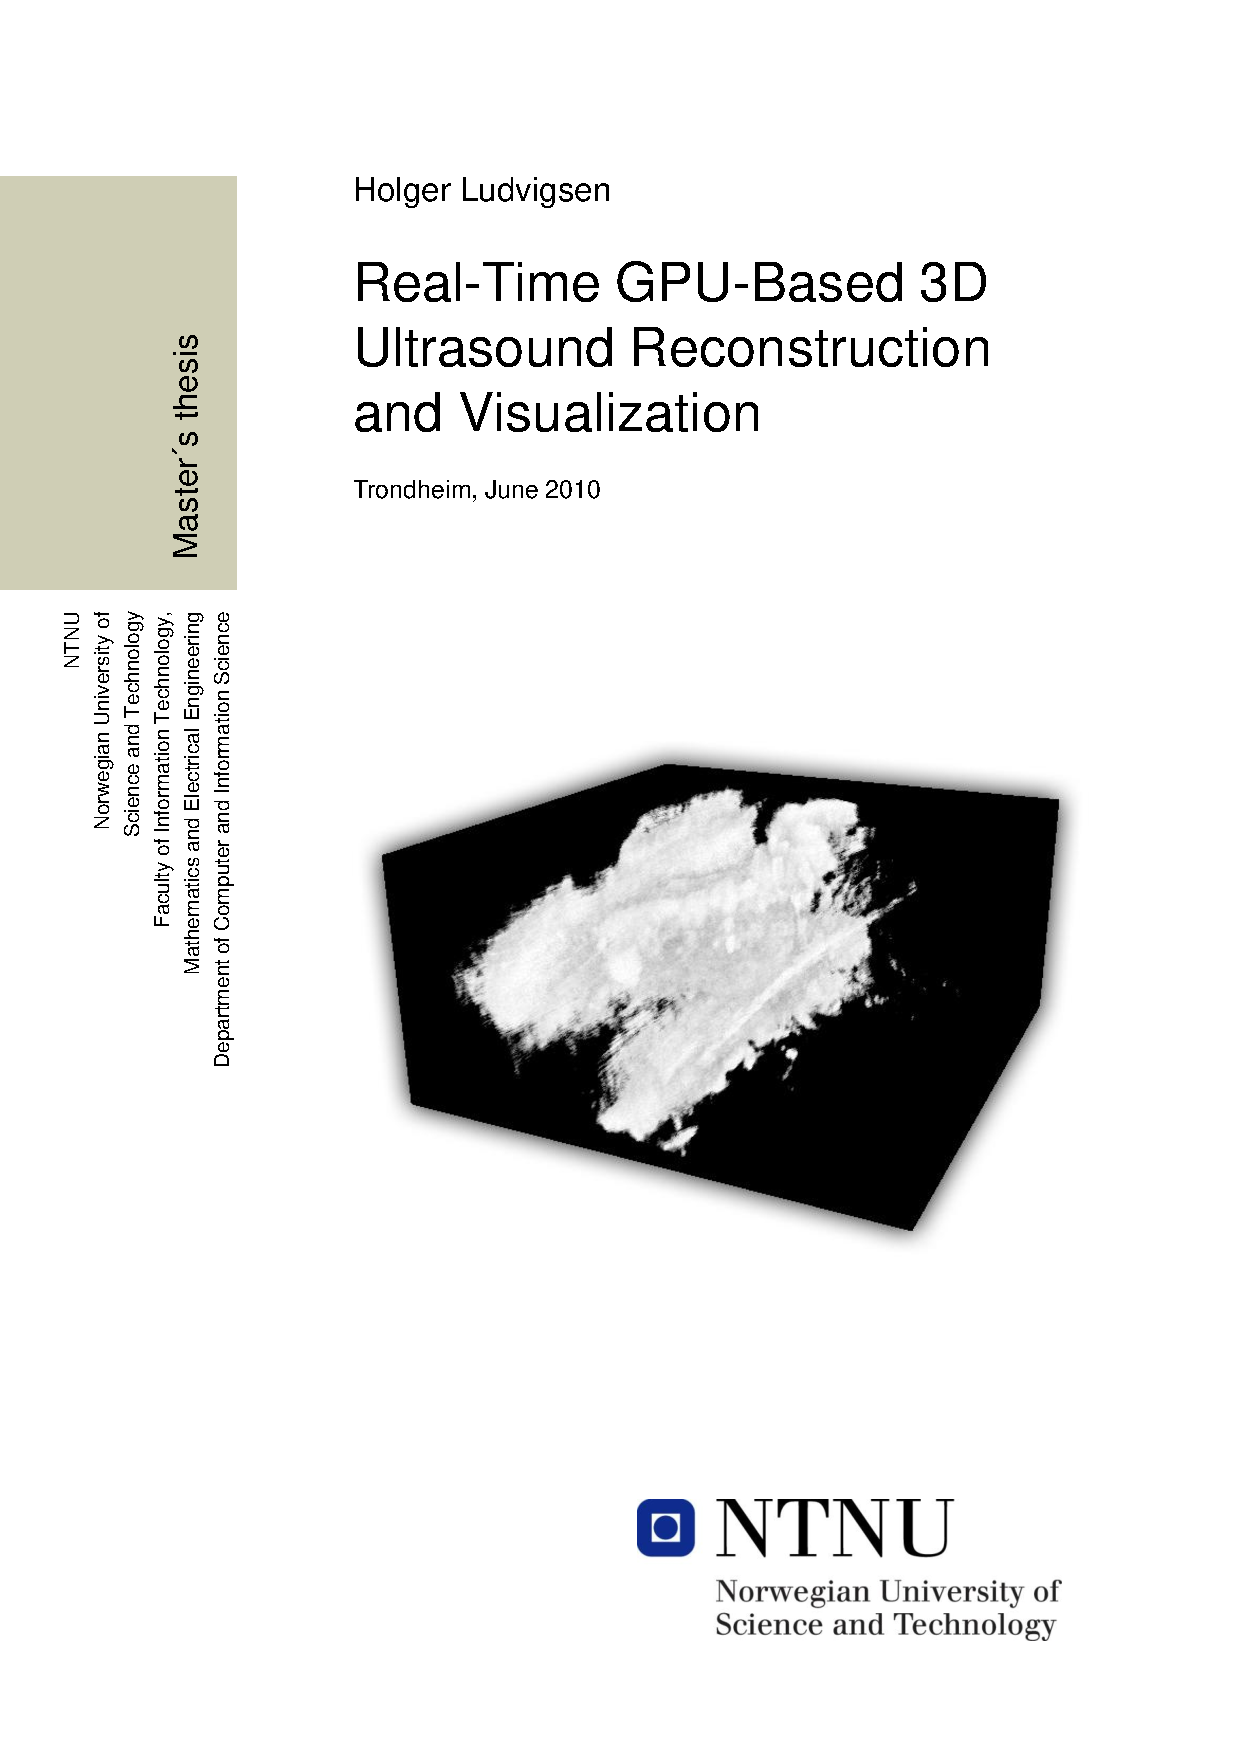
\includepdf[pages={1}]{graphics/cover.pdf}
%\cleardoublepage
%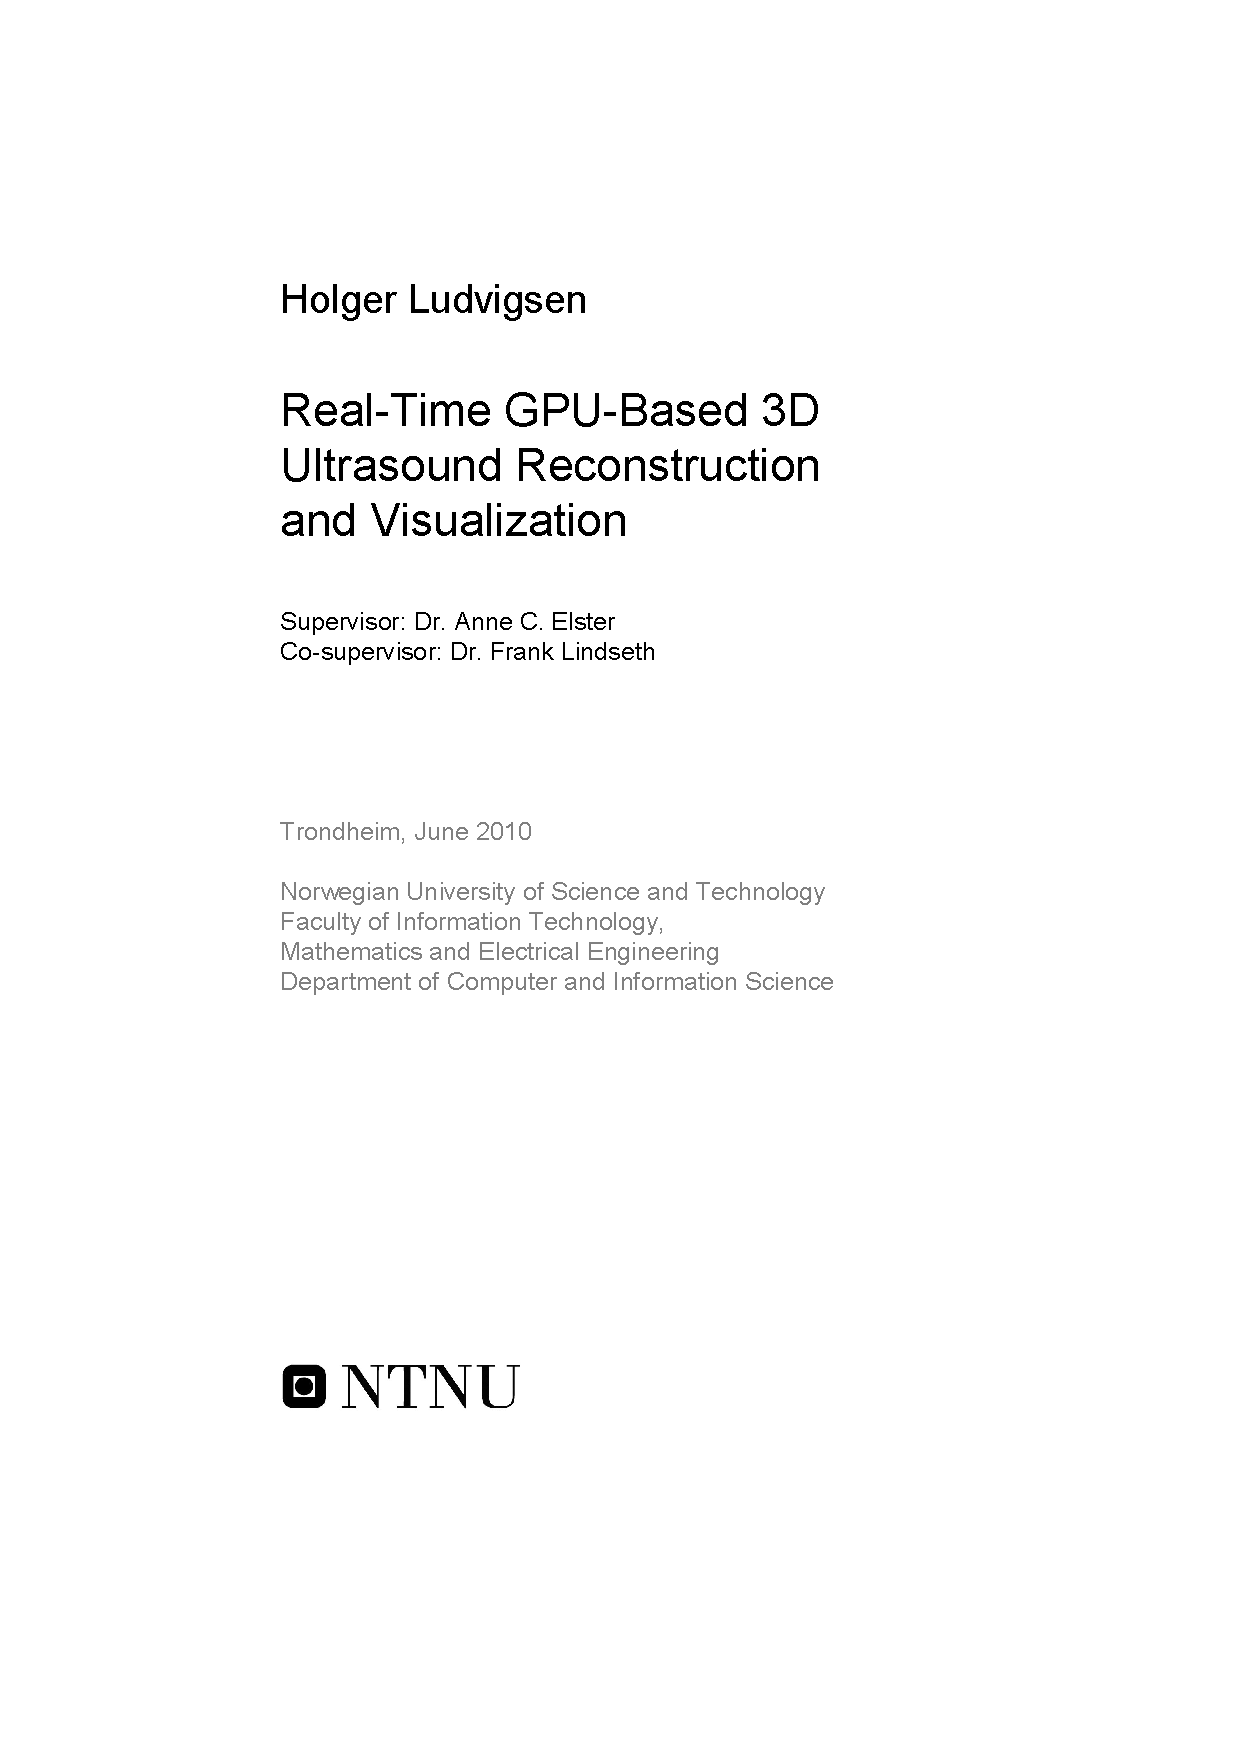
\includepdf[pages={1}]{graphics/titlepage.pdf}
%\cleardoublepage

%\chapter*{Problem Description}
%	\thispagestyle{empty}
%	3D ultrasound reconstruction can be used to generate volume data from tracked real-time 2D ultrasound frames. Compared to other imaging modalities like MRI and CT, ultrasound is a flexible low-cost solution for generating 3D image maps of the internal organs of the human body using existing 2D ultrasound scanners. This makes ultrasound the modality of choice for intraoperative use and enables image guided surgery (e.g.\ neuro- or laparoscopic) where surgical instruments are safely navigated inside the human body.

Current CPU-based methods for 3D ultrasound reconstruction are time consuming (typically from 1 minute to 1 hour depending on the quality). The overall goal of this thesis is to use GPU-based techniques to achieve real-time (or close to real-time) reconstruction and visualization of ultrasound.

\begin{description}
	\item[Step 1)] GPU-based real-time 3D ultrasound reconstruction of freehand 2D scans using a tracked ultrasound probe (different algorithms, command-line based).
	
	\item[Step 2)] Simultaneous reconstruction and visualization of the ultrasound volume as it gets built. It would be desirable for the surgeon to see a visualization of the volume while the data is acquired and the volume is generated (real-time volume rendering and slicing).
\end{description}

Technical issues such as parallelization and memory management techniques as well as recent platforms such as OpenCL, Nvidia Fermi and recent AMD graphics cards will also be evaluated.
%	\cleardoublepage
	
\chapter*{Abstract}
	\changepage{}{1.0cm}{-0.5cm}{-0.5cm}{}{}{}{}{} %\changepage{textheight}{textwidth}{evensidemargin}{oddsidemargin}{columnsep}{topmargin}{headheight}{headsep}{footskip}
	\addcontentsline{toc}{chapter}{Abstract}
	\pagenumbering{roman}
	\setcounter{page}{1}
	% what is the problem solved?
% how did we solve it?
% what were the results?
% what are the main findings/conclusions?

Ultrasound scanning is frequently used in medical practice because it is a non-invasive, safe and low-cost solution (\textit{vs.}\ CT or MR). However, conventional ultrasound probes only provide 2D scans. 3D ultrasound reconstruction builds 2D scans into 3D volumes of the patient's internals. Since these volumes can be used for acquiring out-of-angle views, 3D rendering of the anatomy, and for image guided surgery, they are rapidly expanding the possible uses of ultrasound. However, the 3D reconstruction process is computationally demanding and includes processing millions of picture and volume elements. This process can currently take minutes or even hours on conventional systems. 

It is very desirable to reconstruct ultrasound images in \emph{real-time} to guide surgeons doing surgery. In this thesis, we manage to achieve this by utilizing the parallel processing power of GPUs with hundreds of computing cores. Our novel optimized methods take advantage of this power in order to perform entire volume reconstructions in only \emph{fractions of a second}. Several optimization techniques have been developed, including only processing the relevant parts of the input. Novel methods for real-time incremental reconstruction producing high-quality results based on advanced interpolation techniques, are also presented. 

Using our novel pixel-based and voxel-based methods, we are able to generate a volume of 67 million voxels in on 0.9 and 0.6 seconds, respectively. These results are based on the new NVIDIA Fermi GPUs, OpenCL and 434 tracked ultrasound scans. For high-quality incremental reconstruction, real-time processing times are obtained for methods based on distance weighted orthogonal projections and on the probe trajectory (PT). Our GPU implementations give a performance speedup of 14 for pixel-based methods, an impressive 51 for voxel-based methods, and speedup of 6-8 for the incremental methods, compared with single-threaded CPU implementations. The cubic interpolation of the PT method is shown to be superior to the others and preserves the most details. As for possible future work, we point out techniques for handling memory constraints, complex probe movement and the device-to-host transfer bottleneck.
	\cleardoublepage
	\changepage{}{-1.0cm}{0.5cm}{0.5cm}{}{}{}{}{} %\changepage{textheight}{textwidth}{evensidemargin}{oddsidemargin}{columnsep}{topmargin}{headheight}{headsep}{footskip}

\chapter*{Acknowledgements}
	\addcontentsline{toc}{chapter}{Acknowledgements}
	This thesis is the result of work done at the HPC laboratory at the Department of Computer and Information Science (IDI) at the Norwegian University of Science and Technology (NTNU) in Trondheim, Norway. The work has been done in collaboration with the Department of Medical Technology at SINTEF in Trondheim, Norway.

I would like to thank my supervisor Dr. Anne C. Elster (IDI) and my co-supervisor Dr. Frank Lindseth (SINTEF, IDI) for their supervision and help in completing this thesis. Dr. Elster is the backbone and driver of the HPC group at IDI and NTNU, and this thesis would not have been possible without the resources she has made available for the students at the HPC laboratory. Dr. Lindseth is a world leader in medical ultrasound, and his knowledge and experience was invaluable during my work. I also want to thank Ole Vegard Solberg (SINTEF) for assistance and very helpful input. Some of the GPUs used in the work was donated to the laboratory by NVIDIA and AMD. I wish to thank NVIDIA and AMD for their support of the laboratory.

Finally, I would like to thank my fellow students at the HPC group for ideas and support, especially my good friend Ahmed A. Aqrawi for his camaraderie and humorous discussions during those countless hours at the lab.

\bigskip
\bigskip
\begin{center}
\emph{Trondheim, June 2010}
\end{center}
\begin{figure}[h]
\centering

\includegraphics[width=0.5\textwidth]{graphics/signature.png}
\caption*{Holger Ludvigsen}
\end{figure}
	\cleardoublepage

\addcontentsline{toc}{chapter}{Table of Contents}
\tableofcontents
\addcontentsline{toc}{chapter}{List of Figures}
\listoffigures
\addcontentsline{toc}{chapter}{List of Tables}
\listoftables

\chapter*{List of Abbreviations}
	\small
	\changepage{}{1.0cm}{-0.5cm}{-0.5cm}{}{}{}{}{} %\changepage{textheight}{textwidth}{evensidemargin}{oddsidemargin}{columnsep}{topmargin}{headheight}{headsep}{footskip}
	\addcontentsline{toc}{chapter}{List of Abbreviations}
	\begin{description}
	\item[B-scan] A 2D ultrasound image as acquired from an ultrasound machine
	\item[C2050] Nvidia Tesla C2050, a graphics card from Nvidia's GF100 (Fermi) architecture (released spring 2010) with 448 cores (see Table \ref{table:c2050hd5870} for specifications)
	\item[CPU] Central Processing Unit
	\item[CUDA] Compute Unified Device Architecture, a GPGPU architecture and API from Nvidia
	\item[Device] The device where parallel computations are offloaded to (e.g.\ GPU)
	\item[DWOP] Reconstruction method based on Distance Weighted Orthogonal Projections \cite{trobaugh1994}
	\item[FX5800] Nvidia Quadro FX5800, a graphics card from Nvidia's GT200 architecture preceding the GF100 with 240 cores (see Table \ref{table:c2050hd5870} for specifications)
	\item[GPGPU] General Purpose Computations on GPU
	\item[GPU] Graphical Processing Unit, an accelerator located on a graphics card and offloading graphical operations from the CPU
	\item[HD5870] AMD ATI Radeon HD5870, a graphics card from AMD's recent HD500 series with 320 cores (see Table \ref{table:c2050hd5870} for specifications)
	\item[Host] The system that contains \emph{devices} like GPUs
	\item[MPR] Multiplanar Reformatting, a technique for visualizing volumetric data by planar slices through the volume
	\item[NDRange] N-Dimensional Range, an index space for OpenCL work-items
	\item[PNN] Reconstruction method based on Pixel-Nearest-Neighbor \cite{mccann1988}
	\item[PT] Reconstruction method based on Probe Trajectory \cite{coupe2005}
	\item[ROI] Region-Of-Interest
	\item[VNN] Reconstruction method based on Voxel-Nearest-Neighbor \cite{sherebrin1996}
\end{description}
	\changepage{}{-1.0cm}{0.5cm}{0.5cm}{}{}{}{}{} %\changepage{textheight}{textwidth}{evensidemargin}{oddsidemargin}{columnsep}{topmargin}{headheight}{headsep}{footskip}
	\normalsize

\cleardoublepage

\pagestyle{fancy}
\fancyhead[R]{}

\chapter{Introduction}
	\pagenumbering{arabic}
	\setcounter{page}{1}
	
	% motivations
	% Repeat the motivation for the work
% Summarize what was done
% ? Explain why all goals have been met?

Ultrasound is a non-invasive, safe, low cost and practical way to provide medical doctors with an internal view of a patient's body. By performing 3D ultrasound reconstruction, 3D volumes can be constructed from 2D ultrasound scans, and be used for acquiring out-of-angle views, 3D rendering of the anatomy, and for image guided surgery. The purpose of this thesis was to investigate the parallel processing power of the GPU for fast ultrasound reconstruction. Having the ability to reconstruct a volume in a fraction of a second enables instant feedback and real-time incremental reconstruction while scanning. This thesis has presented our techniques to perform fast, non-incremental and real-time incremental reconstruction using the GPU. Optimization techniques for both pixel-based and voxel-based approaches have been described, and a novel method of doing real-time incremental reconstruction was presented. The performance obtained by these methods have been measured on some of the latest hardware architectures at the time of writing from both Nvidia and AMD. Issues for future work to look into are suggested in Section \ref{section:future_work}, and some final thoughts and closing statements are also given in Section \ref{section:final_thoughts}.
	
	\clearpage
	
	\section{Goals}
	
		% thesis goals
		%Step 1)
%GPU-based real-time 3D ultrasound reconstruction of freehand 2D scans using a tracked ultrasound probe (different algorithms, command-line based).

%Step 2)
%Simultaneous reconstruction and visualization of the ultrasound volume as it gets built. It would be desirable for the surgeon to see a visualization of the volume while the data is acquired and the volume is generated (real-time volume rendering and slicing).

The goals of this thesis are to:

\begin{itemize}
	\item Evaluate how to utilize the GPU in the most efficient manner to speed up computation time of 3D freehand ultrasound reconstruction.
	\item Develop methods to incrementally reconstruct the volume in real-time on the GPU as the data is acquired.
	\item While the data is being reconstructed on the GPU, visualize it in real-time.
\end{itemize}
		
	\section{Contributions}
	
		% thesis contributions
		The main contributions of this thesis are:

\begin{itemize}
	\item A novel method of doing real-time incremental 3D reconstruction using GPU and CPU.
	\item Optimization techniques for both pixel-based and voxel-based reconstruction on modern GPU architectures.
	\item A software implementation, called \emph{Thunder}, of GPU-based ultrasound reconstruction and visualization including:
	\begin{itemize}
		\item Fast reconstruction by voxel-based and pixel-based algorithms.
		\item High-quality reconstruction in real-time as data is acquired incrementally.
		\item Simultaneous reconstruction and visualization by both slices through the volume and ray casting on the GPU.
		\item Multiplatform implementation using the OpenCL standard with performance results on the newest GPU hardware architectures from Nvidia and AMD.
	\end{itemize}
\end{itemize}
	
	\section{Thesis Outline}
	
		The rest of the thesis is structured as follows:
	
\begin{description}
	\item[Chapter \ref{chapter:3d_ultrasonography}] introduces the field of 3D ultrasonography. Methods of reconstructing a volume from ultrasound scans and techniques to visualize the volume are described. Previous work in the field of ultrasound reconstruction and visualization is also presented.
	\item[Chapter \ref{chapter:gpgpu}] introduces general purpose computations on GPUs (GPGPU). A brief history and current state of GPU computing is presented, and the recent OpenCL architecture for GPGPU is described.
	\item[Chapter \ref{chapter:gpu_reconstruction}] describes the approach developed in this thesis where the GPU is utilized to perform fast reconstruction of ultrasound scans acquired in beforehand.
	\item[Chapter \ref{chapter:incremental_reconstruction_visualization}] describes the approach developed in this thesis for real-time incremental reconstruction and volume visualization performed on the GPU simultaneously as the data is acquired.
	\item[Chapter \ref{chapter:results_discussion}] presents the performance and quality of the ultrasound reconstruction and visualization as performed in this thesis. These results are also discussed together with other important issues.
	\item[Chapter \ref{chapter:conclusion_future_work}] summarizes the findings of the work described in this thesis and presents possible avenues of future work.
	\item[Appendix \ref{chapter:annotated_bib}] contains an annotated bibliography of selected references.
	\item[Appendix \ref{chapter:large_figures}] contains large uncropped versions of selected figures.
	\item[Appendix \ref{chapter:poster}] contains a poster summarizing the principles and main results of this thesis with focus on the incremental reconstruction.
	\item[Appendix \ref{chapter:test_measurements}] contains additional numerical test measurements.
	\item[Appendix \ref{chapter:optix_paper}] contains a paper about ray tracing on the GPU using the Nvidia OptiX library, including volume ray casting.
	\item[Appendix \ref{chapter:code_listings}] contains selected code listings from implementations of the methods described in this thesis.
	
\end{description}
	
\chapter{3D Ultrasonography}
	\label{chapter:3d_ultrasonography}
		
	% Repeat the motivation for the work
% Summarize what was done
% ? Explain why all goals have been met?

Ultrasound is a non-invasive, safe, low cost and practical way to provide medical doctors with an internal view of a patient's body. By performing 3D ultrasound reconstruction, 3D volumes can be constructed from 2D ultrasound scans, and be used for acquiring out-of-angle views, 3D rendering of the anatomy, and for image guided surgery. The purpose of this thesis was to investigate the parallel processing power of the GPU for fast ultrasound reconstruction. Having the ability to reconstruct a volume in a fraction of a second enables instant feedback and real-time incremental reconstruction while scanning. This thesis has presented our techniques to perform fast, non-incremental and real-time incremental reconstruction using the GPU. Optimization techniques for both pixel-based and voxel-based approaches have been described, and a novel method of doing real-time incremental reconstruction was presented. The performance obtained by these methods have been measured on some of the latest hardware architectures at the time of writing from both Nvidia and AMD. Issues for future work to look into are suggested in Section \ref{section:future_work}, and some final thoughts and closing statements are also given in Section \ref{section:final_thoughts}.
	
	\section{Medical Ultrasound}
	
		% about 3D ultrasound used in medicine
			\begin{figure}[t]
		\centering
		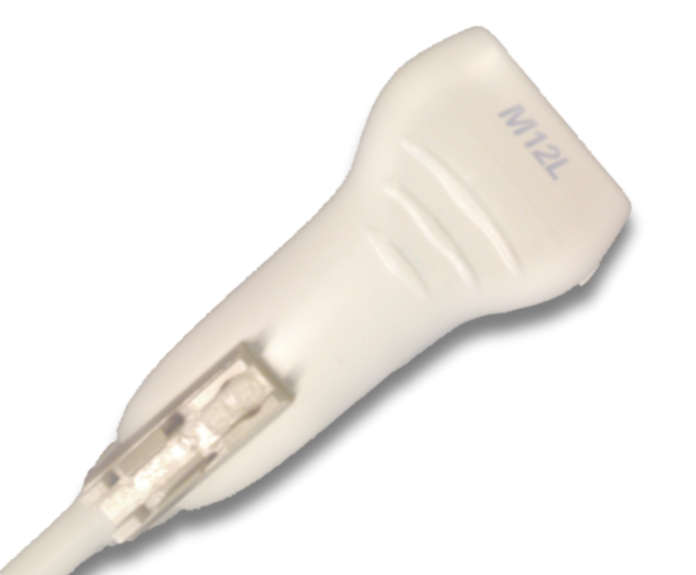
\includegraphics[height=0.3\textheight]{graphics/ultrasound_probe.png}
		\caption[Ultrasound probe]{GE M12L linear array ultrasound probe (GE Healthcare, Waukesha, Wisconsin, USA)}
		\label{fig:ultrasound_probe}
	\end{figure}

In medicine, ultrasound probes such as the one shown in Figure \ref{fig:ultrasound_probe} are used to obtain 2D ultrasound scans called \emph{b-scans}. The probe both emits ultrasound pulses and detects their echo returned. See Figure \ref{fig:ultrasound_principle} for an illustration. As the ultrasound pulse travels through tissue, echoes are created when it encounters materials with varying density. Some of the pulse energy is absorbed by the tissue, some is reflected back as echo and some continues to move forward.
	
	\begin{figure}[b]
		\centering
		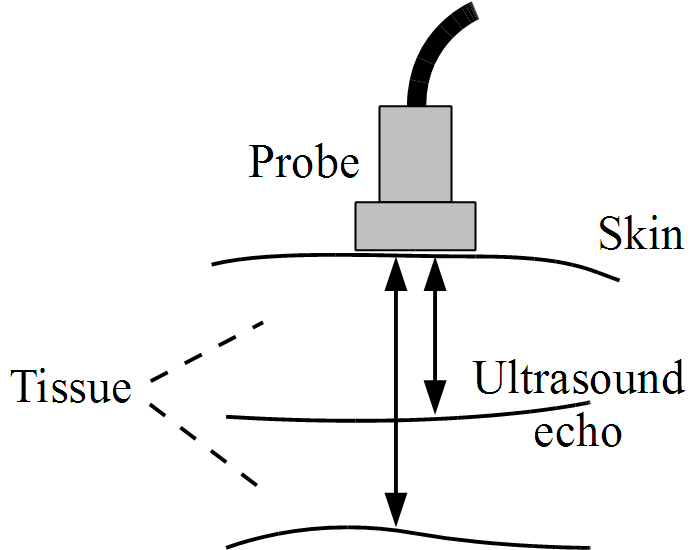
\includegraphics[height=0.25\textheight]{graphics/ultrasound_principle.png}
		\caption{The basic principles of ultrasound in medicine}
		\label{fig:ultrasound_principle}
	\end{figure}

The speed of sound depends on the transmission material, but one can assume a constant speed of $v_{sound} = 1540$ $m/s$ in human tissue \cite{anderson2000}. It should be noted that in reality the speed varies depending on the material, and can be as low as $1450$ $m/s$ in fat and over $1600$ $m/s$ in muscle, but we do not take this into consideration. This means that the distance $d$ from the transducer to the density variation can be estimated by the time $t$ it took for the echo to arrive at the transducer:

	\begin{equation}
		d = \frac{tv_{sound}}{2}
		\label{eq:ultrasound_distance}
	\end{equation}
	
The strength of the echo is given by the difference between acoustic impedances of the materials next to each other. If the probe emits and receives ultrasound in a linear array, a 2D image can be formed where the height is the distance from the probe, the width is the width of the array and the intensity of a pixel is the strength of the echo. The resulting image is the ultrasound b-scan. The array can also be curved, giving a \emph{curvilinear} b-scan. Examples of linear and curvilinear b-scans are shown in Figure \ref{fig:b-scan_examples}.

	\begin{figure}[h]
	\centering
	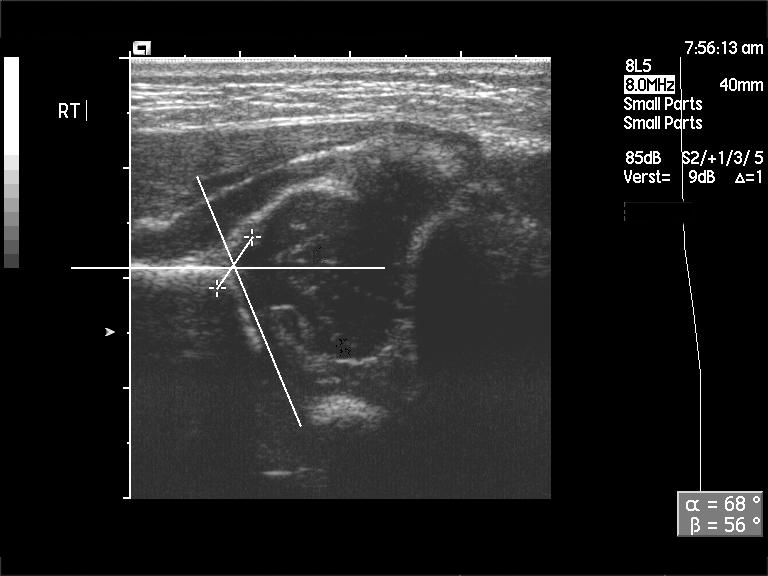
\includegraphics[width=0.49\textwidth]{graphics/linear_b-scan.png}
	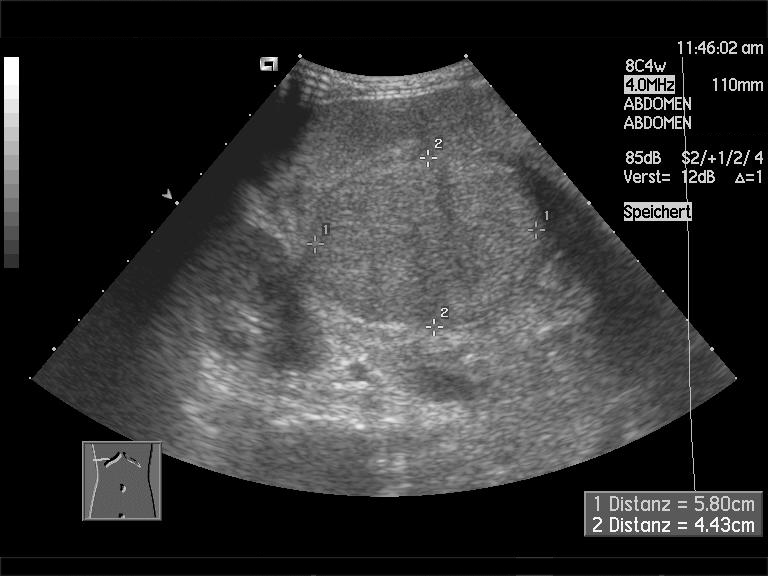
\includegraphics[width=0.49\textwidth]{graphics/curvilinear_b-scan.png}
	\caption[Linear and curvilinear b-scans]{Linear and curvilinear b-scans (used with permission from A. Christaras)}
	\label{fig:b-scan_examples}
	\end{figure}

To construct a 3D volume, each b-scan is tagged with a timestamp and location and rotation of the probe in 3D space. This data together with the b-scans is then processed, which can take minutes to hours depending on the desired quality of the reconstructed output. Once reconstructed, the volume can be used for many purposes. Typically, it can be visualized using direct volume rendering through ray casting or similar methods. But other techniques are also used, such as multiplanar reformatting slices (MPR slices) that are created from the volume. The MPR slices are planar slices of sampled points through the volume, like cutting it in half with a sharp flat knife. More details about visualization of 3D ultrasound data is found in Section \ref{section:ultrasound_visualization}, and description of how to reconstruct a volume from b-scans is found in Section \ref{section:ultrasound_reconstruction}.
		
	\section{Tracking in Ultrasound}
	
		Most reconstruction methods rely on an accurate tracking of the ultrasound probe, and there are several ways to obtain this. Most methods use either electromagnetic, optical, mechanical or acoustic sensors, but an alternative is to estimate the orientation from the ultrasound scans themselves. Such sensorless tracking can be done by analyzing speckle noise in the scans using decorrelation or linear regression techniques. However, sensorless systems do not offer the same accuracy as with actual sensors \cite{mercier2005}.

Mechanical tracking methods involve attaching the probe to structures with certain degrees of freedom, or letting a machine move the probe automatically. Disadvantages with this method is the reduced freedom and that additionally only one probe at the time can be tracked. Acoustic tracking uses sound emitters and receivers. The position can be tracked by measuring the time it takes for the sound to reach the receiver, or by measuring the relative phase shift when moving the probe. Disadvantages include the required line of sight for the sound waves, and varying speed of sound depending on factors such as temperature and pressure. Electromagnetic tracking systems measure current induced by moving a receiver in an electromagnetic field. This method has the advantage of being resistant against occlusion, but metallic objects as well as power sources or CRT monitors can distort the field.

An optical tracking system such as the one used for data collection for our thesis is shown in Figure \ref{fig:tracking_system}. Spheres that reflect infrared light are attached to the probe, and two cameras record the reflected infrared light. The position of the spheres relative to the cameras can then be used to estimate the location and orientation of the probe. Obviously, the system requires that the probe is in line of sight from the cameras.

	\begin{figure}[h]
	\centering
	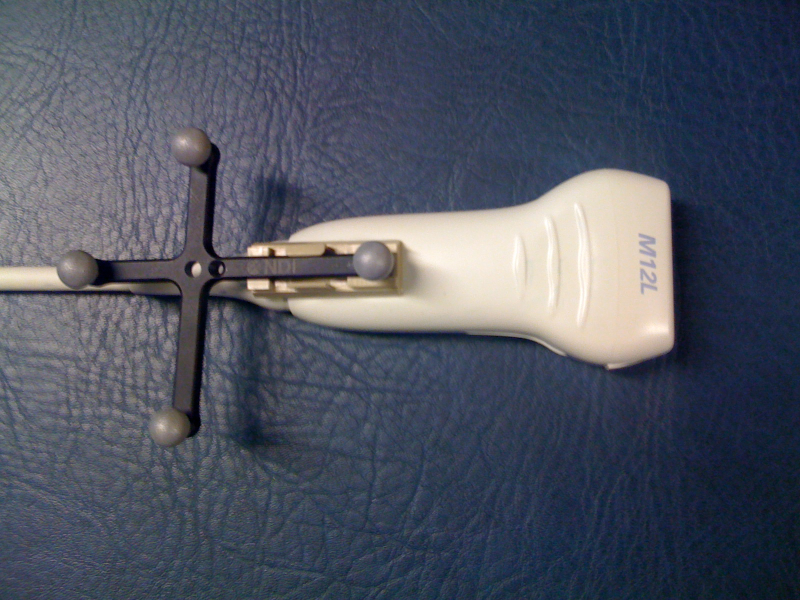
\includegraphics[height=0.23\textheight]{graphics/tracking_system_1.png}
	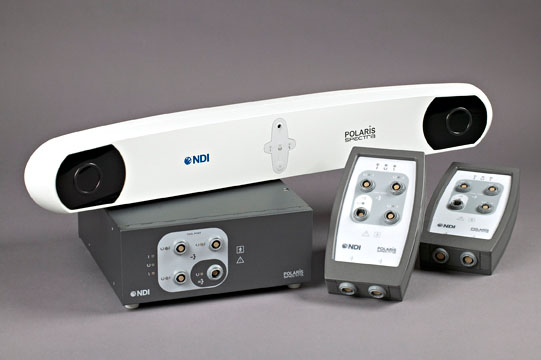
\includegraphics[height=0.23\textheight]{graphics/tracking_system_2.png}
	\caption[Linear array probe and optical tracking system]{GE M12L linear array probe (GE Healthcare, Waukesha, Wisconsin, USA) with tracking frame and Polaris Spectra optical tracking system (Northern Digital, Waterloo, Canada) (Photo of Polaris Spectra used with permission from Northern Digital Inc.)}
	\label{fig:tracking_system}
	\end{figure}
	
	\section{3D Ultrasound Reconstruction}
		\label{section:ultrasound_reconstruction}
	
		% intro/motivation, rough explanation of forward and backward approaches, then outline of section
There is more than one approach to reconstructing a 3D volume from a series of 2D b-scans. Two main categories of algorithms exist: \emph{pixel-based} and \emph{voxel-based} reconstruction. These are sometimes also called \emph{forward} and \emph{backward} reconstruction, and this section describes the two approaches.
%A technique for accelerating voxel-based methods, called fast slice selection, is also described.
The section also describes the basics of geometric transformations in 3D space that are used by these methods.

% about transformation matrices
\subsection{Geometric Transformations}

	A geometric transformation is an operation on a set of coordinates \cite{eberly2004}. Operations that can be applied include rotation, translation, resizing and skewing. A practical way to represent a transformation on a set of initial coordinates $\bb{P}$, is by a \emph{transformation matrix} $\bb{T}$:
	
	\begin{equation}
		\bb{S} = \bb{T} \cdot \bb{P}
		\label{eq:transformation}
	\end{equation}
	
	where $\bb{S}$ are the transformed coordinates. To make it possible to represent translation by transformation matrices, we convert $\bb{P}$ to \emph{homogenized coordinates} $\bb{P}'$ by extending it with one dimension with a scalar value of 1. Given that $\bb{P}$ is a vector of $N$ dimensions, then $\bb{P}'$ is of $N+1$ dimensions and $\bb{T}$ is a $(N+1) \times (N+1)$ matrix. The product $\bb{T} \cdot \bb{P}'$ will then give a homogenized $N+1$ vector that can be converted to normal coordinates by dividing each element by the value of the added dimension. Typically as this value is still 1, we can simply omit the last dimension.
	
	The identity matrix represent an empty transformation with no effect. The transformations used in this thesis are rotations and translations. Equation \ref{eq:transformation_matrices_0} give a translation matrix and Equations \ref{eq:transformation_matrices_1}, \ref{eq:transformation_matrices_2} and \ref{eq:transformation_matrices_3} give rotation matrices around the x, y and z axis, 
	
	\begin{equation}
		\bb{T}_{translate} =
		\left[ {\begin{array}{cccc}
		1 & 0 & 0 & x \\
		0 & 1 & 0 & y \\
		0 & 0 & 1 & z \\
		0 & 0 & 0 & 1 \\
		\end{array} } \right]
		\label{eq:transformation_matrices_0}
	\end{equation}
	
	\begin{equation}
		{\bb{T}_{rotate}}_x =
		\left[ {\begin{array}{cccc}
		1 & 0 & 0 & 0 \\
		0 & \cos{\theta} & -\sin{\theta} & 0 \\
		0 & \sin{\theta} & \cos{\theta} & 0 \\
		0 & 0 & 0 & 1 \\
		\end{array} } \right]
		\label{eq:transformation_matrices_1}
	\end{equation}
	
	\begin{equation}
		{\bb{T}_{rotate}}_y =
		\left[ {\begin{array}{cccc}
		\cos{\theta} & 0 & \sin{\theta} & 0 \\
		0 & 1 & 0 & 0 \\
		-\sin{\theta} & 0 & \cos{\theta} & 0 \\
		0 & 0 & 0 & 1 \\
		\end{array} } \right]
		\label{eq:transformation_matrices_2}
	\end{equation}
	
	\begin{equation}
		{\bb{T}_{rotate}}_z =
		\left[ {\begin{array}{cccc}
		\cos{\theta} & -\sin{\theta} & 0 & 0 \\
		\sin{\theta} & \cos{\theta} & 0 & 0 \\
		0 & 0 & 1 & 0 \\
		0 & 0 & 0 & 1 \\
		\end{array} } \right]
		\label{eq:transformation_matrices_3}
	\end{equation}
	
	where $(x, y, z)$ are the translations in the x, y and z dimension and $\theta$ is the rotation angle. Representing combined translation and rotation is simply done by multiplying transformation matrices into one matrix. An example involving a translation and two rotations is given below:
	
	\begin{equation}
		\bb{S} = \bb{T}_{translate} \cdot {\bb{T}_{rotate}}_x \cdot {\bb{T}_{rotate}}_y \cdot \bb{P} = \bb{T}_{combined} \cdot \bb{P}
		\label{eq:transformation_combination_1}
	\end{equation}
	
	where
	
	\begin{equation}
		\bb{T}_{combined} = \bb{T}_{translate} \cdot {\bb{T}_{rotate}}_x \cdot {\bb{T}_{rotate}}_y
		\label{eq:transformation_combination_2}
	\end{equation}
	
	The orientation of an ultrasound b-scan can be represented by a transformation matrix that is given by a tracking system (which is the case in this thesis).

% what is the pixel based approach to reconstruction?
\subsection{Pixel-Based Reconstruction}

	Pixel-based reconstruction, also known as forward reconstruction, iterates over the ultrasound b-scans and attempts to project their values into a volume. The term pixel-based comes from that this approach involves processing each b-scan pixel, and since the b-scans are the input, and the volume is the output this is dubbed as a forward method, as opposed to the voxel-based method described in the next section.
	
	For each b-scan $j$ with orientation given by $\bb{T}_j$, each pixel $i$ on the b-scan at location $(x_i, y_i, 0)$ with intensity $c_{j,i}$ has a contribution $V_{i,j}$ to the volume given by:
	
	\begin{equation}
		V_{i,j}(x, y, z) = m(x_i, y_i) w(|(x, y, z) - \bb{T}_j \cdot (x_i, y_i, 0)|) c_{j,i}
	\end{equation}
	
	where $w$ is a weighting function and $m$ is a 2D mask function defining a region-of-interest (ROI) in the b-scan with the value 1 inside the region and 0 outside. The weighting function can be based on the distance between the voxel and the pixel, and examples of such weighting functions include Gaussian bell (Equation \ref{eq:gaussian}) and inverse distance (Equation \ref{eq:inverse}) \cite{gonzalez2008}.
	
	\begin{equation}
		w_{Gaussian}(x) = ae^{-{\frac{(x-b)^2}{2c^2}}}
		\label{eq:gaussian}
	\end{equation}
	
	\begin{equation}
		w_{inverse}(x) = \frac{1}{x}
		\label{eq:inverse}
	\end{equation}
	
	To perform pixel based reconstruction, the following algorithm can be used as basis (based on \cite{solberg2007}):
	
	\begin{itemize}
		\item for each b-scan $j$:
		\begin{itemize}
			\item for each pixel $i$ inside mask:
			\begin{itemize}
				\item $v =$ the coordinates of the pixel in volume space.
				\item for each voxel $v'$ in kernel $k$ around $v$:
				\begin{itemize}
					\item add to the voxel's value the pixel's value weighted by the weighting function $w$.
				\end{itemize}
			\end{itemize}
		\end{itemize}
	\end{itemize}
	
	A number of variations of this basic algorithm exist. The size of the kernel and the definition of the weighting function can obviously be changed, and the simplest case is to let the pixel contribute to only the closest voxel without any weighting. This is called pixel-nearest-neighbor (PNN).
	
	A problem with PNN is that some voxels may never be filled from any pixels, and this is especially a problem when adjacent b-scans are far apart and thus have much space between them. To fix this, a hole-filling stage is required after the PNN volume filling. This can be done by iterating over all unfilled voxels and set them to the average of all filled neighbors in a kernel around them.
	
	A consideration needs to be done when filling a voxel with a value, as it might already be filled from another pixel. The scheme chosen is called a \emph{compounding method}. Common compounding methods are:
	
	\begin{itemize} 
		\item overwrite the old value
		\item overwrite the old value only if the voxel has not yet been filled
		\item compute an average/median of the values
		\item keep the maximum value
	\end{itemize}
	
	If overwriting, one can lose data if the new value is erroneous due to noise in tracking data or ultrasound sensoring. Averaging reduces noise, but smudges the volume. Keeping the maximum can be useful to avoid deleting values by overwriting them with empty (i.e. dark, low-intensity) values.

% what is the voxel based approach to reconstruction?
\subsection{Voxel-Based Reconstruction}

	Voxel-based reconstruction methods iterates over the volume to be reconstructed and for each voxel determines which pixels influence it. This is called a backwards method since it is based on the output (the volume). Some of the principles explained for pixel-based methods also apply in voxel-based methods: Pixels outside the mask should not influence the volume and a compounding method must be chosen.
	
	Each voxel is processed to determine which pixels influence it, and how they do it. Several variants of voxel-based reconstruction exist, but the following algorithm can be used as a basis (based on \cite{solberg2007}):
	
	\begin{itemize}
		\item for each voxel $j$:
		\begin{itemize}
			\item for each b-scan $i$ that is close to the voxel $j$:
			\begin{itemize}
				\item for each pixel $p$ in $i$ that is inside the mask:
				\begin{itemize}
					\item add to the voxel's value the pixel's value weighted by the weighting function $w$.
				\end{itemize}
			\end{itemize}
		\end{itemize}
	\end{itemize}
	
	Several variants of voxel-based methods exist. If only the closest pixel to the voxel is used without any weighting, then the method is called voxel-nearest-neighbor (VNN). Since all voxels are traversed in voxel-based reconstruction, no hole-filling is necessary.
	
% what is the probe trajectory method?
%\subsection{Reconstruction Based on Probe Trajectory}

	% Perhaps explain this in the implementation chapter?
		
	\section{3D Ultrasound Visualization}
		\label{section:ultrasound_visualization}
	
		%intro
One of the purposes of doing incremental reconstruction is to be able to see the volume as it is constructed. This allows for immediate feedback during scanning. There are many ways to visualize a volume, and the system described in this thesis offers orthogonal multiplanar reformatting (MPR) slices or volume ray casting. In addition, as the volume is accessible on both device and host memory, it can be used as input for third-party visualization packages. In this section, the visualization techniques used are described.

\subsection{Orthogonal MPR slices}
% pictchaz
% volume on CPU, slices extracted (no interpolation because of orthogonal along axis)
% how used OpenGL
% explain user interface (mouse rotate and index incr/decr)

\begin{figure}[h]
\centering
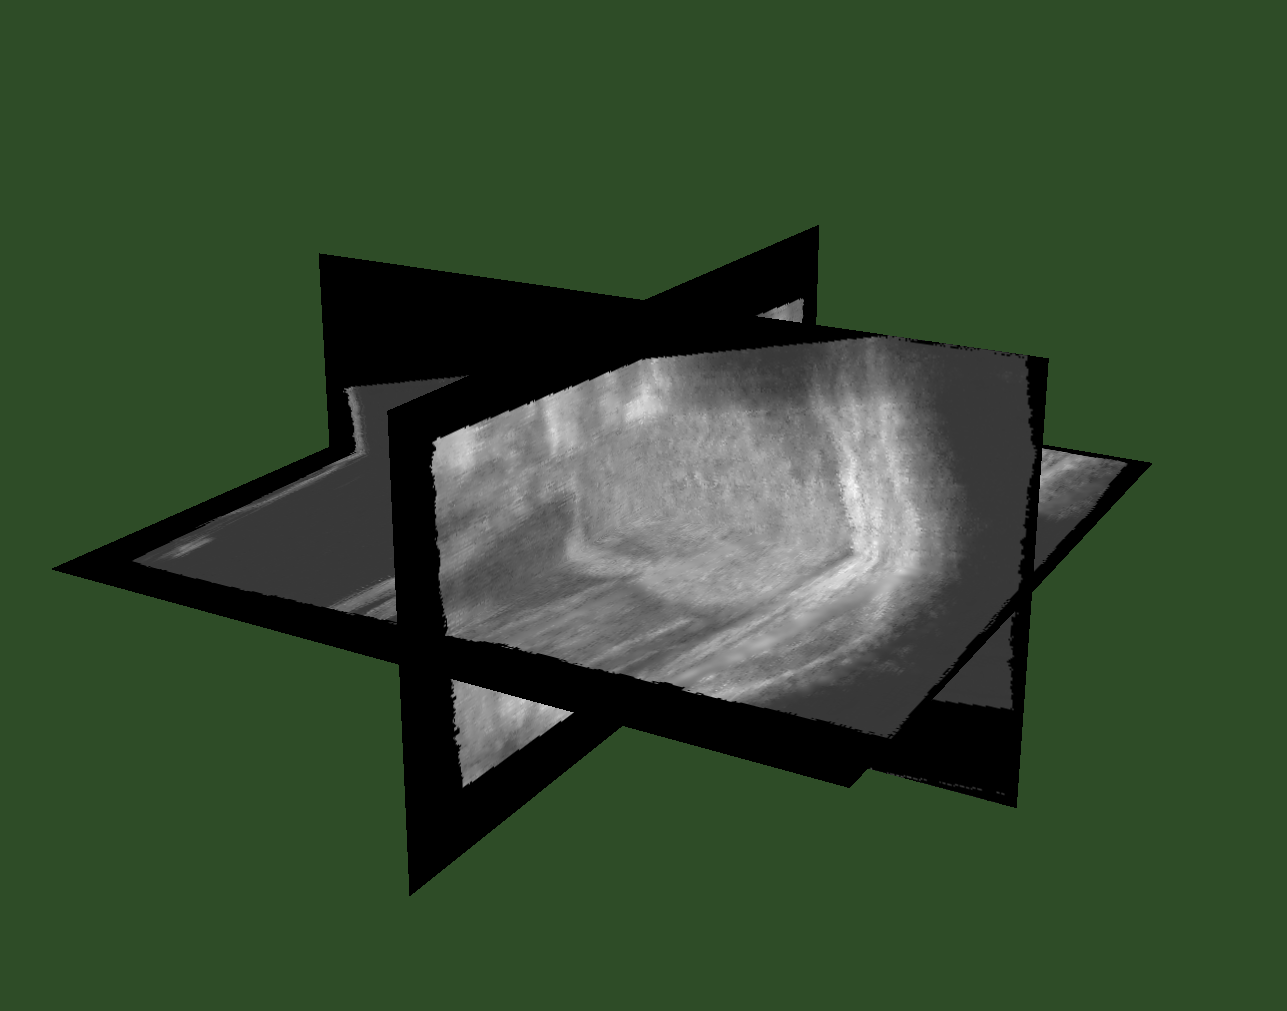
\includegraphics[width=0.49\textwidth]{graphics/orthogonal_screen0.png}
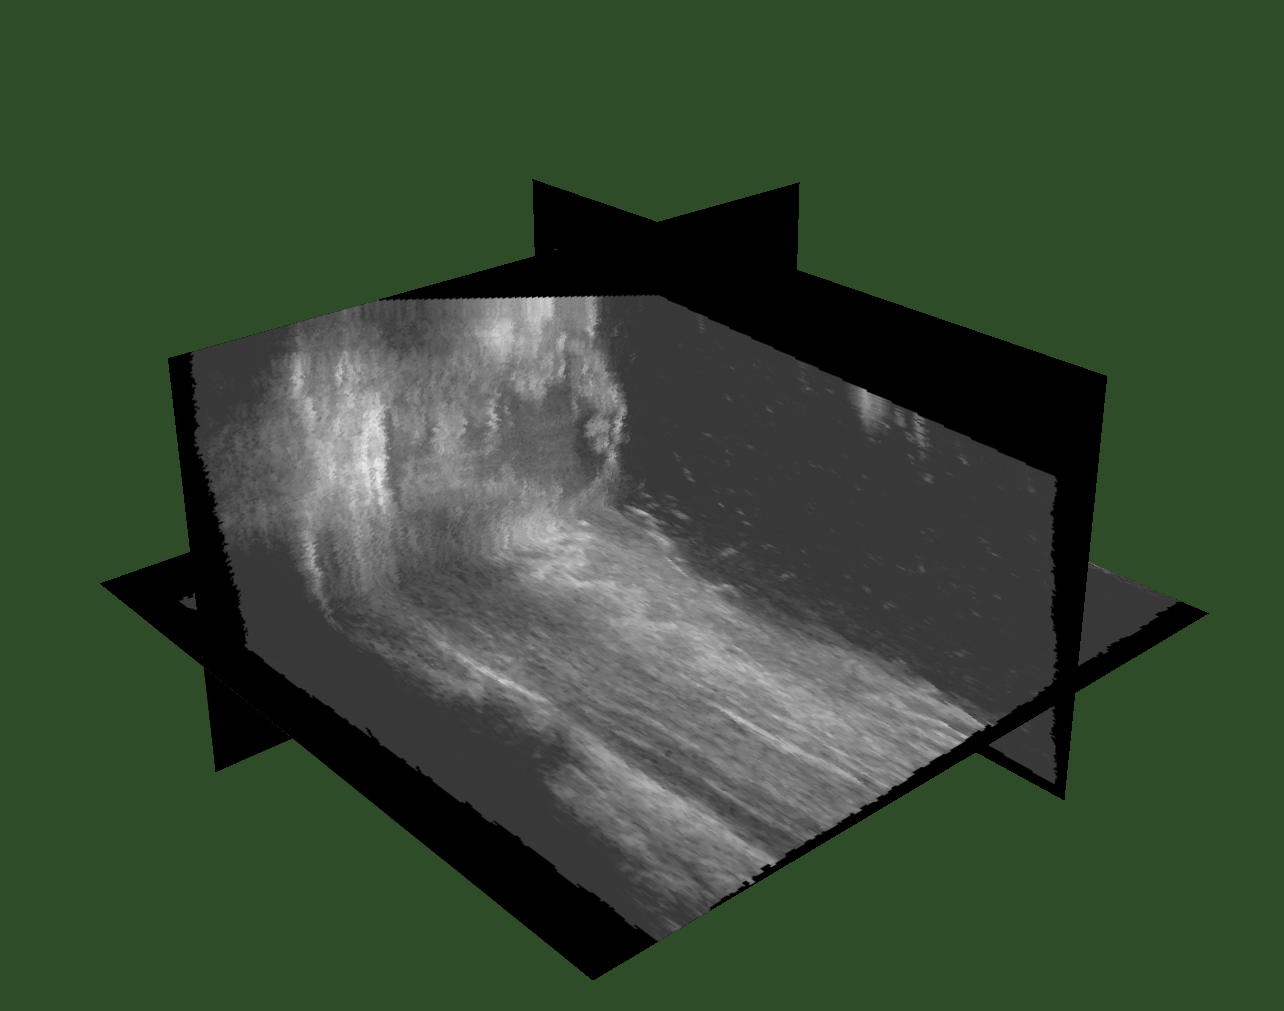
\includegraphics[width=0.49\textwidth]{graphics/orthogonal_screen1.png}
\caption[Screenshots of orthogonal MPR slices]{Screenshots of orthogonal MPR slices generated by our implementation}
\label{fig:orthogonal_screens}
\end{figure}

Figure \ref{fig:orthogonal_screens} shows some screenshots of the orthogonal MPR slices, and larger figures can be found in Appendix \ref{chapter:large_figures}. The slices are along each of the three volume axis, and the voxel values in each slice are rendered on the slice plane. This is performed by extracting voxel values on indices $(x,y,i)$, $(x,i,z)$ and $(i,y,z)$ for the z, y and x axis, respectively. The parameter $i$ determines where on each axis the slices are located, while $x$, $y$ and $z$ are all the possible voxel indices in the volume. The slices are extracted from the host memory volume and used as textures for three orthogonal polygons rendered with OpenGL. It should be noted that extracting the voxels and using them as textures takes a negligible amount of time. Using the mouse, the user can rotate the volume to view the slices at different angles, and pressing keyboard keys will increase or decrease the $i$ parameter. In this way, all parts of the volume can be visualized.

\subsection{Volume Ray Casting}
% pictchaz
% volume ray casted while on GPU
% one thread per ray
% build ray dirs kernel
% cast rays kernel
% do box-ray intersection to skip to volume before stepping
% set strength to max_voxel
% for each step:
	% if strength below cutoff -> end stepping
	% calculate transparency: min(1-voxel/max_voxel + adjustment, 1)
	% (if voxel below (other) cutoff -> set transparent to 1 (due to grey US background))
	% accumulate strength*(1-transparency)
	% update strength by multiplying with transparency
% set pixel to ray accumulation

\begin{figure}[h]
\centering
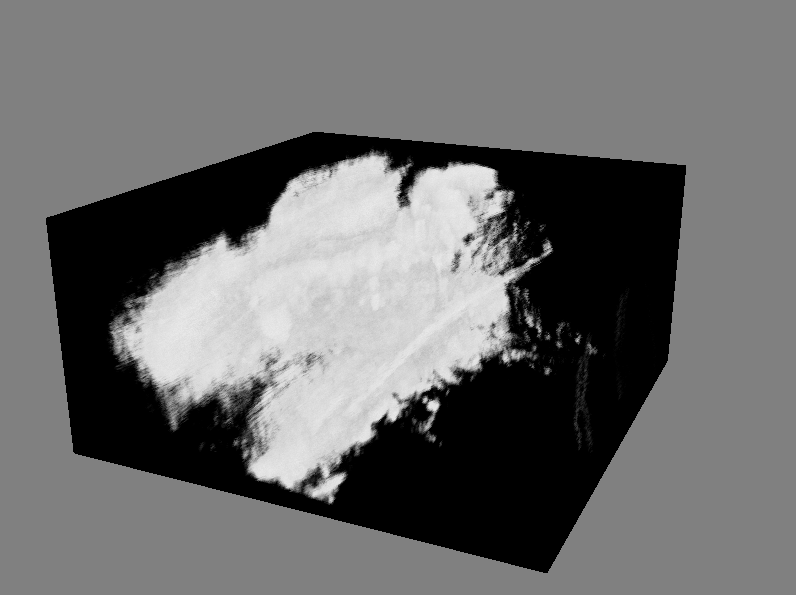
\includegraphics[width=0.49\textwidth]{graphics/raycast_screen0.png}
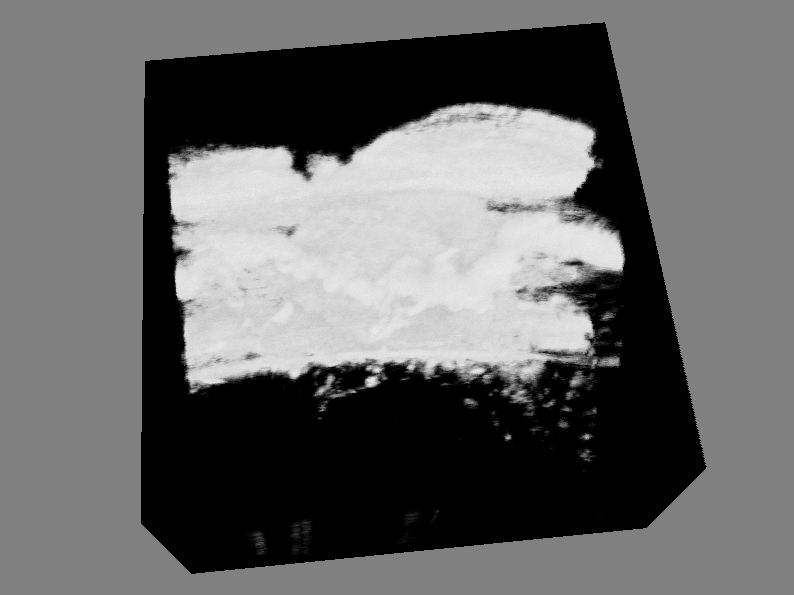
\includegraphics[width=0.49\textwidth]{graphics/raycast_screen1.png}
\caption[Screenshots of volume ray casting]{Screenshots of volume ray casting generated by our implementation}
\label{fig:raycast_screens}
\end{figure}

Figure \ref{fig:raycast_screens} shows some screenshots of the ray casted volume, and larger figures can be found in Appendix \ref{chapter:large_figures}. Ray casting is a computationally demanding task, but the GPU's processing power is utilized while the volume data is still on the device memory. The task is parallelized with one thread per ray, and consists of two steps: first construct the rays, then cast them into the volume.

Code listings of the implemented OpenCL kernels can be found in Appendix \ref{section:ray_casting_kernel}. The resulting rendered image consists of $w_s \times h_s$ pixels, with one ray (and thread) per pixel. The camera is defined by a camera location in space, a \emph{lookat} location that the camera is looking at, a vector defining "up" in the rendered image, and a vector defining "flat" (the horizontal direction) in the rendered image. Each ray's origin is the given camera location, but their direction needs to be calculated from their pixel position and a desired field-of-view. %This is done with Equation \ref{eq:ray_dir}.

%\begin{equation}
%	\label{eq:ray_dir}
%	r = \left| |camera_{lookat}-camera_{pos}| + FOV_{hor} camera_{right} \frac{x_{ray} - \frac{w_s}{2}}{\frac{w_s}{2}} + FOV_{vert} camera_{up} \frac{y_{ray} - \frac{h_s}{2}}{\frac{h_s}{2}} \right|
%\end{equation}

When the ray directions have been found, they can be cast into the volume. Instead of stepping from the ray origin, we save computations by first calculating the intersection between the box-shaped volume and each ray. This saves sampling for steps that are outside the volume.

There are many ways to accumulate voxel intensities while stepping along a ray. The method used in this work models the voxels as transparent cubes with a transparency level between 0.0 (fully oblique) and 1.0 (invisible). The entire procedure is as follows:

\begin{enumerate}
	\item $strength = 255$
	\item for each step along ray:
	\begin{enumerate}
		\item if $strength <$ cutoff, then break stepping
		\item $transparency = 1-\frac{intensity_{voxel}}{255}$
		\item accumulate $strength \cdot (1-transparency)$ into ray's pixel intensity
		\item $strength \leftarrow strength \cdot transparency$
	\end{enumerate}
\end{enumerate}

Each ray starts with a \emph{strength} parameter representing how much light has been absorbed. The initial value is the maximum value of a pixel (255), and it is reduced for each voxel encountered. For each voxel sampled, its intensity is weighted by the current strength and accumulated into the final pixel intensity. To save computations, the stepping is ended if the strength is below a given cutoff where the voxels simply do not contribute noticeable intensities.
		
	\section{Previous Work on 3D Ultrasound Reconstruction}

		% presentation of important previous work in the field including that which this thesis directly builds upon in the form of a consequtive text with cites
		Previous work in the field of 3D ultrasound reconstruction include novel reconstruction algorithms and methods, as well as designed and implemented production systems. The field of ultrasound and volume visualization is extensive in itself. Nelson \textit{et al.}\ \cite{nelson1993} present approaches to visualization of 3D ultrasound data including simple ray casting and MPR slice visualization, and Ludvigsen \textit{et al.}\ \cite{ludvigsen2010} describe GPU-based volume ray casting with the Nvidia OptiX library. The rest of this section will focus on work in 3D ultrasound reconstruction. In Appendix \ref{chapter:annotated_bib}, an annotated bibliography of selected references can be found.

\subsection{Categorization of Reconstruction Methods}

The vast number of existing reconstruction approaches have been reviewed and categorized. Fenster \textit{et al.}\ \cite{fenster1996} present several approaches in 3D ultrasound imaging not limited to how to just reconstruct, but also the acquisition of input data and how to render the reconstructed results. An attempt at grouping existing reconstruction algorithms is done by Rohling \textit{et al.}\ \cite{rohling1999}. Their categorization of the methods is broadly defined as either \textit{voxel nearest-neighbor interpolation}, \textit{pixel nearest-neighbor interpolation} or \textit{distance-weighted interpolation}. Solberg \textit{et al.}\ \cite{solberg2007} present a different grouping that take additional types of algorithms into account and has a clearer separation between categories. Their grouping is into \textit{voxel-based}, \textit{pixel-based} and \textit{function-based} methods, and their work also includes a thorough comparison of the algorithms based on performance and quality.

\subsection{Implemented Reconstruction Systems}

Trobaugh \textit{et al.}\ \cite{trobaugh1994} present a formative description of a system where optical tracking is used to orient a freehand ultrasound probe, and includes volume reconstruction by both a voxel-based and a pixel-based method. A different approach is described by Prager \textit{et al.}\ \cite{prager1998}. Their \textit{Stradx} system does not reconstruct a volume, but instead generates MPR slices directly from the ultrasound b-scans. Welch \textit{et al.}\ \cite{welch2000} describes a volume reconstructing system under development that allows for updates to the volume during scanning and also simultaneous visualization at \emph{near} real-time performance. Another attempt presented by Gobbi \textit{et al.}\ \cite{gobbi2002} consists of an implemented system that does simultaneous real-time 3D ultrasound reconstruction and visualization, but is limited to the simple PNN method and only orthogonal MPR slice visualization. Furthermore, the visualization is not synchronous with the reconstruction, and is updated at a lower non-real-time framerate.

\subsection{Reconstruction Algorithms}

3D ultrasound reconstruction is often a trade-off between performance and quality. Trobaugh \textit{et al.}\ \cite{trobaugh1994} and Gobbi \textit{et al.}\ \cite{gobbi2002} use the simple PNN method to enable high performance. The alternative voxel-nearest-neighbor is used by Sherebrin \textit{et al.}\ \cite{sherebrin1996} in their 3D ultrasound system. Barry \textit{et al.}\ \cite{barry1997} use a more sophisticated pixel-based method with an inverse distance weighting kernel around inserted pixels. Different approaches are described by Rohling \textit{et al.}\ \cite{rohling1999} and Sanches \textit{et al.}\ \cite{sanches2000} that fall into the function-based category according the terminology of Solberg \textit{et al.}\ \cite{solberg2007}. Rohling \textit{et al.}\ use splines to construct a volume from the input b-scans, and Sanches \textit{et al.}\ use statistical methods to estimate a function for the interpolation. A recent voxel-based method is described by Coupe \textit{et al.}\ \cite{coupe2005} that takes the probe trajectory into account to improve reconstruction quality, especially for sparse input where there is much space between the b-scans. A performance increasing scheme for fast slice selection is described by Wein \textit{et al.}\ \cite{wein2006} and benefits voxel-based reconstruction methods. Karamalis \textit{et al.}\ \cite{karamalis2009} describe a high performing hybrid reconstruction method partially implemented using GPU texture interpolation features. Huang \textit{et al.}\ \cite{huang2005} describe a technique for utilizing the Fourier domain to take redundant frequency components into account, preserving the high frequencies and resulting in better resolutions.
		
\chapter{General Purpose Computations on GPUs}
	\label{chapter:gpgpu}

	% Repeat the motivation for the work
% Summarize what was done
% ? Explain why all goals have been met?

Ultrasound is a non-invasive, safe, low cost and practical way to provide medical doctors with an internal view of a patient's body. By performing 3D ultrasound reconstruction, 3D volumes can be constructed from 2D ultrasound scans, and be used for acquiring out-of-angle views, 3D rendering of the anatomy, and for image guided surgery. The purpose of this thesis was to investigate the parallel processing power of the GPU for fast ultrasound reconstruction. Having the ability to reconstruct a volume in a fraction of a second enables instant feedback and real-time incremental reconstruction while scanning. This thesis has presented our techniques to perform fast, non-incremental and real-time incremental reconstruction using the GPU. Optimization techniques for both pixel-based and voxel-based approaches have been described, and a novel method of doing real-time incremental reconstruction was presented. The performance obtained by these methods have been measured on some of the latest hardware architectures at the time of writing from both Nvidia and AMD. Issues for future work to look into are suggested in Section \ref{section:future_work}, and some final thoughts and closing statements are also given in Section \ref{section:final_thoughts}.
	
	\section{GPGPU Computing}
	
		% about GPGPUs history and current state
		GPU technology was developed for graphics processing in computer games for the purpose of offloading calculations involved in 2D and 3D graphics from the CPU. Early GPUs were fixed hardware accelerators specialized to perform the most common graphical operations. Graphical applications have the tendency to involve the same computations on different data, thus the GPU employs massive hardware parallelism for the computations. As an example, consider the task of rotating an object in 2D graphical applications \cite{hearn2004}. Each point $\bb{P}_i$ is rotated into $\bb{S}_i$:

	\begin{equation}
		\bb{S}_i = \bb{R} \cdot \bb{P}_i
		\label{eq:rotation_transform}
	\end{equation}
	
	where \bb{R} is a $2 \times 2$ rotation matrix and the same for all points. Each rotated point $\bb{S}_i$ can be evaluated individually in parallel. With e.g.\ thousands of points, this can reduce computation time drastically compared to evaluating them one by one after each other. Fixed function GPUs have since evolved into programmable units with the same parallel architecture, but where the parallel operations can be programmed for each stage of the graphics pipeline. Although meant for graphics processing such as 3D shading, these programmable GPUs have started to be used for general purpose computations. Applications that have a natural affinity for the GPU architecture involve executing similar calculations on thousands, if not millions, of data elements. GPU manufacturers such as Nvidia and AMD have recognized this potential in their products, and have released GPGPU frameworks such as Nvidia's CUDA (Compute Unified Device Architecture) \cite{kirk2010, cudaprogguide} and AMD's ATI Stream technology \cite{streamreleasenotes}.
	
\subsubsection{Current state of GPGPU}

	 Many examples of utilizing the GPU for general purpose computations exist. In the field of medical ultrasound, Nielsen \cite{nielsen2007} uses the GPU for image enhancement of ultrasound through the wavelet transform. Another example is Herikstad \cite{herikstad2009}, who estimates and corrects aberration in ultrasound scans on the GPU.

	The third generation of Nvidia GPUs targeting GPGPU computing are based on the GF100 architecture. The GF100 is used in Nvidia products such as the GeForce GTX470 for computer games and Tesla C2050 for high performance computing. AMD's competing GPU generation is the HD5000 series, which is used in products such as HD5870. Specifications for the C2050 and HD5870 series are given in Table \ref{table:c2050hd5870}. The Nvidia Quadro FX5800, which is similar to the Nvidia Tesla C1060 from Nvidia's second GPU generation is included for comparison and since it is also used for test measurements in this thesis. Note that memory bandwidth and performance are highly theoretical figures stated by the manufactorers \cite{c2050, fx5800, hd5870}.
	
	\begin{table}[h]
	\centering
	\begin{tabular}{| l l l l |}
		\hline
		\textbf{GPU} & \textbf{C2050 \cite{c2050}} & \textbf{FX5800 \cite{fx5800}} & \textbf{HD5870 \cite{hd5870}} \\
		\textbf{\# of cores} & 448 & 240 & 320\footnotemark[1] \\
		\textbf{Clock frequency} & 1150 MHz & 1296 MHz & 850 MHz \\
		\textbf{Memory} & 3 GB & 4 GB & 1 GB  \\
		\textbf{Theoretical} & & & \\
		\textbf{memory bandwidth} & 144 GB/s & 102 GB/s & 153 GB/s \\
		\textbf{Theoretical} & & & \\
		\textbf{performance} & 1030 GFLOP/s & 933 GFLOP/s & 2720 GFLOP/s \\
		\hline
	\end{tabular}
	\caption[Nvidia C2050, FX5800 and AMD HD5870 specifications]{Nvidia C2050, FX5800 and AMD HD5870 specifications}
	\label{table:c2050hd5870} % this table is referred to in section Test Setup in results-discussion chapter and in list of abbreviations
	\end{table}
	
	\footnotetext[1]{HD5870 has 320 \emph{stream cores} with a total of 1600 \emph{processing elements}}

	\section{OpenCL}
	
		% about OpenCL
		Open Computing Language Specification (OpenCL) is an open royalty-free standard for general purpose parallel programming \cite{openclspec} designed to be independent of platform and vendor, whether it be CPU, GPU or other class of accelerator. A detailed investigation of OpenCL and comparison with CUDA can be found in \cite{fagerlund2008}. The OpenCL standard consists of an architecture, an API and a programming language. The architecture is a model of the environment that the computations are performed in, including computational devices such as GPUs and a host system such as a x86 platform that contains the devices. The API is an interface for the host system to build, launch and coordinate parallel computations on the devices. The programming language is a version of the C programming language intended for writing the programs, termed \emph{kernels}, that are executed in parallel on the devices.

A readily available implementation of OpenCL is provided by Nvidia based on their CUDA architecture \cite{cudaprogguide}. There are over one hundred million GPUs sold that can execute CUDA programs. Additionally, AMD also has support for OpenCL as part of their ATI Stream technology \cite{streamreleasenotes}. So there is lots of hardware out there to exploit.

\subsection{OpenCL Architecture}

	The OpenCL architecture defines models for the host system and its computation devices, how the parallel computations are enqueued and executed, and the memory hierarchy on the devices.

	\subsubsection{Platform Model}
	
		Figure \ref{fig:opencl_platform} depicts the OpenCL platform model. The \emph{host} system is connected to one or more \emph{devices}. The devices consist of one or more \emph{compute units} that have a number of \emph{processing elements}. These processing elements do the actual computations. An example of a host system is a x86 desktop computer. Typical devices include GPUs, digital signal processors (DSPs), IBM and Sony's CELL BE processors and even multicore CPUs.
	
		\begin{figure}[h]
		\centering
		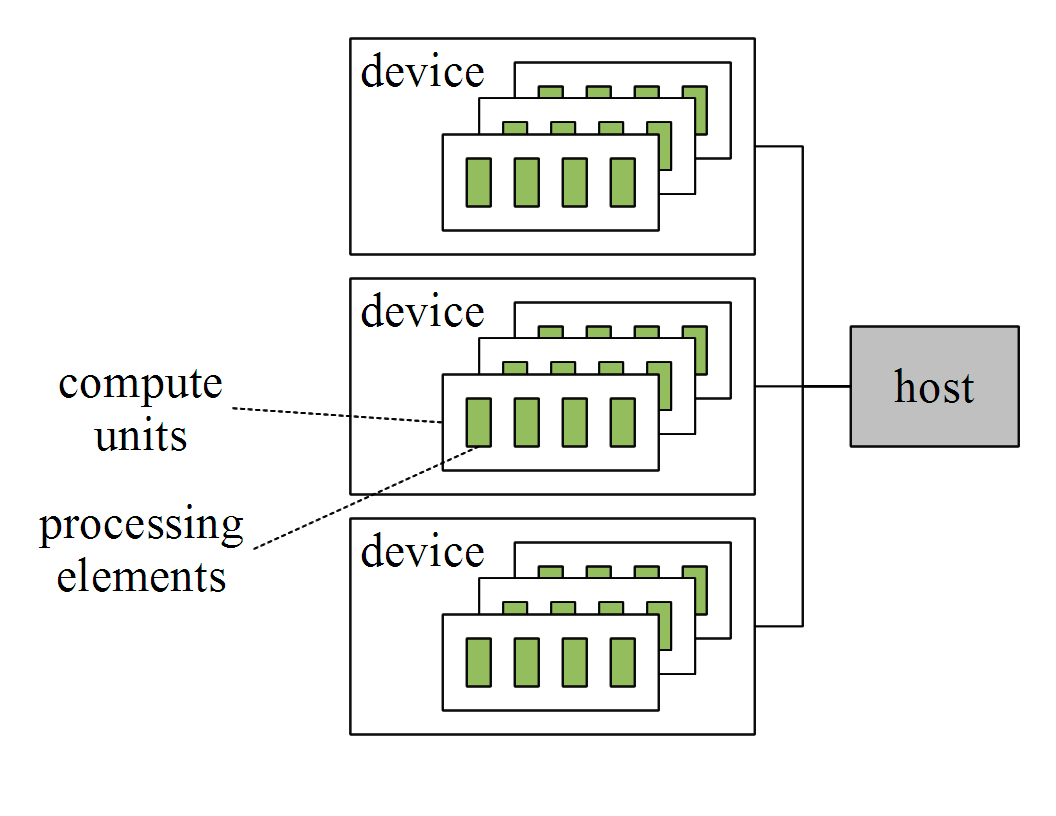
\includegraphics[height=0.35\textheight]{graphics/platform_model.png}
		\caption{OpenCL platform model}
		\label{fig:opencl_platform}
		\end{figure}
	
	\subsubsection{Execution Model}
		
		Figure \ref{fig:opencl_execution} shows the OpenCL execution model. The model is based on the single-instruction multiple-data model where the same operations are performed on different pieces of data. In OpenCL terminology, a \emph{work-item} is a thread that executes a \emph{kernel}. The kernel is written in the OpenCL C-based programming language, which will be described later. Work-items are organized in one, two or three dimensional \emph{work-groups}, and all the work-groups make up a \emph{NDRange} which is an index space in the same number of dimensions as the work-groups. Each work-item has a unique index in this \textit{NDRange}.
		
		\begin{figure}[h]
		\centering
		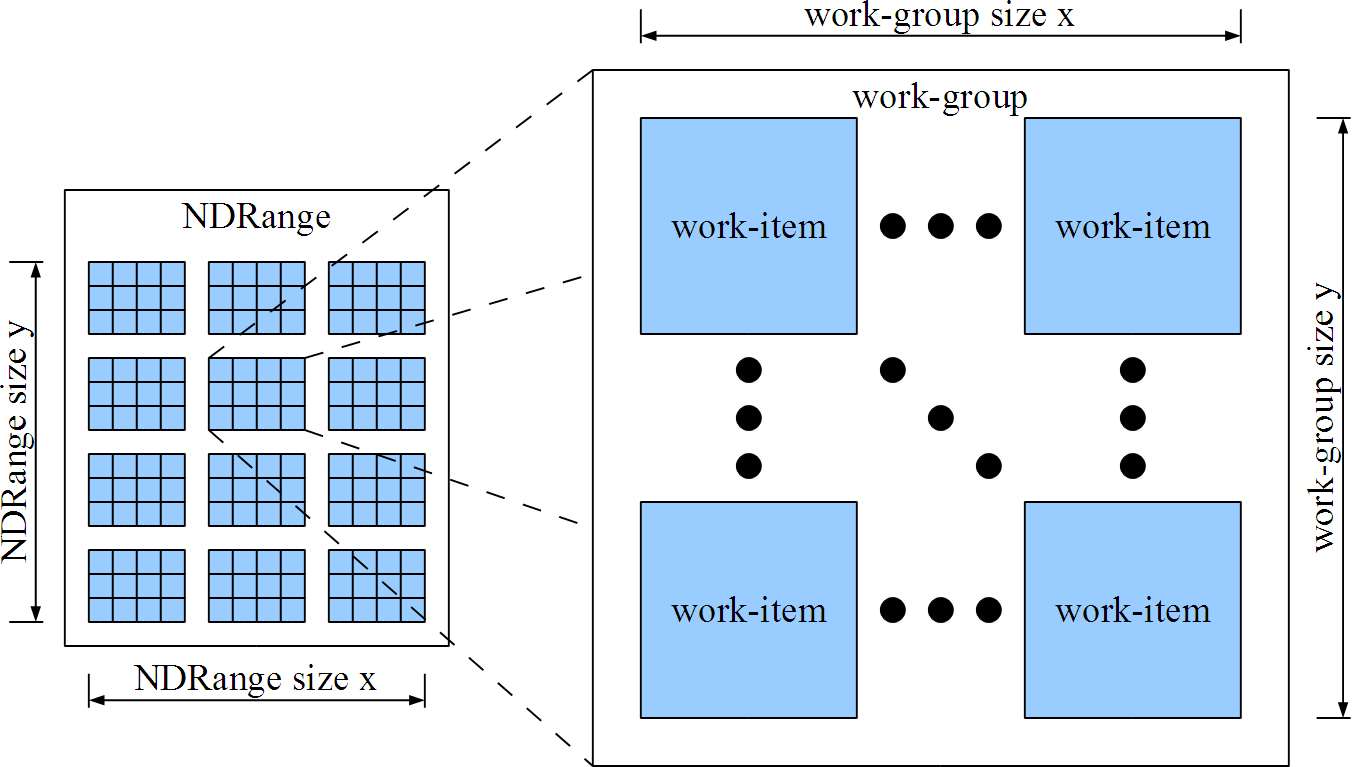
\includegraphics[width=1\textwidth]{graphics/execution_model.png}
		\caption{OpenCL execution model}
		\label{fig:opencl_execution}
		\end{figure}
		
		The execution of parallel kernels, memory transfers and synchronization in OpenCL is organized through \emph{command queues}. The tasks are called \emph{commands}, and are inserted into queues to be performed on or in association with a device. The order of execution can be either synchronous (\emph{in-order}) or asynchronous (\emph{out-of-order}). When in-order, the commands are launched and completed in the order they appear in the queue. When out-of-order, the commands are launched in order, but are not guaranteed to complete in order. The execution environment is defined by a \emph{context} which holds all the objects used during execution, such as devices, memory and command queues. Figure \ref{fig:command_queues} shows a context containing command queues that are mapped to devices.
		
		\begin{figure}[h]
		\centering
		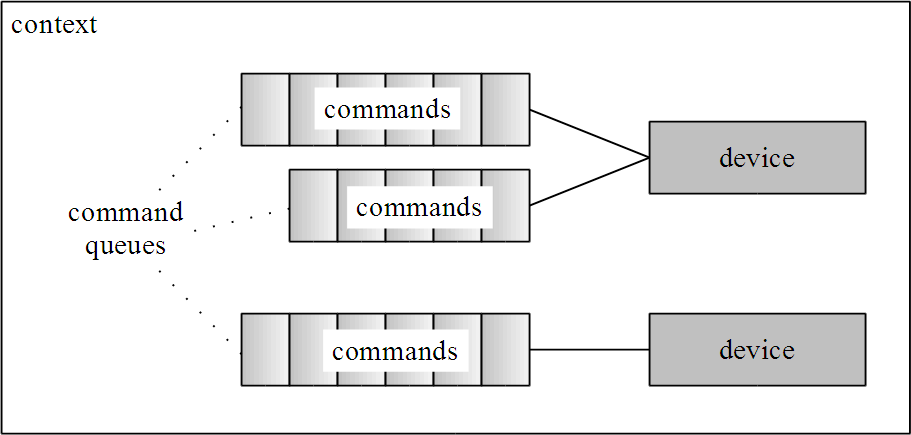
\includegraphics[height=0.25\textheight]{graphics/command_queues.png}
		\caption{OpenCL command queues and devices}
		\label{fig:command_queues}
		\end{figure}
	
	\subsubsection{Memory Model}
	
		Figure \ref{fig:opencl_memory} shows the OpenCL memory model. The model is closely tied to the platform model. The main memory on the device is the \emph{global memory}, which together with the read-only \emph{constant memory} is read- and writeable by the host system. Global and constant memory may be cached on the device. Each compute unit has a \emph{local memory} with the scope of individual work-groups, and each processing element has a \emph{private memory} where data with local scope to individual work-items is stored. Private and local memory are not directly accessible from host.
	
		\begin{figure}[h]
		\centering
		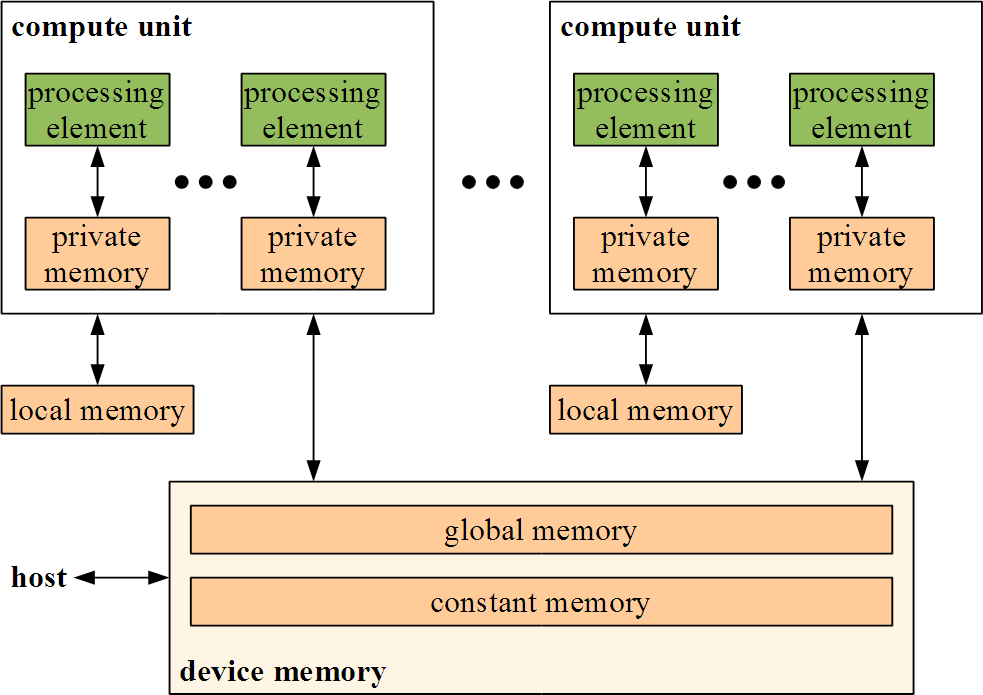
\includegraphics[width=0.9\textwidth]{graphics/memory_model.png}
		\caption{OpenCL memory model}
		\label{fig:opencl_memory}
		\end{figure}
		
\subsection{OpenCL \textit{vs.}\ CUDA}

	Historically, Nvidia's CUDA precedes OpenCL. CUDA was initially launched as a host API and programming model for Nvidia's GPUs. It's popularity made it a \emph{de facto} standard for GPGPU development. Nvidia has taken this a step further and introduced a GPU architecture dubbed the CUDA architecture, and Nvidia's OpenCL implementation runs on the CUDA architecture. Even though CUDA is an architecture, the CUDA API and programming model still exists and is heavily used, and the OpenCL architecture clearly resembles the CUDA architecture. Thus, at the time of writing, OpenCL is an alternative to the CUDA API and programming model. However, Nvidia has implemented the OpenCL standard on top of their CUDA architecture, and in a similar fashion AMD has implemented OpenCL on their ATI Stream technology.
	
	Some major concepts in OpenCL are analogue to concepts in CUDA. For readers experienced with CUDA, Table \ref{table:opencl_vs_cuda} shows CUDA terminology and corresponding equivalent in OpenCL.
	
	\begin{table}[h]
	\centering
	\small
	\begin{tabular}{| l l |}
		\hline
		\textbf{OpenCL terminology} & \textbf{CUDA terminology} \\
		\hline
		\hline
		kernel & kernel \\
		host & host \\
		NDRange & grid \\
		work-item & thread \\
		work-group & block \\
		global memory & global memory \\
		constant memory & constant memory \\
		local memory & shared memory \\
		private memory & local memory \\
		compute unit & stream multiprocessor \\
		processing element & core \\
		image & texture \\
		\hline
	\end{tabular}
	\caption{OpenCL \textit{vs.}\ CUDA terminology}
	\label{table:opencl_vs_cuda}
	\end{table}

\subsection{Host Programming in OpenCL}

	OpenCL provides a host API for building, launching and coordinating parallel computations on devices. It is also possible to extract platform dependent parameters such as memory sizes, maximum work-item sizes and other platform capabilities. This section explains how to use memory, program and kernel objects from the host system, and how to perform synchronization of the parallel computations. For a complete overview, see \cite{openclspec}.

	\subsubsection{Using Memory Objects}
	
		A \emph{memory object} is a part of device memory together with its attributes. By creating memory objects, the host allocates memory on the device. There are two types of memory objects. \emph{Buffers} are sequential arrays of scalar data types such as integers or floating point numbers, and are accessed as a series of bytes. \emph{Images} are two- or three- dimensional arrays for the purpose of containing images such as textures. An important difference between images and buffers is that images are accessed through \emph{samplers} with defined mechanisms for out-of-range coordinates, interpolation between values and filtering. This section will focus on buffer objects.
		
		Creating a buffer object is performed by the \texttt{clCreateBuffer} function:
		
		\begin{verbatim}
		cl_mem clCreateBuffer(cl_context context,
		                      cl_mem_flags flags,
		                      size_t size,
		                      void * host_ptr,
		                      cl_int * errorcode_ret)
		\end{verbatim}
		
		where \texttt{context} is the OpenCL context that will contain the buffer; \texttt{flags} are one or more flags defining attributes of the buffer as given in Table \ref{table:buffer_flags}; \texttt{size} is the buffer size in bytes and \texttt{host\_ptr} is an optional host memory pointer that is used depending on the flags given. The function returns a device memory pointer to the allocated buffer. \texttt{clCreateBuffer} also returns an error code in \texttt{errorcode\_ret} that is not equal to 0 if something went wrong, as most of the other OpenCL API calls also do.
		
		\begin{table}[h]
		\centering
		\begin{tabular}{| p{0.3\textwidth} p{0.65\textwidth} |}
			\hline
			\multicolumn{1}{|c}{\textbf{Flag}} & \multicolumn{1}{c|}{\textbf{Description}} \\
			\hline
			\hline
			\texttt{CL\_MEM\_READ\_WRITE} & Default flag. Buffer is read and written by kernels \\
			\texttt{CL\_MEM\_WRITE\_ONLY} & Write-only access from kernels \\
			\texttt{CL\_MEM\_READ\_ONLY} & Read-only access from kernels \\
			\texttt{CL\_MEM\_USE\_HOST\_PTR} & Use previously allocated \texttt{host\_ptr} as the storage area for the buffer instead of device memory \\
			\texttt{CL\_MEM\_ALLOC\_HOST\_PTR} & Allocate \emph{new} memory on host instead of device \\
			\texttt{CL\_MEM\_COPY\_HOST\_PTR} & Copy data from given \texttt{host\_ptr} to new buffer \\
			\hline
		\end{tabular}
		\caption{OpenCL buffer flags}
		\label{table:buffer_flags}
		\end{table}
		
		\clearpage
		
		Reading and writing buffer objects is performed by the \texttt{clEnqueue[Read|Write]Buffer} functions:
		
		\begin{verbatim}
		cl_int clEnqueue[Read|Write]Buffer(cl_command_queue cmd_queue,
		                                   cl_mem buffer,
		                                   cl_bool blocking,
		                                   size_t offset,
		                                   size_t size,
		                                   void * ptr,
		                                   cl_uint num_events,
		                                   cl_event * event_list,
		                                   cl_event * event)
		\end{verbatim}
		
		where \texttt{cmd\_queue} is the command queue that enqueues the read/write operation, \texttt{buffer} is the buffer object of \texttt{size} bytes and \texttt{blocking} is true/false depending on if the function should be blocking or not. If blocking is enabled, the function will not return until reading/writing has completed. \texttt{offset} is an offset into the buffer object to write or read from and \texttt{ptr} is a pointer to the location on the host to be written to or read from by the procedure.
		
		All functions that enqueue commands optionally have an associated \emph{event object} returned via the parameter \texttt{event}, that can be used to query for the status of the command or wait for its completion (if non-blocking). Furthermore, \texttt{event\_list} can contain a list of \texttt{num\_events} events that needs to be completed before this command is executed.
		
	\subsubsection{Using Program and Kernel Objects}
	
		An OpenCL \emph{program} is a set of kernels that can be built (compiled and linked) and be executed on specified devices. The kernel is usually defined by a string of code in the OpenCL C-based programming language, but can also be a previously compiled binary. The approach described here takes kernels as code strings. The program is created with the \texttt{clCreateProgramWithSource} function and built with the \texttt{clBuildProgram} function, respectively. For clarity, their argument lists are not stated explicitly here, but can be found in \cite{openclspec}.
		
		When the program is built, it is possible to create, set arguments to, and execute \emph{kernel objects} with the functions \texttt{clCreateKernel}, \texttt{clSetKernelArg} and \texttt{clEnqueueNDRangeKernel}. To create a kernel, a successfully built program and a kernel name is supplied. The total size of the arguments cannot exceed a platform dependent maximum (e.g.\ 4352 bytes for Quadro FX5800). Kernels are enqueued on a command queue like the buffer read/write operations. When enqueueing a kernel, the size and dimensionality of the \textit{NDRange} that it will operate on must be specified. A \emph{global work size} is given in $n$ work dimensions and defines the total number of work-items in the \textit{NDRange}. An $n$-dimensional \emph{local work size} is also given such that the size in each dimension evenly divides the corresponding sizes in the global work size. The local work size defines the work-group size. Events can be used for the kernel commands just like with buffer operations mentioned above.
	
	\subsubsection{Host Synchronization}
	
		The previously mentioned event system handles fine-grained synchronization between specific commands in the command queue. Each command can optionally have an associated event, and other commands may depend sequentially on zero or more events before execution can take place.
		
		For global synchronization in a command queue, the host can use the \texttt{clFLush} and \texttt{clFinish} functions. The former requires all commands in a queue be issued to their associated device, but does not have to guarantee that they complete before the function returns. The latter also blocks until they have completed, resulting in a full synchronization of commands.

\subsection{Device Programming in OpenCL}

	A kernel that executes in parallel on a device is written in the OpenCL C-based programming language. This language is based on the C99 standard, but with specific extensions and restrictions. For details, we refer to \cite{openclspec}. The same kernel will be executed in parallel by potentially thousands of work-items in a \textit{NDRange}. An example of a $N \times N$ matrix multiplication kernel can be found in Figure \ref{fig:opencl_kernel}. The kernel is written so that each work-item computes one value of the output matrix product, implying a two-dimensional \textit{NDRange} of size $(N, N)$.
	
		\begin{figure}[h]
		\centering
		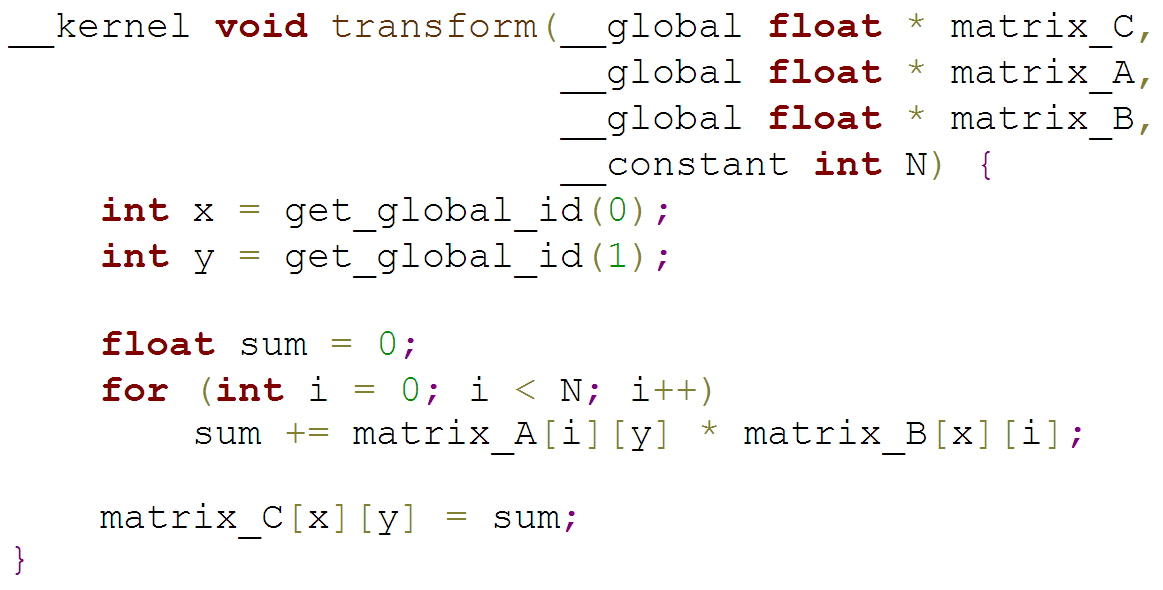
\includegraphics[height=0.27\textheight]{graphics/opencl_kernel.png}
		\caption{OpenCL matrix multiplication kernel}
		\label{fig:opencl_kernel}
		\end{figure}
	
	The OpenCL C-based programming language supports vector arithmetic with integer or floating point vectors of 2, 4, 8 and 16 elements. A number of built-in functions are provided for scalar and vector math, queries about \textit{NDRange} dimensions and work-item index, and for local or global synchronization. Some restrictions for use of the C99 standard apply, and these include: no recursion, use of \texttt{stdio} routines or external variables.

\chapter{Fast Reconstruction on the GPU}
	\label{chapter:gpu_reconstruction}
	
	% Repeat the motivation for the work
% Summarize what was done
% ? Explain why all goals have been met?

Ultrasound is a non-invasive, safe, low cost and practical way to provide medical doctors with an internal view of a patient's body. By performing 3D ultrasound reconstruction, 3D volumes can be constructed from 2D ultrasound scans, and be used for acquiring out-of-angle views, 3D rendering of the anatomy, and for image guided surgery. The purpose of this thesis was to investigate the parallel processing power of the GPU for fast ultrasound reconstruction. Having the ability to reconstruct a volume in a fraction of a second enables instant feedback and real-time incremental reconstruction while scanning. This thesis has presented our techniques to perform fast, non-incremental and real-time incremental reconstruction using the GPU. Optimization techniques for both pixel-based and voxel-based approaches have been described, and a novel method of doing real-time incremental reconstruction was presented. The performance obtained by these methods have been measured on some of the latest hardware architectures at the time of writing from both Nvidia and AMD. Issues for future work to look into are suggested in Section \ref{section:future_work}, and some final thoughts and closing statements are also given in Section \ref{section:final_thoughts}.
	
	\section{Preprocessing of Input Data}
	
		% description of input interpolation and calibration
		% intro
For both pixel-based and voxel-based reconstruction, the input data is processed before the actual reconstruction. In our case, this means calibrating the tracking data and handling the different rate of tracking data and ultrasound scans.

% why this is necessary and how it is done
\subsection{Calibration of Tracking Data}

	\begin{figure}[h]
	\centering
	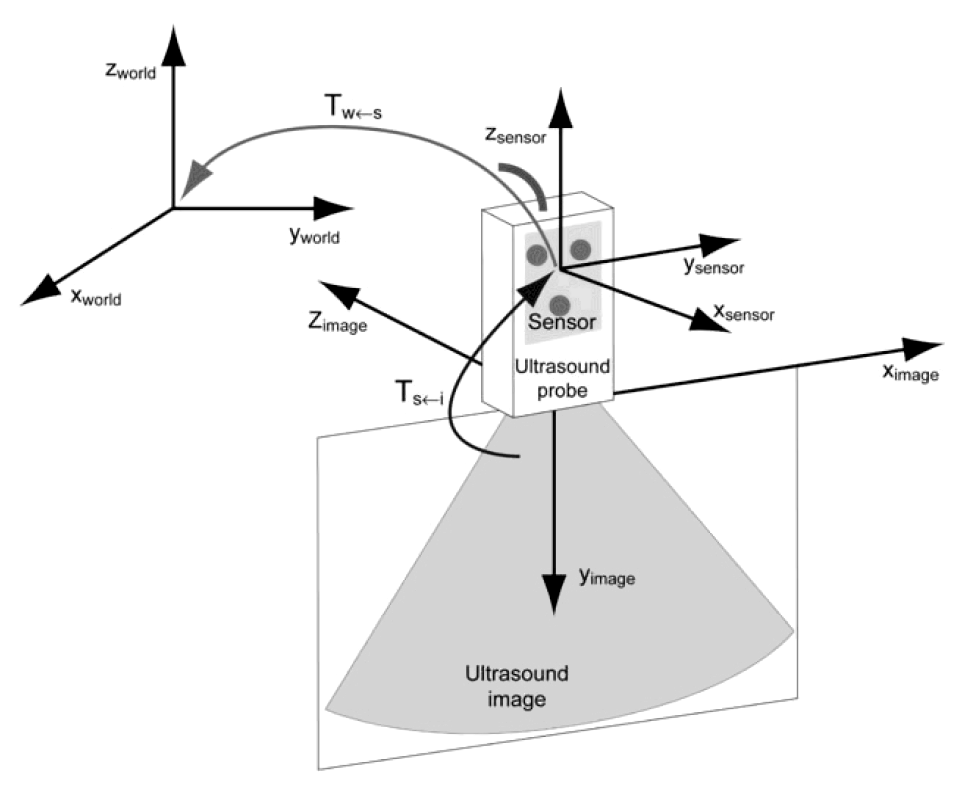
\includegraphics[width=\textwidth]{graphics/tracking_spaces.png}
	\caption[Spaces of a tracking system]{Spaces of a tracking system (used with permission from \cite{mercier2005})}
	\label{fig:tracking_spaces}
	\end{figure}

	Figure \ref{fig:tracking_spaces} shows a tracking system with a sensor attached to an ultrasound probe. The tracking system will give the relation between the sensor and the world space, $T_{w \leftarrow s}$, in the form of a transformation matrix. This transforms coordinates in the space of the sensor to coordinates in the world reference space. However, even though the sensor is tightly attached to the probe, it is not in the origin of the space of the ultrasound images. This relation, $T_{s \leftarrow i}$ varies with each tracking system's setup, so a calibration transformation is required and is part of the input. Before the reconstruction begins this calibration matrix is multiplied into the tracking transformations.

% what this problem is and how it is handled by interpolation
\subsection{Handling Different Tracking and Scanning Rate}

	While the probe catches ultrasound images, the tracking system outputs a series of transformation matrices. Ideally, the tracking system and ultrasound probe should be synchronized such that each b-scan has an associated transformation. However, the tracking system used in this thesis has a slighter higher rate than the probe.  Is is assumed that both systems start and stop at the same time. As an example, one of the input set used in this thesis has 434 b-scans and 520 tracked positions.
	
	This is handled by interpolating the tracking data stream between the b-scan stream. Since the tracking data consists of $4 \times 3$ matrices of floating point values, it is obviously easier to interpolate than the b-scans with thousands of pixels. Each b-scan and tracked position has an associated timetag, but the probe and tracking system use clocks with different timestamp resolutions.
	
	Given these considerations, the timetags are first normalized to the same unit by first subtracting the first timetag from all timetags in each stream respectively. In this manner, each stream begins with the time 0. Then, each tracking timetag is multiplied by the ratio between the last b-scan timetag and the last tracking timetag. This makes the tracking timetags end with the same timetag as the b-scan timetags.
	
	\begin{figure}[h]
	\centering
	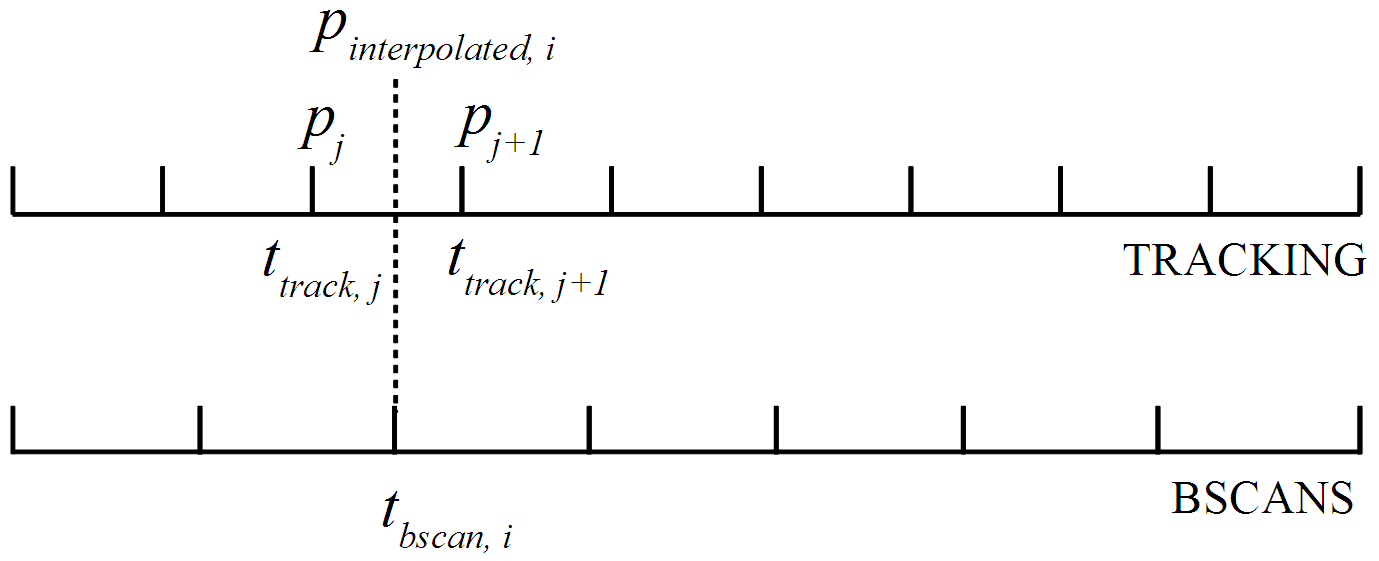
\includegraphics[width=\textwidth]{graphics/tracking_scanning_interpolation.png}
	\caption{Interpolation of tracking data after timetag normalization}
	\label{fig:tracking_scanning_interpolation}
	\end{figure}
	
	 Figure \ref{fig:tracking_scanning_interpolation} shows how the tracking data is interpolated using the normalized timetags. Each interpolated value is given by Equation \ref{eq:tracking_scanning_interpolation} where $p_{interpolated,i}$ is the value interpolated between $p_j$ and $p_{j+1}$ given the timetags $t_{bscan}$ and $t_{track}$ of the b-scans and tracking data. The values in the first and last tracking matrices need not be interpolated (because of tracking and scanning starting and stopping at the same time).
	 
	\begin{equation}
		p_{interpolated,i} = p_j + \frac{t_{bscan,i} - t_{track,j}}{t_{track,j+1} - t_{track,j}} \cdot (p_{j+1} - p_{j})
	\label{eq:tracking_scanning_interpolation}
	\end{equation}
	
	\section{Pixel-Based Reconstruction}
		\label{section:non-incremental_pnn}
	
		% description of how PNN reconstruction on the GPU was done in this thesis
		% intro
Pixel-based reconstruction is an intuitive method to construct a volume from oriented ultrasound scans. In abstract sense, the scans are simply "inserted" into the volume. However, for a computer to this, a series of algorithmic steps needs to be devised. To obtain high performance, we can parallelize this algorithm and optimize the implementation. This section explains how pixel-based reconstruction is done in this thesis, including how this is parallelized and optimized for the GPU.

% description of the steps
\subsection{Method}

% (Fill compressed mask from mask)
% Fill pixel_ill from b-scans and mask
% Fill pixel_pos from mask
% Transform pixel_pos by pos_matrices
% Convert pixel_pos to volume indices
% Fill volume from pixel_pos and pixel_ill
% Fill holes of volume

	The method is based on pixel-nearest-neighbor (PNN) \cite{mccann1988}. The input is a set of $n$ b-scans images, a mask defining a region of interest (ROI) and $n$ tracking matrices. The b-scans are $w \times h$ arrays of grey-scale intensities, with 1 byte per pixel ($2^8=256$ possible values). The mask is the same format, where black is outside the ROI and white is inside, but there is only 1 mask for all $n$ b-scans. The tracking matrices are interpolated and calibrated using the $4 \times 3$ floating point transformation matrices as described in the previous section. The bottom row in the matrices will always be $(0,0,0,1)$, and is omitted.
	
	\begin{figure}[h]
	\centering
	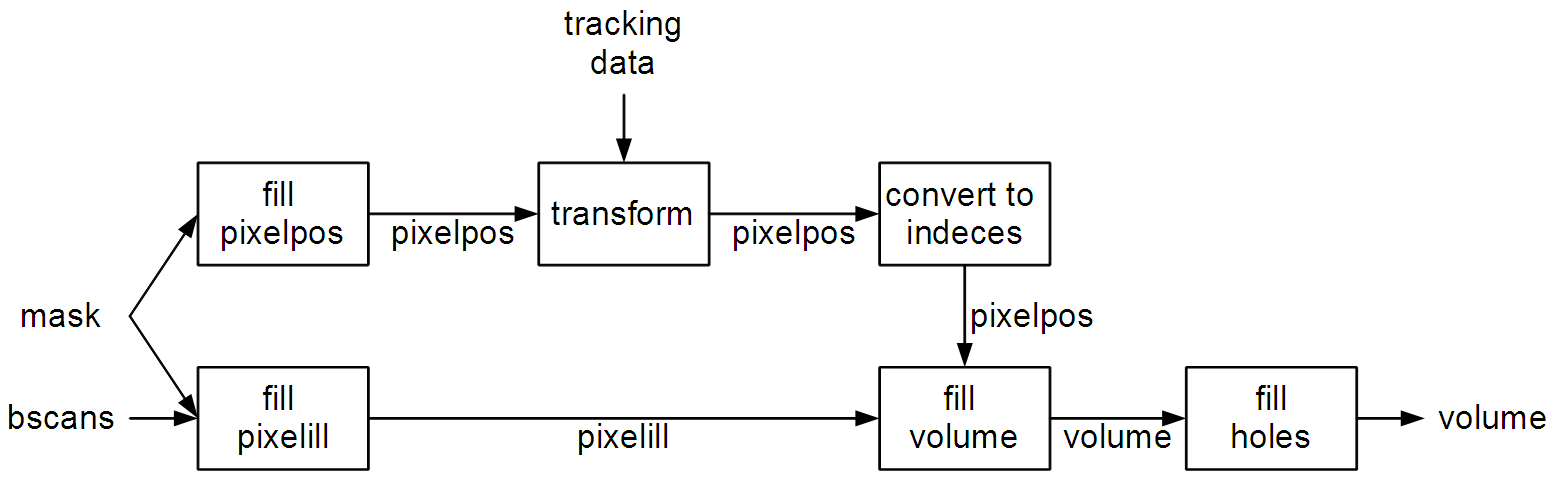
\includegraphics[width=\textwidth]{graphics/non-inc_pnn.png}
	\caption{Steps performed in pixel-based reconstruction}
	\label{fig:non-inc_pnn}
	\end{figure}
	
	There are 6 steps to be performed, resulting in the reconstructed volume. These steps are illustrated in Figure \ref{fig:non-inc_pnn} and given in the list below:
	
	\begin{enumerate}
		\item Fill $pixelpos$ from mask
		\item Fill $pixelill$ from b-scans and mask
		\item Transform $pixelpos$ by tracking matrices
		\item Convert coordinates to volume indices
		\item Fill volume from $pixelill$ and $pixelpos$
		\item Fill volume holes
	\end{enumerate}
	
	In the first step, we construct an array of three-dimensional coordinates, $pixelpos$, with one position for each pixel that is in the ROI in the mask. The coordinates are in world space, and are such that all the b-scans lie flat on the YZ-plane. This is given by Equation \ref{eq:pixelpos} where $i$ is the b-scan index (disregarded), $x$ and $y$ are the pixel indices, and $\Delta x$ and $\Delta y$ are the spacings between pixels in x- and y-direction (given as part of input). These coordinates are to be rotated by the tracking matrices to be positioned in the volume.
	
	\begin{equation}
	\label{eq:pixelpos}
		pixelpos(i,x,y) = (0, x\Delta x, y\Delta y)
	\end{equation}
	
	In the second step, the grey-scale intensities of the pixels in the ROI are saved as an array of bytes. The reason for doing this apparently redundant work is that the ROI can be much smaller than the entire b-scan. Typically, the scans are captured by a frame-grabber card connected to the ultrasound machine, and these images include metadata and empty space around the actual ultrasound data. The ROI is then just a fraction of the entire image. As an example, in the test data used in this thesis the ROI is 28 \% of the full scan. By extracting these into a separate array, we save memory, and there is a practical one-to-one mapping between pixel coordinates and pixel intensities.
	
	With this data ready, the transformation can begin in step three. For each b-scan, the corresponding tracking matrix is multiplied with the pixel coordinates to yield the coordinates in the volume. The operation is shown in Equation \ref{eq:transform_pixel_pos}. These coordinates are in world space, and in step four these are converted to volume indices by Equation \ref{eq:round_off} where $\Delta v$ is a given spacing between neighbor voxels. With the transformed coordinates converted to volume indices, the volume can be populated in step five. For each of the processed pixel coordinates, their corresponding pixel intensity is inserted into the volume using one of the possible compounding methods given in Table \ref{table:compounding_methods}. The effect of each specific method is given as an expression of the $old$ value present in the voxel and the $new$ value to be inserted.
	
	\begin{equation}
	\label{eq:transform_pixel_pos}
		pixelpos(i,x,y) := \bb{T}_i \cdot pixelpos(i,x,y)
	\end{equation}
	
	\begin{equation}
	\label{eq:round_off}
		pixelpos(i,x,y) := \Delta v \cdot pixelpos(i,x,y)
	\end{equation}
	
	\begin{table}[h]
	\centering
	\begin{tabular}{| l l l |}
		\hline
		\multicolumn{1}{|c}{\textbf{Method}} & \multicolumn{1}{c}{\textbf{Effect}} & \multicolumn{1}{c|}{\textbf{Condition}} \\
		\hline
		\hline
		average 			& $voxel \leftarrow \frac{old+new}{2}$ 	& old is not empty \\
		average 			& $voxel \leftarrow new$ 				& old is empty \\
		max 				& $voxel \leftarrow max(old, new)$ 		& \\
		ifempty 			& $voxel \leftarrow new$ 				& old is empty \\
		ifempty 			& $voxel \leftarrow old$ 				& old is not empty \\
		overwrite 			& $voxel \leftarrow new$ 				& \\
		\hline
	\end{tabular}
	\caption{Compounding methods}
	\label{table:compounding_methods}
	\end{table}
	
	The sixth and final step is to fill the volume holes. For each empty voxel, a $k \times k \times k$ kernel around it is averaged to give the voxel a value. In this kernel, only the non-empty voxels are considered for calculating the average, otherwise the filled holes would be darker than the surroundings. To save memory, hole filling is done in place, and thus there is a need for differentiating between actual holes and the empty voxel values before the first and after the last b-scan, in addition to those outside the region-of-interest. If every empty voxel would simply be filled, then non-empty voxels at the edges would be smudged out in the empty regions. This is resolved by counting the number of empty voxels in the kernel, and then only using the average to fill the hole if this number is above a cutoff value. An example cutoff value is $(k^3/2)-k$, which is slightly lower than half the number of voxels in the kernel. If the holes are not filled in place, e.g.\ by using a separate copy of the volume that has its holes filled, this cutoff is not necessary.

% description of how data/work is split up for parallelization,
% and also what parts are done on the CPU and GPU
\subsection{Parallelization}

%	Best practices guide p 31: multidimensional aspect of grid does not play a role in performance
%	Process input done on CPU because negligible
%	transfer b-scans and mask
%	?Generating pixel_pos and pixel_ill on GPU instead of transfer
%	NDRanges:
		%fill_pixel_ill_pos 	b-scan_n
		%transform 				b-scan_n x mask_size
		%round_off_translate	b-scan_n x mask_size
		%fill_volume			b-scan_n x mask_size
		%fill_holes				volume_w x volume_h x volume_n
%	Split b-scans and pixel_pos to overcome memory limits
%	transfer volume to CPU after processing

Code listings of the implemented OpenCL kernels can be found in Appendix \ref{section:pnn_kernel}. To parallelize the pixel-based reconstruction on the GPU, we need to divide the work into parts that can be performed simultaneously by many threads. To fully utilize the GPU, the number of work-items should in the order of hundreds of thousands or even millions \cite{bestpractices}. An elegant split of the work-domain will also ease the design of the kernels. OpenCL supports an \textit{NDRange} of up to three dimensions, but this multidimensional aspect does not play a role in overall performance \cite{bestpractices}, so this is not a consideration here.

Another task when parallelizing is to decide what parts to run on the highly parallel GPU and what parts to run on the relatively sequential CPU. There are additional overheads associated with doing work on the GPU, such as transferring data to and from the device memory and launching the kernel. The task of processing the input by calibration and interpolation is too small to be worth parallelizing for the GPU. However, each step in the reconstruction is parallelized.

After the input b-scans and tracking data has been transferred to the GPU memory, $pixelpos$ and $pixelill$ are generated and stored on the device. These arrays are only needed intermittently during reconstruction and thus never need to be transferred to or from the GPU. There are $n \times w \times h$ pixels that need to be processed into $n \times m$ coordinates in $pixelpos$, and intensities in $pixelill$, where $m$ is the number of pixels in the ROI. Dividing this into $n \times w \times h$ work-items is problematic because each work-item does not know where in the $pixelpos$ and $pixelill$ buffers to write when they find a ROI pixel. The solution is to evaluate $m$ on the CPU (negligible computation time), and give this as parameter to $n$ work-items that process a b-scan each. Each thread should generate $m$ elements, so a private counter is sufficient to manage where to write in memory.

The next three steps will process the $n \times m$ elements of $pixelpos$ and $pixelill$. The transformation task is divided into $n \times m$ work-items that each perform one matrix multiplication. The task of converting the coordinates to voxel indices and using them to fill the volume has the same number of work-items. For clarity however, these steps are not merged into one kernel. Filling the volume holes, on the other hand, is independent of the size of the input. The massive parallelism of the GPU allows for creating one work-item per voxel, totaling possibly millions, and where each work-item averages the neighbors if the voxel is empty. After this step, the volume is transferred back from the device if so desired. If the volume is visualized while on the GPU, this step might be skipped to save the transfer time.

%While commodity computers typically have 2 or more gigabytes of memory, GPUs found in current computers\footnote{Apple Mac Pro (2010)} can have only 512 megabytes. Some of this memory must be used by other applications, and the maximum

% description of various tricks and optimizations done
\subsection{Optimization techniques}

%	Good work group sizes with padding (big and multiple of 32)
%	Reduce variables to lower register usage
%	Compressed mask in constant memory
%	Transformation matrix in constant memory
%	Using constant memory for non-pointer arguments

In addition to increased performance from processing elements in parallel, there are further optimizations that can be performed. Actually, a naive porting of sequential code to the GPU does not necessarily utilize the device's capabilities, and might even result in a \emph{slowdown}. To make sure that each processing element in the device is occupied with work, we need to devise suitable work group sizes. As each work group is processed on one compute unit, we also need to ensure that its resources (such as shared memory) are not exhausted. On the CUDA architecture, groups (\emph{warps} in CUDA terminology) of 32 work elements are processed at the same time, so work group size should\footnote{In fact, if not multiple of 32, they will be padded to be so by CUDA.} be a multiple of 32. In order to hide memory latency, the total number of work groups should also be such that each compute unit have multiple groups to manage. On the Nvidia Tesla C2050 GPU, there are 16 compute units.

For the task of filling $pixelpos$ and $pixelill$, the \textit{NDRange} is only $n$ work-items, which is typically 200-500. To ensure enough work groups, we use a work group size of 32 and pad the \textit{NDRange} to a multiple of this work size. Such padding is generally done by Equation \ref{eq:padding}, where $p$ is the value of what $n$ should be a multiple of. The next steps have a substantially higher \textit{NDRange}, and we use work groups of 512 work-items which is the maximum possible size.

\begin{equation}
	\label{eq:padding}
	n_{padded} = (\lfloor \frac{n}{p} \rfloor + 1) \cdot p
\end{equation}

For further optimizations, the number of variables in the code is manually reduced to lower register usage and small data buffers are put in fast constant memory. The transformation matrices are small enough to fit without modifications, and by compressing the mask it too can fit. As mentioned, the mask uses the same format as the b-scans, with one byte per pixel. As the ROI is a boolean value (either in or out), eight pixels can be encoded into one byte using bitwise operations. This compression is performed on the CPU and also makes the mask faster to transfer to the device's memory.
	
	\section{Voxel-Based Reconstruction}
		\label{section:non-incremental_vnn}
	
		% description of how VNN reconstruction on the GPU was done in this thesis
		% intro
Performing voxel-based (or "backwards") reconstruction is not as straight forward as the pixel-based method. For each voxel, one must find the b-scan that is closest when transformed into the volume. When found, the pixel on this b-scan that will contribute to the voxel must then be located. In this section, the voxel-based reconstruction implemented in this thesis is described. As in the previous section on pixel-based reconstruction, we also cover how this is parallelized on the GPU and some of the important optimization techniques.

% description of the steps
\subsection{Method}

%	(interpolate and calibrate)
%	fill plane_points
%	transform plane_points
%	fill b-scan_plane_equations from plane_points
%	for each voxel:
	%	calculate distance to planes, find smallest distance
	%	use plane normal and distance to get projected point
	%	subtract corner0 and project on x- and y-vector to get 2D coordinates
	%	divide by b-scan spacing to convert to pixel indices
	%	fill voxel with pixel intensity using compounding methods
	
The method is based on voxel-nearest-neighbor (VNN) \cite{sherebrin1996}. As with pixel-based reconstruction, the input tracking data must be calibrated and interpolated. After this has been completed, the two approaches start differ. The reconstruction consists of the following steps illustrated in Figure \ref{fig:non-inc_vnn}.

	\begin{figure}[h]
	\centering
	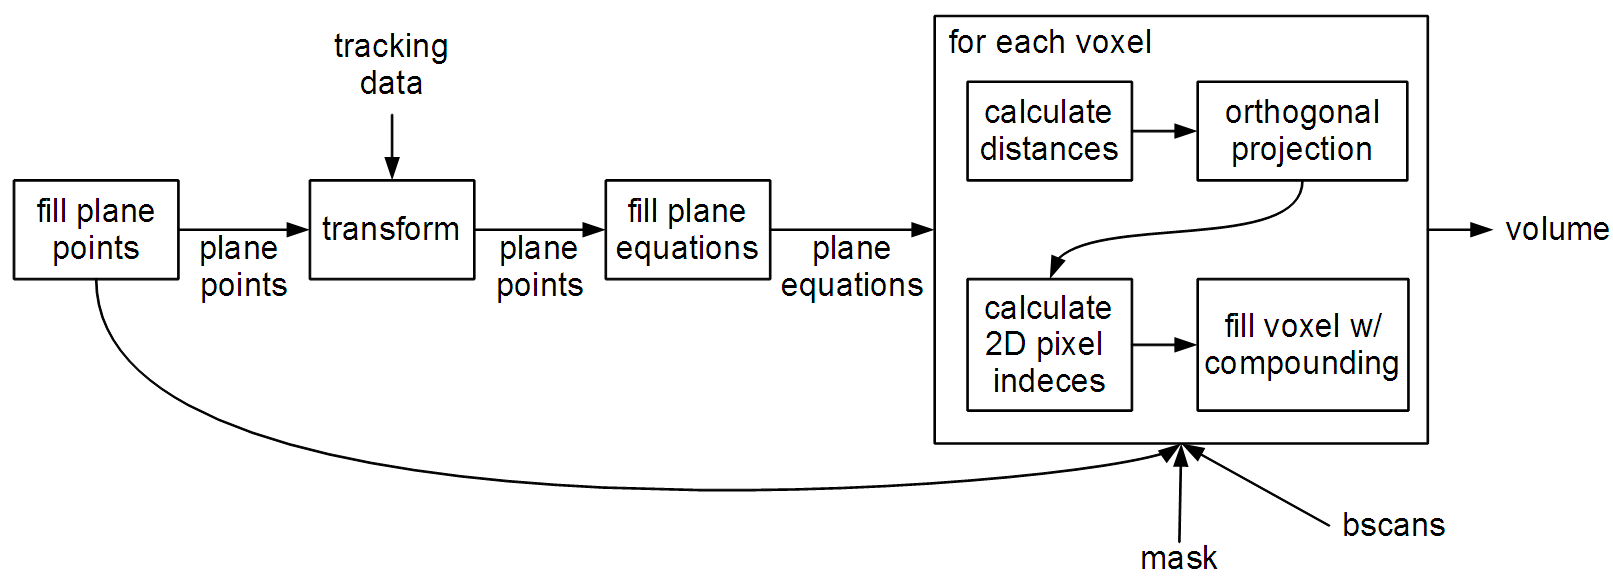
\includegraphics[width=\textwidth]{graphics/non-inc_vnn.png}
	\caption{Steps performed in voxel-based reconstruction}
	\label{fig:non-inc_vnn}
	\end{figure}

\begin{enumerate}
	\item Fill $planepoints$
	\item Transform $planepoints$
	\item Fill $planeequations$ from transformed $planepoints$
	\item For each voxel:
	\begin{enumerate}
		\item Calculate distance from voxel to planes
		\item Calculate orthogonal projection of voxel on closest plane
		\item Calculate 2D coordinates of projection on plane and convert to pixel indices
		\item Fill voxel using compounding methods
	\end{enumerate}
\end{enumerate}

In the first step an array of $n$ triplets of 3D space locations is constructed. The points in the triplet are the top-left, bottom-left and top-right corners of the b-scans in world coordinate space such that all b-scans are parallel and lie flat on the YZ plane. See Equation \ref{eq:plane_points}. The top-left corner is dubbed $corner0$, the top-right $cornerx$ and the bottom-left $cornery$.

\begin{equation}
\label{eq:plane_points}
	corner0 = (0,0,0), \; cornerx = (0,w\Delta x,0), \; cornery = (0,0,h\Delta y)
\end{equation}

In the second step, these points are transformed according to the tracking data. The transformation matrix of each b-scan is multiplied by each of the three corners, and the resulting coordinates are now correctly placed in world space. Three points is enough to define a plane, but to avoid redundant calculations, an array of $n$ plane equations is constructed in step three. Equations \ref{eq:pp2pe0} and \ref{eq:pp2pe1} show how three b-scan corners are used to calculate the parameters of a plane equation. Each plane equation has four parameters, $A$, $B$, $C$ and $D$, and define a plane implicitly. The plane equation is given in Equation \ref{eq:plane_equation}. The mathematically inclined reader will notice that A, B and C are vector coordinates of the plane normal, and D is the distance from origin to the closest point on the plane.

\begin{equation}
\label{eq:pp2pe0}
	normal = \frac{(corner0-cornerx) \times (cornery-corner0)}{|(corner0-cornerx) \times (cornery-corner0)|}
\end{equation}

\begin{equation}
\label{eq:pp2pe1}
	(A,B,C,D) = (normal_x, normal_y, normal_z, -A\cdot normal)
\end{equation}

\begin{equation}
\label{eq:plane_equation}
	Ax + By + Cz + D = 0
\end{equation}

The last step is to iterate over all voxels and fill their value from the closest b-scan. It is for this purpose that $planepoints$ and $planeequations$ were constructed in the previous steps. To fill a voxel, a series of \emph{substeps} are performed (see previous list). Each voxel with indices $(x,y,z)$ has world space coordinates given by $v = (x\Delta v,y\Delta v,z\Delta v)$. In the first substep (a), we calculate the distance of an orthogonal projection from these coordinates to each of the b-scan planes and find the minimum. The brute force approach is to test all planes, but a clever optimization technique has been devised and will be explained under "Optimization Techniques" below. For a point $v$, the orthogonal distance to a plane is found using Equation \ref{eq:distance}.

\begin{equation}
\label{eq:distance}
	distance = \frac{(A,B,C)\cdot v + D}{|(A,B,C)|}
\end{equation}

The next substep (b) is then to calculate the world space coordinates $p$ of the voxel coordinates orthogonally projected onto the plane. Given the distance and the plane normal, this is given as Equation \ref{eq:p}.

\begin{equation}
\label{eq:p}
	p = v - distance\cdot (A,B,C)
\end{equation}

To fill the voxel, we need the pixel intensity at this location ($p$) on the b-scan. This requires calculating the pixel indices in the b-scan image. To do this, substep (c), the vector from the top-left corner ($corner0$) to the point $p$ is projected onto normalized vectors parallel with the x and y axis of the b-scan. The lengths of the projections are divided by $\Delta x$ and $\Delta y$ to give pixel indices $(px,py)$. Equations \ref{eq:pxy0} and \ref{eq:pxy1} show the calculations.

\begin{equation}
\label{eq:pxy0}
	px = \frac{(p-corner0) \cdot |cornerx-corner0|}{\Delta x}
\end{equation}

\begin{equation}
\label{eq:pxy1}
	py = \frac{(p-corner0) \cdot |cornery-corner0|}{\Delta y}
\end{equation}

Given the indices of the contributing pixel, the last substep (d) is to fill the voxel with the calculated value.

% description of how data/work is split up for parallelization,
% and also what parts are done on the CPU and GPU
\subsection{Parallelization}

% All except voxel filling step done on CPU
% NDRange of volume_w x volume_n to utilize modified fast slice selection
% work group size of 512

A code listing of the implemented OpenCL kernel can be found in Appendix \ref{section:vnn_kernel}. In the previously described method, only step 4 is computationally demanding enough to require parallelization. There are only three points and one equation per input b-scan, and as there are typically around 200-500 such b-scans, the total computation time is negligible compared to iterating over all the voxels. For example, volume size can typically be $256^3$ or $512^3$. Also, the sizes of the corner points and equation parameters are small enough to be quickly transferred to the device. To summarize, step 1 to 3 is performed on the CPU, and step 4 is parallelized on the GPU.

The voxels are processed concurrently in columns. A volume of $w_{volume} \times h_{volume} \times n_{volume}$ voxels will result in $w_{volume} \times n_{volume}$ threads. Each thread executes a kernel that iterates over $h_{volume}$ voxels, performing substep (a) to (d) on each to fill them. The reason for this separation is that each voxel processed in a column is not more than than $\Delta v$ from the previously processed voxel, and this property is used in an optimization technique to be described below.

% description of various tricks and optimizations done
\subsection{Optimization Techniques}

%	NDRange optimizations
%	Modified fast slice selection!
	%	Process voxels in columns
	%	Search all planes for closest to first voxel in column
	%	for each voxel in column:
		%	"annenhver utover" from last closest plane
		%	break when difference between closest and current plane is above cutoff (it has peaked)
		
	During voxel-based reconstruction, one of the most computationally demanding tasks is to find the b-scan that is closest to a voxel. The brute force approach involves testing all $n$ b-scans for each of the $w_{volume} \times h_{volume} \times n_{volume}$ voxels, a computationally expensive task. However, it is possible to exploit inherent continuity in the b-scans.
	
	% Wein \textit{et al.}\ \cite{wein2006} describe a fast way to decide the closest b-scan, by iterating over the voxels in a pattern such that each processed voxel is next to the previously processed voxel. 
	
	Ideally, each b-scan will come "after" the previous one. In other words no b-scan will intersect another, and each b-scan is in front of the previous (in the direction of the probe's trajectory). Noise in the tracking data and an unsteady hand can cause the b-scans to be partially shuffled. Additionally, when rotating the probe, there is a high probability that b-scans will intersect each other. Even though the b-scans may come in any order, the general tendency is along the probe trajectory. In other words, they are \emph{partially ordered}. This means that if the closest b-scan to a given voxel is found, then the index of the closest b-scan to the neighbor voxel is probably close to the index of the previously closest b-scan. To take advantage of this, the following scheme was devised:
	
	\begin{itemize}
		\item Let each thread process a column of voxels
		\item $i$ = index of b-scan closest to first voxel in column found by brute force
		\item For each voxel in column:
		\begin{itemize}
			\item Loop $j \in {0, 1, 2, ..., n}$
			\begin{itemize}
				\item Calculate distance to b-scans with index $k=i+j$ and $l=i-j$ (if they exist)
				\item $i$ = the closest b-scan of $i$, $k$ and $l$
				\item If difference between distance to $i$ and distance to $k$ or $l$ is above a given cutoff, stop testing any more $k$s or $l$s, respectively
			\end{itemize}
		\end{itemize}
	\end{itemize}
	
	The idea is that b-scans before and after the previous b-scan that was closest are tested. It is important to process voxels next to each other and not, for instance, jump from voxel $(w-1,y,z)$ to $(0,y+1,z)$ because they are neighbors in memory. Since the b-scans are partially ordered the assumption is that when testing a  b-scan with an index far enough from the last b-scan that was closest, it will not be a better (closer) choice than the b-scans tested so far. The cutoff limit will depend on the nature of the input tracking data. For example, in one of our test cases, a cutoff of $4\Delta v$ was sufficient. After this, the distances found had "peaked", and the search could end.
	
\chapter{Real-Time Incremental Reconstruction and Visualization}
	\label{chapter:incremental_reconstruction_visualization}
	
	% Repeat the motivation for the work
% Summarize what was done
% ? Explain why all goals have been met?

Ultrasound is a non-invasive, safe, low cost and practical way to provide medical doctors with an internal view of a patient's body. By performing 3D ultrasound reconstruction, 3D volumes can be constructed from 2D ultrasound scans, and be used for acquiring out-of-angle views, 3D rendering of the anatomy, and for image guided surgery. The purpose of this thesis was to investigate the parallel processing power of the GPU for fast ultrasound reconstruction. Having the ability to reconstruct a volume in a fraction of a second enables instant feedback and real-time incremental reconstruction while scanning. This thesis has presented our techniques to perform fast, non-incremental and real-time incremental reconstruction using the GPU. Optimization techniques for both pixel-based and voxel-based approaches have been described, and a novel method of doing real-time incremental reconstruction was presented. The performance obtained by these methods have been measured on some of the latest hardware architectures at the time of writing from both Nvidia and AMD. Issues for future work to look into are suggested in Section \ref{section:future_work}, and some final thoughts and closing statements are also given in Section \ref{section:final_thoughts}.
	
	\section{Incremental Acquisition and Preprocessing of Input data}
		
		% description of waiting for b-scan and tracking data and interpolating the latter, plus calibration
		% Polling interface and retrieval algorithm
% Interpolating to match timetag and then calibration

When reconstructing incrementally, a method is needed for acquiring the b-scans from the ultrasound device (typically from a frame-grabber card) and the tracking data from the tracking system. This thesis does not focus on what goes on behind the scenes before this data is available in the computer's memory, but we define a simple interface that is assumed can be implemented by the ultrasound and tracking systems:

\begin{table}[h]
\centering
\begin{tabular}{| p{0.4\textwidth} p{0.5\textwidth} |}
	\hline
	\multicolumn{1}{|c}{\textbf{Call}} & \multicolumn{1}{c|}{\textbf{Effect}} \\
	\hline
	\hline
	\texttt{get\_last\_b-scan(timetag, b-scan)} & returns most recent b-scan and associated timetag \\
	\texttt{get\_last\_tracking(timetag, matrix)} & returns most recent tracking data in form of transformation matrix and associated timetag \\
	\texttt{poll\_b-scan} / \texttt{poll\_tracking} & returns true (once) when new b-scan/tracking data is ready, and false at each call after that until another b-scan/tracking data is ready \\
	\texttt{end\_of\_data} & returns true if there are no more b-scans \emph{or} no more tracking data to be expected (i.e. system turned off), false otherwise \\
	\hline
\end{tabular}
\caption{Interface against ultrasound and tracking system}
\label{table:ultrasound_interface}
\end{table}

Given this interface, the following algorithm is used for acquiring and processing the input data incrementally:

\begin{itemize}
	\item loop:
	\begin{enumerate}
		\item b-scan = NULL
		\item matrix = NULL
		\item while (matrix or b-scan is NULL)
		\begin{enumerate}
			\item if (\texttt{poll\_b-scan}) \texttt{get\_last\_b-scan(timetag\_b, b-scan)}
			\item if (\texttt{poll\_tracking}) \texttt{get\_last\_tracking(timetag\_m, matrix)}
		\end{enumerate}
		\item if (\texttt{end\_of\_data}) break loop
		\item interpolate tracking data and calibrate
		\item perform reconstruction increment
	\end{enumerate}
\end{itemize}

The reason for doing it in this fashion is that the rate of b-scan generation is not the same as the rate of incoming tracking data. After the while-loop in the algorithm has been completed, there has been acquired a b-scan and tracking data, but the tracking data is either from before or after the b-scan. As in the non-incremental method, we choose to interpolate the transformation matrix according to the given timetags. This, together with the calibration, make up the preprocessing of the input data. After this step, one increment of the reconstruction can be performed.
	
	\section{Incremental PNN Reconstruction}
	
		% description of how simple PNN is performed incrementally in real-time on the GPU
		%intro
The pixel-nearest-neighbor (PNN) method is suitable for incremental reconstruction as each incoming b-scan can be processed and put into the volume. Since pixel-based methods work forward, only the voxels affected by a b-scan are processed. In contrast, voxel-based methods work backwards, and all voxels must be processed for each increment of the reconstruction.

In this section, we describe how to perform incremental PNN reconstruction utilizing the GPU for parallel processing. In the incremental algorithm, not all steps benefit from being offloaded to the GPU, and the distribution between CPU and GPU is covered here. Although PNN is suitable for incremental reconstruction, the hole-filling stage introduces difficulties when trying to maintain high performance. This will also be explained, and some possible solutions are presented.

\subsection{Method and Parallelization}
% description of each step:
	% for each b-scan and tracking data:
		% fill pixel_ill and pixel_pos (CPU)
		% transfer pos_matrix, b-scan, pixel_ill and pixel_pos to GPU
		% transform pixel_pos (GPU)
		% convert pixel_pos to voxel indices (GPU)
		% fill volume in device memory (GPU)
		% transfer pixel_pos to CPU
		% fill volume in CPU memory (CPU)
% for each step, why on CPU/GPU
% before three last steps, epxlain why reconstruct volume on GPU and CPU instead of transferring

The method used for incremental PNN is similar to ordinary non-incremental PNN. This is why PNN was chosen for a simple incremental reconstruction method. For each increment, we assume that a b-scan and its interpolated and calibrated tracking transformation matrix has been acquired as described in the previous section. The steps are then as follows:

\begin{itemize}
	\item For each acquired b-scan and associated tracking data:
	\begin{enumerate}
		\item Fill $pixelill$ and $pixelpos$ (on CPU)
		\item Transfer b-scan, tracking data, $pixelill$ and $pixelpos$ to GPU
		\item Transform $pixelpos$ (on GPU)
		\item Convert $pixelpos$ to voxel indices (on GPU)
		\item Fill device memory volume (on GPU)
		\item Transfer $pixelpos$ to CPU
		\item Fill CPU memory volume (on CPU)
	\end{enumerate}
\end{itemize}

The main steps are the same as in the non-incremental version: fill $pixelill$ and $pixelpos$, transform, convert to voxel indices and fill the volume. However, in the incremental version some steps previously done on the GPU are now performed on the CPU, and in addition we maintain a duplicate volume on the CPU in addition to the GPU. The reason behind these differences will be explained below.

In step 1, the mask is used to fill $pixelill$ with pixel intensities and $pixelpos$ with untransformed coordinates, just like with non-incremental PNN, but this step is now performed on the CPU. The reason for this is that while it is straightforward to divide the work into one b-scan per thread, it is harder to divide the work of a single b-scan. As mentioned in Section \ref{section:non-incremental_pnn}, parallelizing the sequential code requires each thread to know where in the buffer to write the data if a pixel in the ROI is found. This could be performed with an atomic update of a global variable identifying the next position to write to, but the overhead of maintaining and waiting for this variable overshadows the benefits of parallelizing the task. This operation is fairly trivial, and takes negligible time when only processing a single b-scan. So although an atomic counter or other scheme for parallelizing this might achieve the same effect, the simplest solution is to perform this sequentially on the CPU and then transfer the results (of negligible size for single b-scan) to the device.

In contrast to step 1, transforming the coordinates in step 3 is a computationally heavy task and is best suited for the GPU, and the implementation is straight forward with $m$ threads (one for each pixel in the ROI). A typical mask has around 100 000 pixels, which is more than enough to occupy the compute units on a modern GPU. Again the same approach is used in step 4 where we parallelize using one thread per pixel in the ROI. As the data is already on the device memory, it is logical to perform this step on the GPU.

In non-incremental reconstruction, if the volume is not solely used for visualization on the GPU, it is transferred from device to host when the reconstruction is complete. To do the same incrementally would be a performance bottleneck as tens of megabytes of data would be transferred for each increment of the reconstruction. To reduce the bandwidth used, we transfer only the processed $pixelpos$ from device to host, and use the $pixelill$ (from step 1) that already exists on the host to fill a volume duplicate on CPU memory. This incrementally updated volume can be used in any third-party application. If the volume is only used for visualization on the GPU, then the two last steps may be omitted. It is also possible to visualize the volume on the GPU during reconstruction, and then transfer the whole volume to the CPU only at the end of the reconstruction session.

\subsection{Incremental Pixel-Based Hole Filling}
% about the difficulties with incremental PNN hole filling
% suggestion(s) for how to do this with pros and cons
%	transfer entire volume each increment
%	splatting
%	have holes on CPU and fill only on GPU, then transfer at end of session
%	transferring filled holes to host (predetermined)


It should be highlighted that hole filling is omitted in the method presented in the last section. In the non-incremental version, hole-filling can be performed after all b-scans have been inserted into the volume. This is a computationally heavy task if performed for each increment for the entire volume. In addition, transferring the entire volume with filled holes is unacceptable if real-time performance should be maintained. Thus, there are two problems to be solved: the first is how to find and fill holes incrementally without processing the entire volume each increment, and the second is how to incrementally maintain a reconstructed volume on the host without transferring the entire volume each time. We present possible schemes to solve this.

The first method is to use some sort of "splatting" technique where each pixel contributes to voxels in a "splat" around its nearest neighbor. The splats can be spherical in nature and decrease in intensity as distance to the center increases. If sphere diameter is greater or equal to the maximum separation between two b-scans, no holes will occur. To implement this in the GPU-based PNN reconstruction, the splats are filled on the CPU and GPU volumes in step 5 and 7. The disadvantages are increased computation time (on CPU and GPU) spent on filling splats and blurring of the output volume.

Another approach is to use the parallel processing power of the GPU to fill holes on device memory volume, but not to transfer any additional hole-filling information to the host. The GPU volume will then have filled holes while the CPU volume will not, and it (the GPU volume) can be used for intermediate visualization where holes are not critical. At the end of the session, the entire hole-free volume can be transferred to host. Although bandwidth is saved in this approach, full hole filling is time consuming when performed on each increment, even on the GPU.

% TODO: This should be explained much better, using much more text and some illustrations:

It should not be necessary to search for holes in the entire volume for each increment. Holes may occur when two b-scans are more than $\Delta v$ from each other when inserted in the volume, and no other b-scans occur between them. This can be exploited by searching for holes in an area close to each inserted b-scan. Assuming no holes wider than $q$ voxels, we can search each inserted b-scan for holes in the $q \times m$ voxels immediately next to the voxels filled by the b-scan. In this way, a much smaller subset of the volume is searched, and we always know the upper limit of how many holes are filled on each increment. The $q \times m$ voxels intensities can be transferred to host in addition to $pixelpos$. The locations of the voxels where holes are filled can be set to the opposite direction of the current probe trajectory, and can thus be calculated from $pixelpos$ and the tracking data without transferring more coordinates to the host.
	
	\section{High-Quality Incremental Reconstruction}
		\label{section:incremental_hq}
	
		% description how incremental high-quality reconstruction in real-time on the GPU is done
		%intro (motivation and outline)
% about pixel-based vs voxel-based for incremental reconstruction
While incremental reconstruction with PNN is fast, it has its shortcomings. Due to the simplicity of the algorithm, the quality of the reconstructed volume is not as good as can be obtained with voxel-based methods using interpolation. Furthermore, hole filling is problematic when aiming for real-time performance. What is desired is a method that have high hole-free reconstruction quality, that can preferably be adjusted for a quality-time tradeoff, and one that is suitable for incremental updates of the volume without processing all voxels.

Pixel-based methods have the advantage of processing only the voxels that is actually updated by each b-scan, but the simplest variants can have the problem of holes. More advanced voxel-based methods can offer high reconstruction quality without holes, but are unsuitable for incremental updates. The method presented in this section combines the advantages from both approaches. The steps taken will be explained, together with issues from implementation and parallelization of the method are also covered.

% description of steps in the algorithm (incl DW and PT)
\subsection{Method}

% steps:
	% find ray-plane intersections
		% construct rays along axis and perform ray-plane intersection calculations
		% convert intersections to volume indices
	% fill voxels between intersection indices
		% linear interpolation ("DW") \cite{trobaugh1994}
			% for each b-scan in window:
				% orthogonal project voxel on b-scan
				% bilinear interpolation of 4 pixels
				% weight by inverse distance
			% divide by sum of weights
		% PT \cite{coupe2005}
			% linearly interpolate timetags by orthogonal distance
			% cubic interpolate 4 plane equations by key function
			% convert voxel coordinates on virtual plane to pixel indices
			% bilinear interpolate of 4 pixels on each b-scan
			% weight by inverse distance and divice by sum of weights
		% compound

The essence of the method is to transform incoming b-scan planes into the volume, but also to only process voxels located \emph{between} b-scans. For the voxels processed, voxel-based interpolation methods can be used to fill their values. This is what is meant by combining the pixel- and voxel-based approaches (or rather, the forward and backward approaches). B-scans are processed forwardly into the volume, but instead of filling the volume directly from the pixels, voxels between inserted b-scans have their values interpolated from the surrounding b-scans.

	\begin{figure}[h]
	\centering
	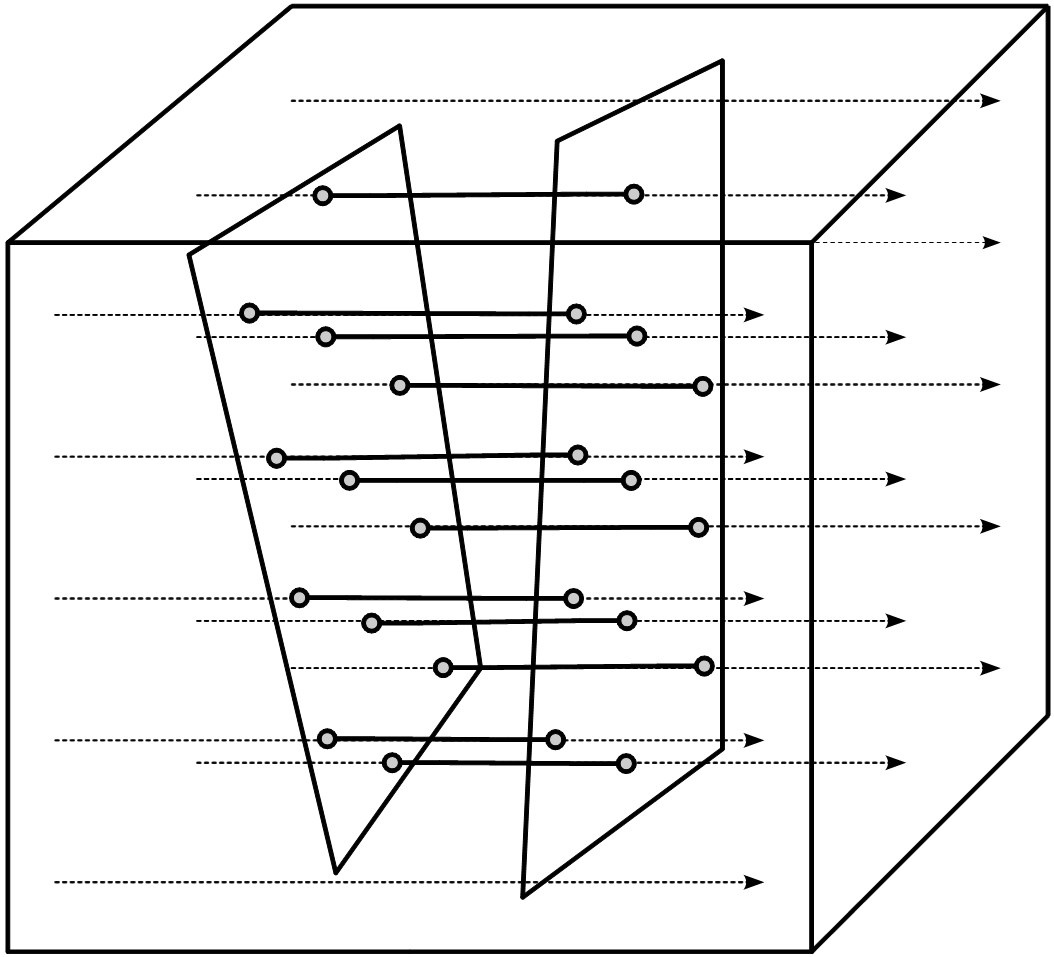
\includegraphics[height=0.4\textheight]{graphics/trace_intersections.png}
	\caption{Finding voxels between b-scans}
	\label{fig:trace_intersections}
	\end{figure}

For each incoming b-scan, we transform its corner points using the tracking data and construct its plane equation as previously described in Section \ref{section:non-incremental_vnn}. Figure \ref{fig:trace_intersections} show how the voxels between the current and previous b-scans are calculated. First, rays are constructed along columns of voxels, starting at the edge of the volume with one ray per column. These rays are used for ray-plane intersection calculations with the current and previous b-scan planes. The distance $t$ along a ray starting at $r_0$ with direction $r_d$ to a plane with equation parameters $(a,b,c,d)$ is given by Equation \ref{eq:ray-plane0}, and the voxel indices $(x,y,z)$ are given by Equation \ref{eq:ray-plane1}. Each ray gives one intersection point with the current b-scan, and another with the previous b-scan. The voxels between these will lie next to each other.

\begin{equation}
	\label{eq:ray-plane0}
	t = -\frac{(a,b,c) \cdot r_0 + d}{(a,b,c) \cdot r_d}
\end{equation}

\begin{equation}
	\label{eq:ray-plane1}
	(x,y,z) = \frac{r_0 + tr_d}{\Delta v}
\end{equation}

After the voxels between the b-scans have been found, they are each filled using a voxel based method. In our system, one can choose between two methods: one based on distance weighted orthogonal projections, and one based on cubic interpolation of the probe trajectory.

\subsubsection{Distance Weighted Orthogonal Projections}

	This method builds on the approach described by Trobaugh \textit{et al.}\ \cite{trobaugh1994}, where each voxel filled is orthogonally projected onto nearby b-scans and interpolated using the distance to the b-scan planes. But while Trobaugh \textit{et al.}\ project onto only two surrounding b-scans, we project onto the $n_w \leq n$ b-scans surrounding the voxel. The number of b-scans ($n_w$) taken into account for each voxel can be adjusted for a tradeoff between quality and performance. The 2D coordinates of the projected point on the b-scan plane can be found using equations previously described in Section \ref{section:non-incremental_vnn}. What differs, however, is that we project not only to the closest b-scan, but to all nearby b-scans. The number of b-scans used for each voxel increases the quality.  For each projection, the pixel intensity is given by a bilinear interpolation of the 4 pixels closest to the projected coordinates, as shown in Figure \ref{fig:bilinear} and given by Equation \ref{eq:bilinear_eq} where $x_f$ and $y_f$ is a fraction between 0.0 and 1.0 that says how far the projected point is from the closest pixel coordinates to the top-left. E.g.\ 0.5 means halfway between $(x,y)$ and $(x+1,y+1)$ (see figure). If one or more of the pixels are outside the ROI, the bilinear interpolated intensity is not used. Each intensity used is weighted by the inverse of the distance to the b-scan plane given by Equation \ref{eq:distance}. To normalize the result, it is divided by the sum of the weights as given by Equation \ref{eq:weighting}.
	
	\begin{figure}[h]
	\centering
	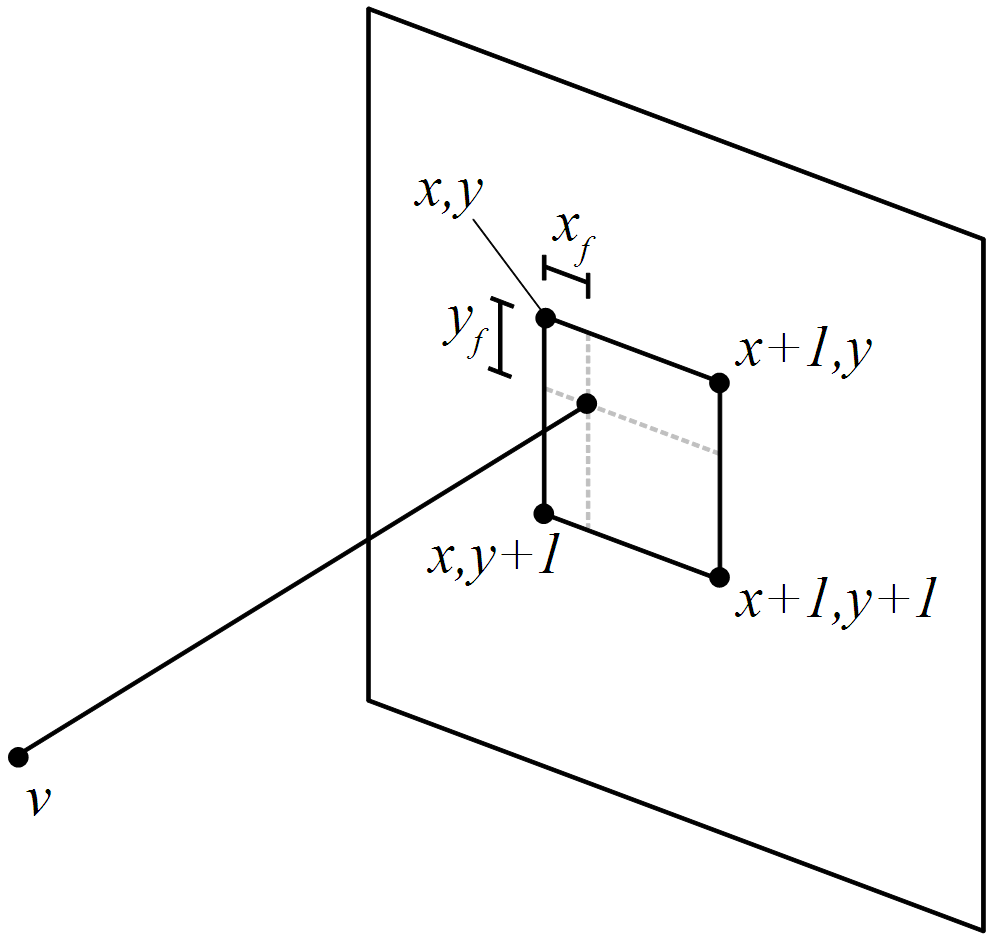
\includegraphics[height=0.35\textheight]{graphics/bilinear.png}
	\caption{Bilinear interpolation}
	\label{fig:bilinear}
	\end{figure}
	
	\begin{eqnarray}
		bilinear 	& = & b\-scan(x,y)(1-x_f)(1-y_f) + \nonumber \\
					&	& b\-scan(x+1,y) x_f (1-y_f) + \nonumber \\
					&	& b\-scan(x,y+1)(1-x_f) y_f + \nonumber \\
					&	& b\-scan(x+1,y+1) x_f y_f
		\label{eq:bilinear_eq}
	\end{eqnarray}
	
	\begin{equation}
		\label{eq:weighting}
		value_{dwop} = \frac{\sum_i (bilinear_i \cdot weight_i)}{\sum_i weight_i}
	\end{equation}
	
\subsubsection{Cubic Interpolation of Probe Trajectory}

	% linearly interpolate timetags by orthogonal distance
	% cubic interpolate 4 plane equations by key function
	% convert voxel coordinates on virtual plane to pixel indices
	% bilinear interpolate of 4 pixels on each b-scan
	% weight by inverse distance and divice by sum of weights
	
	This method is based on reconstruction as described by Coupe \textit{et al.}\ \cite{coupe2005}, but performed only on the voxels between two b-scans. The principle is to perform cubic interpolation of the tracking data as an estimation of the trajectory of the ultrasound probe. First, the timetags of two adjacent b-scans are linearly interpolated based on the orthogonal distance from the voxel coordinates in space to the b-scan planes, as illustrated in Figure \ref{fig:virtual_timetag} and given in Equation \ref{eq:virtual_timetag}. This new timetag is called a \emph{virtual timetag} and belongs to a virtual plane going through the voxel.
	
	\begin{figure}[h]
	\centering
	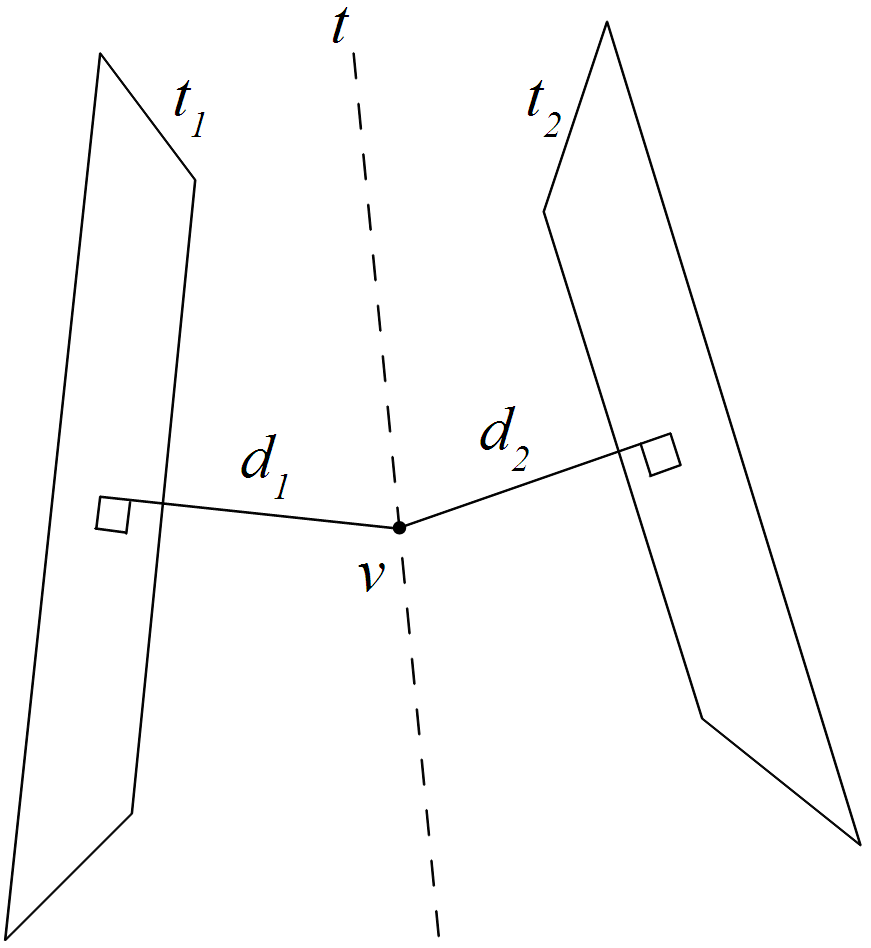
\includegraphics[height=0.35\textheight]{graphics/virtual_timetag.png}
	\caption{Timetag of virtual plane}
	\label{fig:virtual_timetag}
	\end{figure}
	
	\begin{equation}
		\label{eq:virtual_timetag}
		t = \frac{d_2 t_1}{d_1+d_2} + \frac{d_1 t_2}{d_1+d_2}
	\end{equation}
	
	To find the plane equation, top-left corner and x and y-vectors of the b-scan in the virtual plane, we use cubic interpolation based on the timetags through the \emph{key function} given in Equation \ref{eq:key_function} with $a = -\frac{1}{2}$. We interpolate plane equation parameters, corner and vector coordinates from four adjacent b-scans, where the two internal b-scans are those previously used to interpolate the virtual timetag. The cubic interpolation is shown in Figure \ref{fig:cubic_interpolation}. For each parameter or coordinate $\alpha$ to interpolate, the value of the key function is used in Equation \ref{eq:cubic_interpolation}.
	
	\begin{figure}[h]
	\centering
	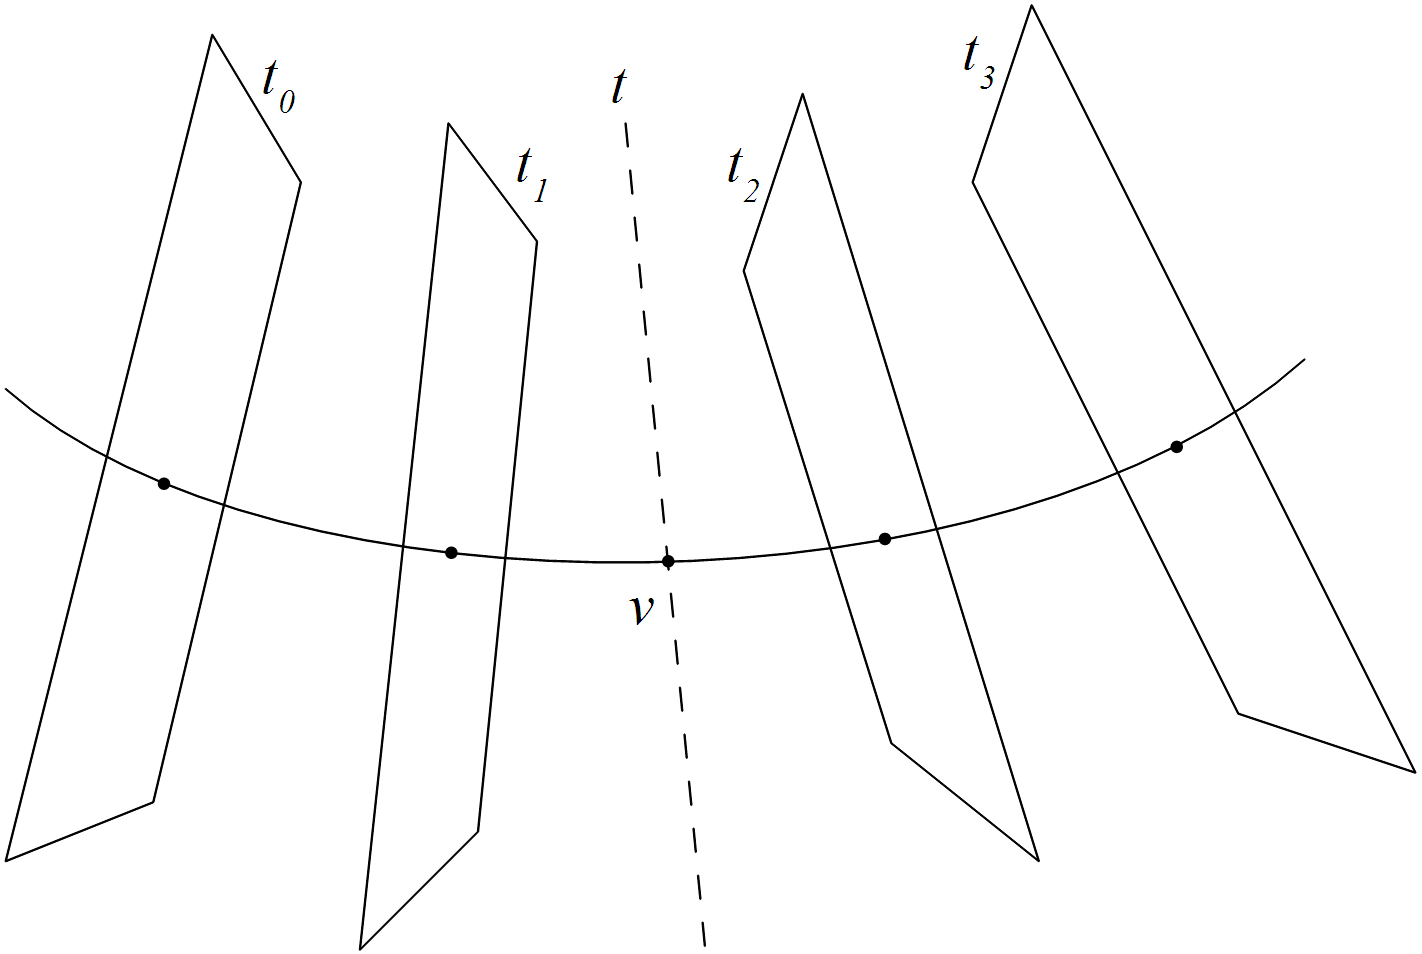
\includegraphics[height=0.35\textheight]{graphics/cubic_interpolation.png}
	\caption{Cubic interpolation of four b-scans}
	\label{fig:cubic_interpolation}
	\end{figure}
	
	\begin{equation}
		\label{eq:key_function}
		\phi(\beta) = \left\{ 
			\begin{array}{l l}
				(a+2)\beta^3 - (a+3)t^2 + 1 			& \quad \mbox{if $0 \leq \beta < 1$} \\
				a\beta^3 - 5a\beta^2 + 8a\beta - 4a 	& \quad \mbox{if $1 \leq \beta < 2$} \\
				0 										& \quad \mbox{if $2 \leq \beta$} \\
			\end{array}
		\right.
	\end{equation}
	
	\begin{equation}
		\label{eq:cubic_interpolation}
		\alpha = \sum_{i=0}^{4}\alpha_i \phi(\left|\frac{t-t_i}{t_1-t_0}\right|)
	\end{equation}
	
	When the virtual plane has been obtained, the 2D coordinates of the voxel (lying on the plane) can be found using the equations described in Section \ref{section:non-incremental_vnn}. These coordinates are then used on each of the four adjacent b-scans, and the pixels at those locations are bilinearly interpolated using Equation \ref{eq:bilinear_eq}. The four bilinearly interpolated values are then weighted by the inverse orthogonal distance to each b-scan from the voxel coordinates according to Equation \ref{eq:weighting}.

% description of how algorithm is implemented and parallelized
\subsection{Implementation and Parallelization}
	\label{section:incr_hq_impl}
	% queues and windows (options for plane a and b)
	% choose axis
	% restart if difference in timetags > cutoff
	% NDRange
	% CPU/GPU distribution
	
	Code listings of the implemented OpenCL kernels can be found in Appendix \ref{section:incremental_kernel}. To be able to interpolate between several b-scans, one solution is to queue up a buffer of incoming b-scans and tracking data. As incoming data is pushed into the queue, data is popped from the other end of the queue. When the session begins, the queue is simply filled without processing any of the input. During the session, this queue will be a "sliding window" across the stream of incoming data. The number of b-scans (each with associated tracking data) in the window is at least four if the probe trajectory (PT) method is used to fill the voxels, and a number $n_w \leq n$ if distance weighted orthogonal projections (DWOP) is used. There are several options for which two b-scan planes to use in the window when finding voxels to fill between them. To avoid repeated fillings of the same voxels, we use the planes of the two b-scans in the center of the window.
	
	When constructing the rays for the ray-plane intersection calculations, any axis can be used as a direction for the rays. As we parallelize with one thread per ray, we want to distribute work as evenly as possible. This means choosing an axis that is the most orthogonal to the normal for each b-scan. And by this we mean the axis that has the lowest angle between itself and the normalized b-scan plane normal $\bb{n}$ as given in Equation \ref{eq:axis}. The axis used is re-evaluated for each incoming b-scan.

\begin{equation}
	\label{eq:axis}
	S = \{(0,0,1), (0,1,0), (1,0,0)\}, \;\; ARGMIN_{\bb{a}\in S}(\bb{a} \cdot \bb{n})
\end{equation}

	To handle discontinuities in the input stream (e.g.\ from pauses in tracking during one session), a check is made for each incoming b-scan. If the increase in time according to the timetags is above a cutoff value, the reconstruction is restarted from that b-scan instead of attempting to interpolate across the discontinuity. Ultrasound systems usually have a regular acquisition rate $f$, and so a cutoff at $\frac{2}{f}$ is sufficient.
	
	As mentioned, the computations are parallelized with one thread per ray, and this \textit{NDRange} is kept as the voxels found by one ray will also be processed by the same thread. Assuming that the z-axis is always used as the best axis, the \textit{NDRange} will be $w \times h$ threads, each processing a number of voxels between 1 and the highest separation between two adjacent b-scans (typically $\leq 5$). 
	
	\section{Simultaneous Reconstruction and Visualization}
		\label{section:reconstruction_visualization}

		% description of how the volume was visualized, and how simultaneous recosntruction and visualization was done on the GPU
		%intro
One of the purposes of doing incremental reconstruction is to be able to see the volume as it is constructed. This allows for immediate feedback during scanning. There are many ways to visualize a volume, and the system described in this thesis offers orthogonal multiplanar reformatting (MPR) slices or volume ray casting. In addition, as the volume is accessible on both device and host memory, it can be used as input for third-party visualization packages. In this section, the visualization techniques used are described.

\subsection{Orthogonal MPR slices}
% pictchaz
% volume on CPU, slices extracted (no interpolation because of orthogonal along axis)
% how used OpenGL
% explain user interface (mouse rotate and index incr/decr)

\begin{figure}[h]
\centering
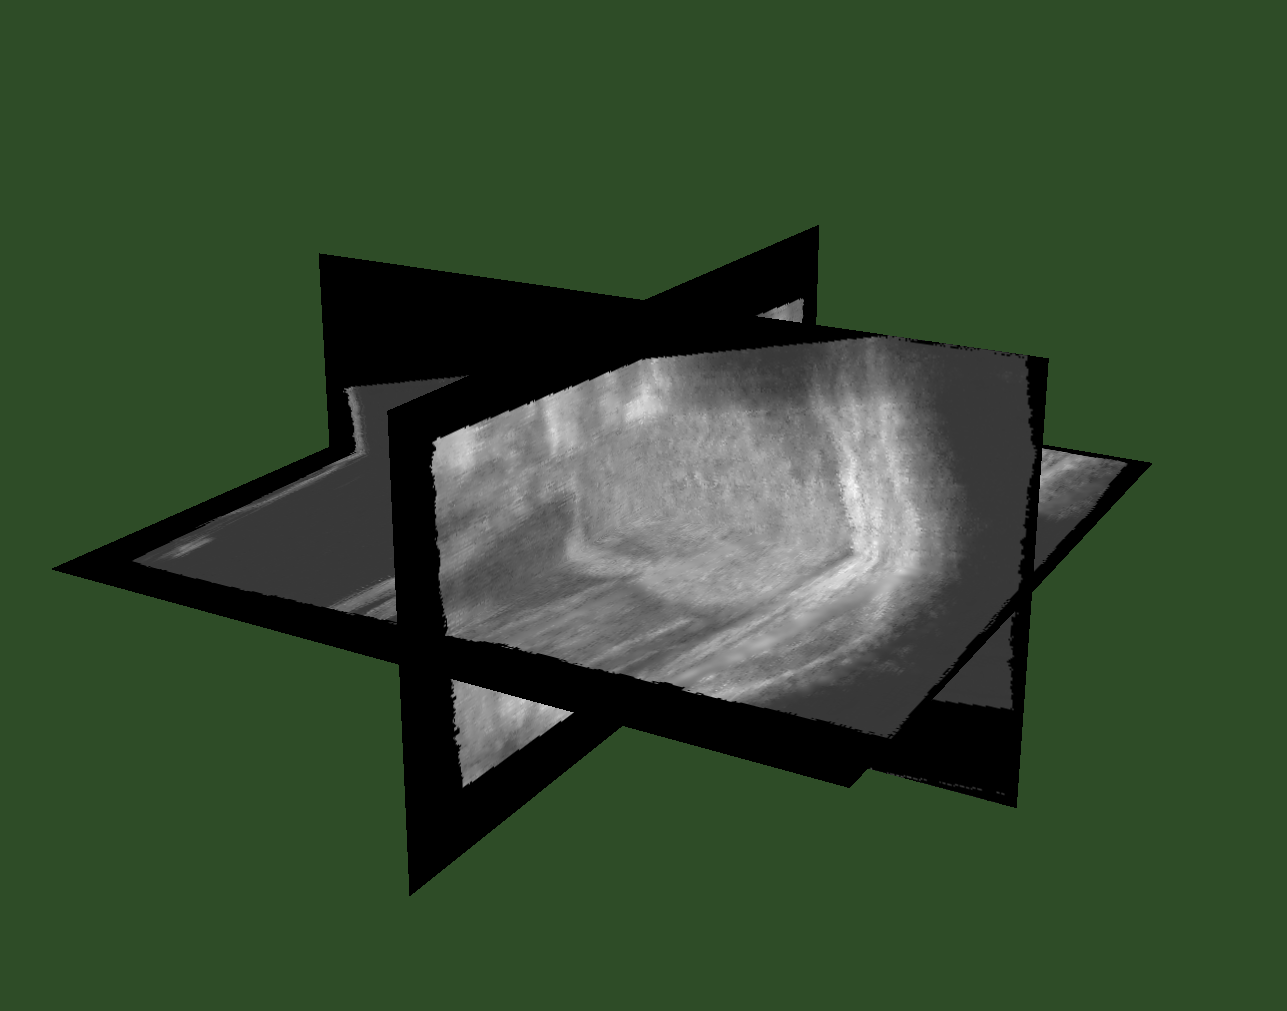
\includegraphics[width=0.49\textwidth]{graphics/orthogonal_screen0.png}
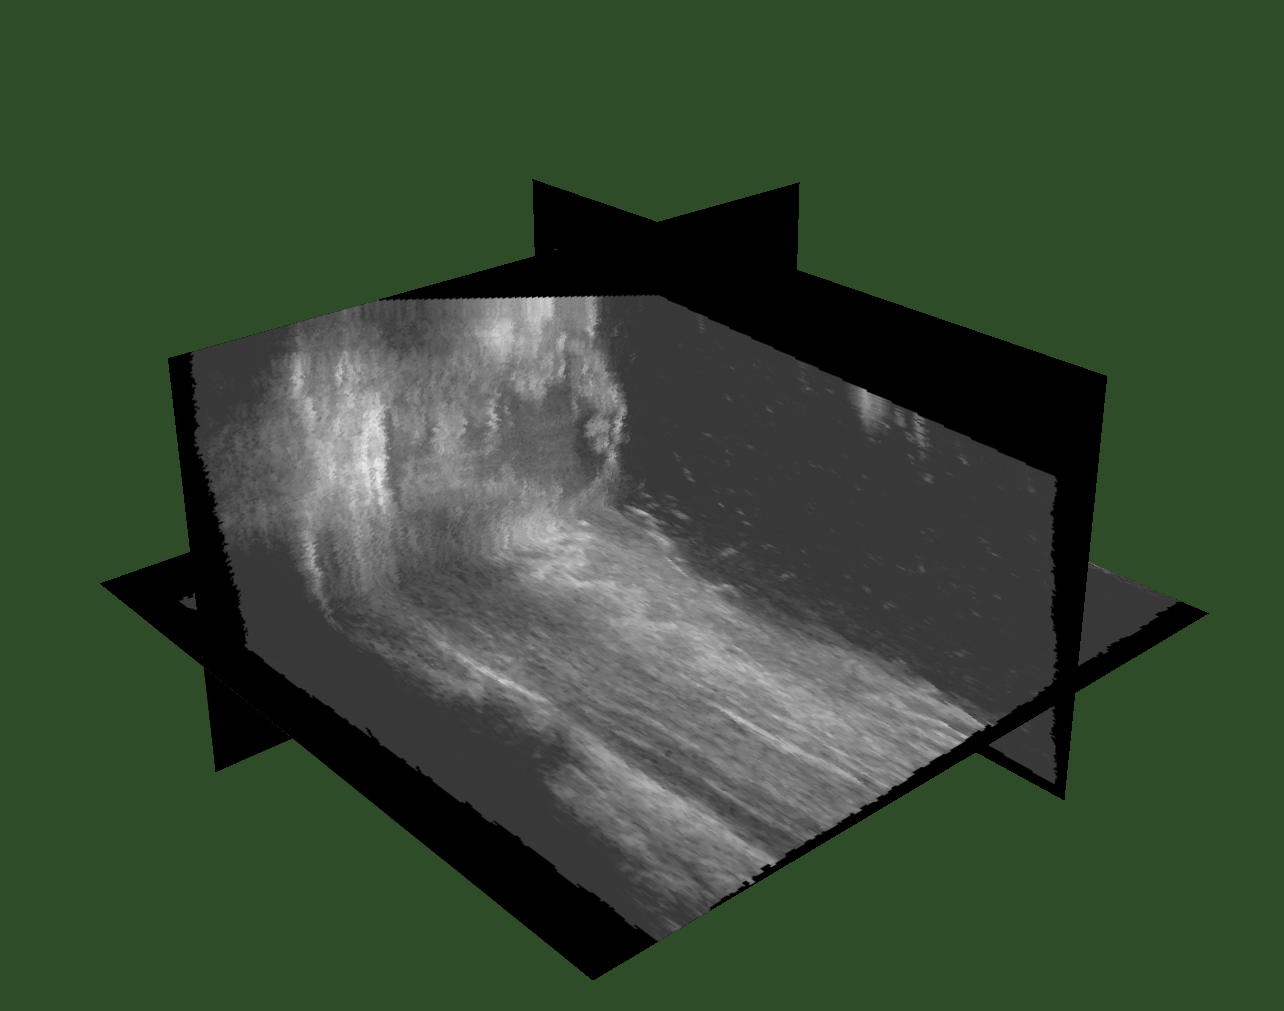
\includegraphics[width=0.49\textwidth]{graphics/orthogonal_screen1.png}
\caption[Screenshots of orthogonal MPR slices]{Screenshots of orthogonal MPR slices generated by our implementation}
\label{fig:orthogonal_screens}
\end{figure}

Figure \ref{fig:orthogonal_screens} shows some screenshots of the orthogonal MPR slices, and larger figures can be found in Appendix \ref{chapter:large_figures}. The slices are along each of the three volume axis, and the voxel values in each slice are rendered on the slice plane. This is performed by extracting voxel values on indices $(x,y,i)$, $(x,i,z)$ and $(i,y,z)$ for the z, y and x axis, respectively. The parameter $i$ determines where on each axis the slices are located, while $x$, $y$ and $z$ are all the possible voxel indices in the volume. The slices are extracted from the host memory volume and used as textures for three orthogonal polygons rendered with OpenGL. It should be noted that extracting the voxels and using them as textures takes a negligible amount of time. Using the mouse, the user can rotate the volume to view the slices at different angles, and pressing keyboard keys will increase or decrease the $i$ parameter. In this way, all parts of the volume can be visualized.

\subsection{Volume Ray Casting}
% pictchaz
% volume ray casted while on GPU
% one thread per ray
% build ray dirs kernel
% cast rays kernel
% do box-ray intersection to skip to volume before stepping
% set strength to max_voxel
% for each step:
	% if strength below cutoff -> end stepping
	% calculate transparency: min(1-voxel/max_voxel + adjustment, 1)
	% (if voxel below (other) cutoff -> set transparent to 1 (due to grey US background))
	% accumulate strength*(1-transparency)
	% update strength by multiplying with transparency
% set pixel to ray accumulation

\begin{figure}[h]
\centering
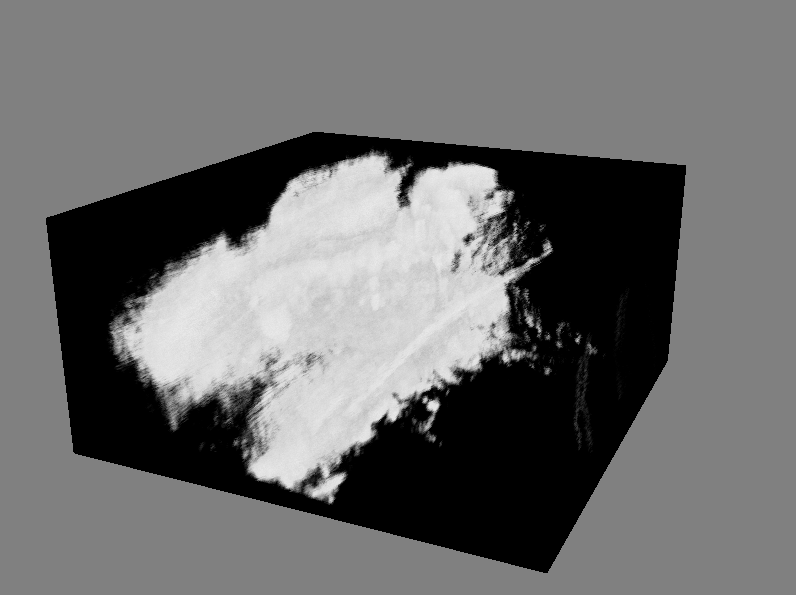
\includegraphics[width=0.49\textwidth]{graphics/raycast_screen0.png}
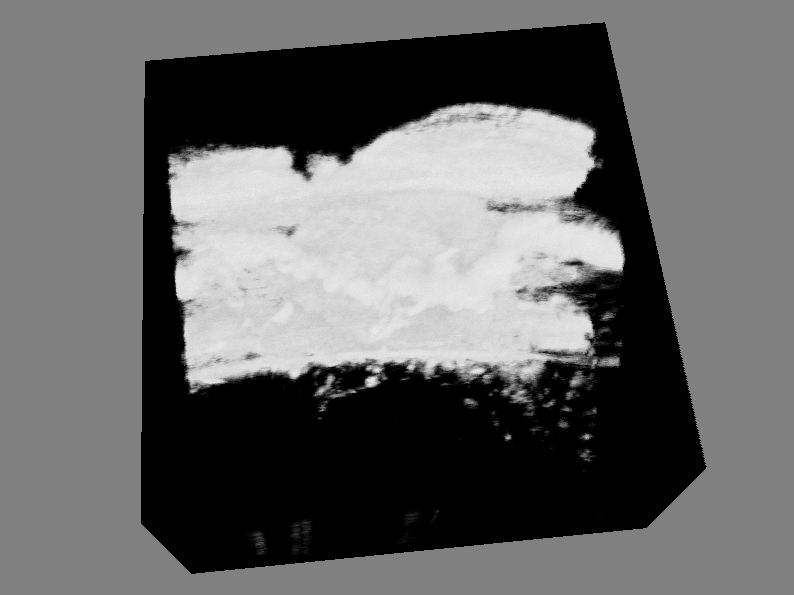
\includegraphics[width=0.49\textwidth]{graphics/raycast_screen1.png}
\caption[Screenshots of volume ray casting]{Screenshots of volume ray casting generated by our implementation}
\label{fig:raycast_screens}
\end{figure}

Figure \ref{fig:raycast_screens} shows some screenshots of the ray casted volume, and larger figures can be found in Appendix \ref{chapter:large_figures}. Ray casting is a computationally demanding task, but the GPU's processing power is utilized while the volume data is still on the device memory. The task is parallelized with one thread per ray, and consists of two steps: first construct the rays, then cast them into the volume.

Code listings of the implemented OpenCL kernels can be found in Appendix \ref{section:ray_casting_kernel}. The resulting rendered image consists of $w_s \times h_s$ pixels, with one ray (and thread) per pixel. The camera is defined by a camera location in space, a \emph{lookat} location that the camera is looking at, a vector defining "up" in the rendered image, and a vector defining "flat" (the horizontal direction) in the rendered image. Each ray's origin is the given camera location, but their direction needs to be calculated from their pixel position and a desired field-of-view. %This is done with Equation \ref{eq:ray_dir}.

%\begin{equation}
%	\label{eq:ray_dir}
%	r = \left| |camera_{lookat}-camera_{pos}| + FOV_{hor} camera_{right} \frac{x_{ray} - \frac{w_s}{2}}{\frac{w_s}{2}} + FOV_{vert} camera_{up} \frac{y_{ray} - \frac{h_s}{2}}{\frac{h_s}{2}} \right|
%\end{equation}

When the ray directions have been found, they can be cast into the volume. Instead of stepping from the ray origin, we save computations by first calculating the intersection between the box-shaped volume and each ray. This saves sampling for steps that are outside the volume.

There are many ways to accumulate voxel intensities while stepping along a ray. The method used in this work models the voxels as transparent cubes with a transparency level between 0.0 (fully oblique) and 1.0 (invisible). The entire procedure is as follows:

\begin{enumerate}
	\item $strength = 255$
	\item for each step along ray:
	\begin{enumerate}
		\item if $strength <$ cutoff, then break stepping
		\item $transparency = 1-\frac{intensity_{voxel}}{255}$
		\item accumulate $strength \cdot (1-transparency)$ into ray's pixel intensity
		\item $strength \leftarrow strength \cdot transparency$
	\end{enumerate}
\end{enumerate}

Each ray starts with a \emph{strength} parameter representing how much light has been absorbed. The initial value is the maximum value of a pixel (255), and it is reduced for each voxel encountered. For each voxel sampled, its intensity is weighted by the current strength and accumulated into the final pixel intensity. To save computations, the stepping is ended if the strength is below a given cutoff where the voxels simply do not contribute noticeable intensities.
	
\chapter{Analysis and Discussion of our Results}
	\label{chapter:results_discussion}
	
	% Repeat the motivation for the work
% Summarize what was done
% ? Explain why all goals have been met?

Ultrasound is a non-invasive, safe, low cost and practical way to provide medical doctors with an internal view of a patient's body. By performing 3D ultrasound reconstruction, 3D volumes can be constructed from 2D ultrasound scans, and be used for acquiring out-of-angle views, 3D rendering of the anatomy, and for image guided surgery. The purpose of this thesis was to investigate the parallel processing power of the GPU for fast ultrasound reconstruction. Having the ability to reconstruct a volume in a fraction of a second enables instant feedback and real-time incremental reconstruction while scanning. This thesis has presented our techniques to perform fast, non-incremental and real-time incremental reconstruction using the GPU. Optimization techniques for both pixel-based and voxel-based approaches have been described, and a novel method of doing real-time incremental reconstruction was presented. The performance obtained by these methods have been measured on some of the latest hardware architectures at the time of writing from both Nvidia and AMD. Issues for future work to look into are suggested in Section \ref{section:future_work}, and some final thoughts and closing statements are also given in Section \ref{section:final_thoughts}.
		
	\section{Performance}
	
		% intro
% outline

The goal of this thesis is to obtain real-time performance for 3D ultrasound reconstruction. Here, we present the measured performance of the methods described in the two previous chapters, and also identify how much of the computation time is spent on the different algorithmic steps on the device. We will first start by describing the test setup used in the measurements, then we present and discuss the performance obtained on different types of computing hardware (CPU and GPU). Last, the distribution of computation time between the different steps of the reconstruction procedure as well as the amount of memory required is presented and discussed.

% Test setup (hardware and input)
\subsection{Test Setup}

	Table \ref{table:test_computer} shows the hardware specifications of the computer used to measure the results in this chapter, with the different GPUs being used one at the time. All hardware is commercially available as commodity products.
	
	\begin{table}[h]
	\centering
	\begin{tabular}{| l l |}
		\hline
		$\bb{GPU}_1$ & Nvidia Tesla C2050 \\
		$\bb{GPU}_2$ & AMD ATI Radeon HD5870 \\
		$\bb{GPU}_3$ & Nvidia Quadro FX5800 \\
		\textbf{CPU} & Intel Core 2 Quad Q9550 \\
		\textbf{Memory} & 4 x 2 GB DDR3 \\
		\textbf{OS} & Microsoft Windows XP 64 bit \\
		\textbf{Compiler} & Microsoft Visual Studio 9.0 \\
		\hline
	\end{tabular}
	\caption[Test computer specifications]{Test computer specifications. See Table \ref{table:c2050hd5870} for GPU details}
	\label{table:test_computer}
	\end{table}
	
	Table \ref{table:test_input} gives a specification of the test input and volume size that was used for the performance tests. In parentheses are the symbols that from now on will be used to refer to these values. The tracking data were obtained from a Polaris optical tracking system (Northern Digital, Waterloo, Canada), and the b-scans from a Vivid 7 ultrasound scanner (GE Vingmed Ultrasound, Horten, Norway), equipped with a GE M12L linear array probe (GE Healthcare, Waukesha, WI).
	
	\begin{table}[h]
	\centering
	\begin{tabular}{| l l |}
		\hline
		\textbf{Number of b-scans ($n$)} & 434 \\
		\textbf{Number of tracking data} & 520 \\
		\textbf{B-scan size ($w \times h$)} & 768 x 576 pixels \\
		\textbf{Region-of-interest size ($m$)} & 342 x 356 pixels \\
		\textbf{Volume size ($w_{volume} \times h_{volume} \times n_{volume}$)} & 512 x 256 x 512 voxels \\
		\textbf{Pixel spacing x-dimension ($\Delta x$)} & 0.107724 mm \\
		\textbf{Pixel spacing y-dimension} ($\Delta y$) & 0.111732 mm \\
		\textbf{Voxel spacing all dimensions ($\Delta v$)} & 0.08 mm \\
		\textbf{Bits per pixel/voxel} & 8 \\
		\hline
	\end{tabular}
	\caption{Test input data}
	\label{table:test_input}
	\end{table}
	
	Most reconstruction algorithms have one or more parameters that increase the reconstruction quality at the cost of increased computational complexity. In Table \ref{table:test_parameters} a list of important parameter settings is provided for the algorithms that were considered.
	
	\begin{table}[h]
	\centering
	\begin{tabular}{| l l |}
		\hline
		\textbf{PNN} & $5^3$ neighbor voxels used for hole filling \\
		\textbf{VNN} & $5\Delta v$ distance cutoff to b-scans \\
		\textbf{Incremental PNN} & no hole filling \\
		\textbf{Incremental} $\bb{DWOP}_4$ & 4 b-scans interpolated per voxel \\
		\textbf{Incremental} $\bb{DWOP}_8$ & 8 b-scans interpolated per voxel \\
		\textbf{Incremental PT} & cubic interpolation of 4 b-scans per voxel \\
		\textbf{Ray casting} & 800 x 600 pixels (i.e. rays) \\
		\hline
	\end{tabular}
	\caption{Test algorithm parameters}
	\label{table:test_parameters}
	\end{table}

% present performance and speedup, and discuss speedup of GPU vs CPU for various algorithms (incl ray casting)
\subsection{GPU Performance}

	\begin{figure}[h]
	\centering
	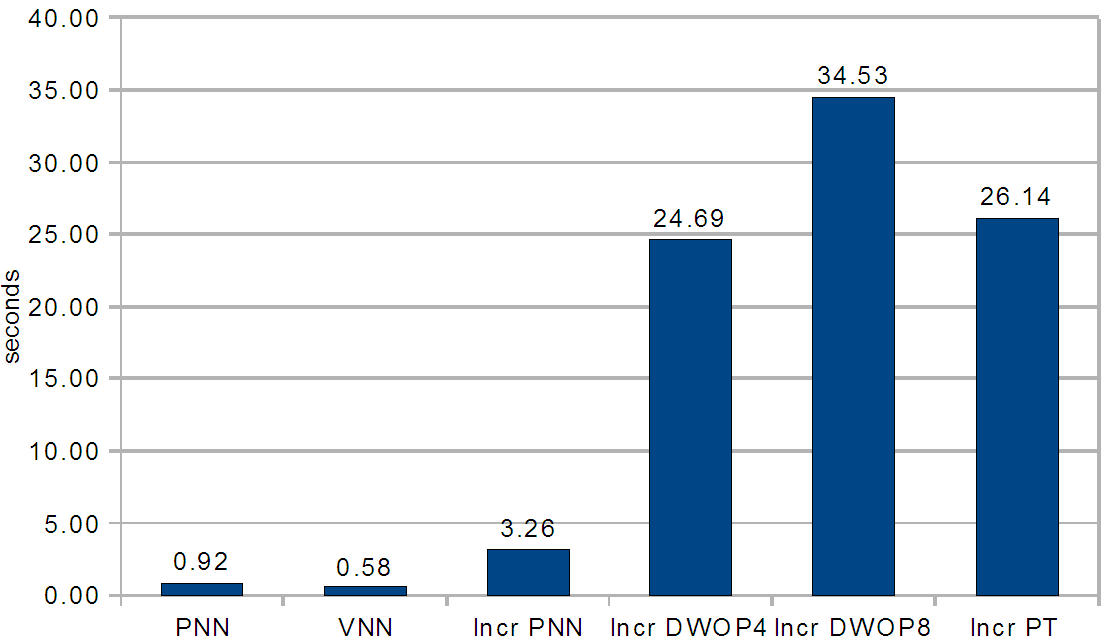
\includegraphics[width=\textwidth]{charts/gpu_performance.png}
	\caption{Reconstruction times using Nvidia Tesla C2050}
	\label{fig:gpu_performance}
	\end{figure}
	
	Figure \ref{fig:gpu_performance} shows the time measured when reconstructing the test input using the Nvidia Tesla C2050 for various algorithms. PNN and VNN are the non-incremental methods, and as one can see, they complete in under one second. The incremental PNN is slower, even without the hole filling, with the reason for this being the overhead associated with incremental reconstruction as previously described. The other incremental methods are substantially slower, and this is due to increased computations resulting in much higher reconstruction quality than the simple PNN. The incremental performance is, however, \emph{real-time} as about 20-30 seconds are typically used for freehand scanning.
	%Note how the incremental reconstruction method in this thesis is substantially better than simply performing a full PNN or VNN for each incoming b-scan. In that case, the reconstruction time would be roughly $434 \times 0.92 = 400$ and $434 \times 0.58 = 252$ seconds, respectively.
	
	The volume size is purposely set at the upper end of what one requires for normal use. Typically, the voxel spacing is set to the same value as the pixel spacing, so given a pixel spacing at around 0.1 mm the volume size would be $450 \times 200 \times 450$ voxels, which is 40 \% less than the one used for testing. The point to note is that these test sizes are \emph{worst case}.
	
	There are two variants of the distance weighted orthogonal projections (DWOP) method examined, which take into account 4 and 8 of the closest b-scans respectively. As can be seen, the increased quality obtained increases the reconstruction time by approximately 40 \%. The $DWOP_4$ and the method based on the probe trajectory (PT) take roughly the same time which can be explained by the fact that they both take 4 b-scans into account for each voxel evaluation. The PT method, however, is somewhat slower, which is explained by the higher degree of interpolation used. The complexity of the PT method is reflected by more complex code, which results in generally higher register use compared to the DWOP (49 \textit{vs.}\ 33 registers).
	
	\begin{figure}[h]
	\centering
	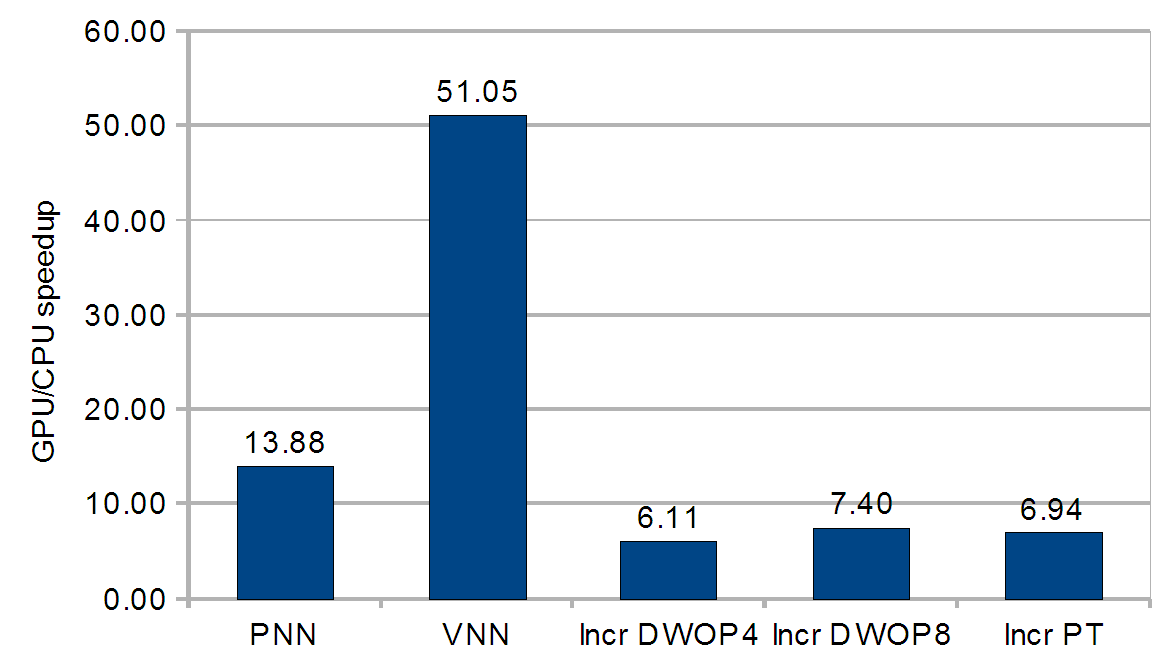
\includegraphics[width=\textwidth]{charts/gpu_cpu_speedup.png}
	\caption{Speedup of Intel Q9550 vs Nvidia Tesla C2050}
	\label{fig:gpu_cpu_speedup}
	\end{figure}
	
	The reconstruction methods were also implemented using only a single-threaded sequential CPU for the computations. In all cases the CPU was slower than the GPU version. Figure \ref{fig:gpu_cpu_speedup} shows the speedup of utilizing the GPU compared to only the CPU, with the performance of the GPU versions between 6 and 14 times faster, and 51 times faster in the case of VNN. In all cases, this is a substantial speedup. The main limiting factor in the speedup of the incremental cases is in the transfer of the volume at each increment (the specifics will be discussed in Section \ref{section:time_distribution}). One can see that the speedups of DWOP and PT are in the same order as their respective computation times. The explanation behind this is that increased computational load means that the processing power of the GPU can be utilized even more, and that the host-device transfers are smaller in comparison to the computations.
	
	While the non-incremental PNN gains a 14 times speedup, the non-incremental VNN gains a significant 51 times increase in performance. Note that these two algorithms are inherently different, and that they therefore cannot be expected to behave similarly to each other when utilizing the massively parallel GPU. One reason is the determinism of the implementations. Each of the threads in VNN reconstruction does exactly the same work, with a small difference at the end of the computations (based on  the voxel being in the ROI or not). For PNN this difference occurs early, as the pixels are processed in the beginning. Such branching results in low occupancy on the GPU, and makes it difficult to achieve good performance. As explained in Section \ref{section:non-incremental_pnn}, one of the major steps of the PNN algorithm is partitioned among "only" 434 threads, one per b-scan. While the VNN can use $w_{volume} \times h_{volume} \times n_{volume} = 512 \times 256 \times 512$ threads, i.e. one per voxel, which is a scalability more suitable to the massively parallel GPU. Furthermore, the hole-filling needed in PNN is a task similar in complexity to the VNN, and thus PNN in total should be slower than VNN. For more details on the difference between VNN and PNN performance, see Section \ref{section:time_distribution}.
	
	%\begin{table}[h]
	%\centering
	%\begin{tabular}{| l l |}
	%	\hline
	%	\textbf{Time for 100 renders} & \textbf{Renders/second (fps)} \\
	%	\hline
	%	\hline
	%	2.81 seconds & 35.6 \\
	%	\hline
	%\end{tabular}
	%\caption{Ray casting performance using Nvidia Tesla C2050}
	%\label{table:raycasting_performance}
	%\end{table}
	
	When using the Nvidia Tesla C2050, \textbf{100 renders} of the $512 \times 256 \times 512$ volume were ray casted in \textbf{2.81 seconds}, which is equivalent to \textbf{35.6 frames per second}. There are many definitions of how many frames per seconds are required to be considered \emph{real-time}, but a lower limit of 25 (PAL television format) or 30 (NTSC television format) should be sufficient. Given a lower limit of 1 update per reconstruction increment, 434 b-scans over 20 seconds would require a frame rate of 21.7. Thus, the performance is more than sufficient for real-time display.

% explain speedup of Fermi vs Quadro and Radeon (and Mac?) for various algorithms
\subsection{Performance of GPU Platforms}

	\begin{figure}[h]
	\centering
	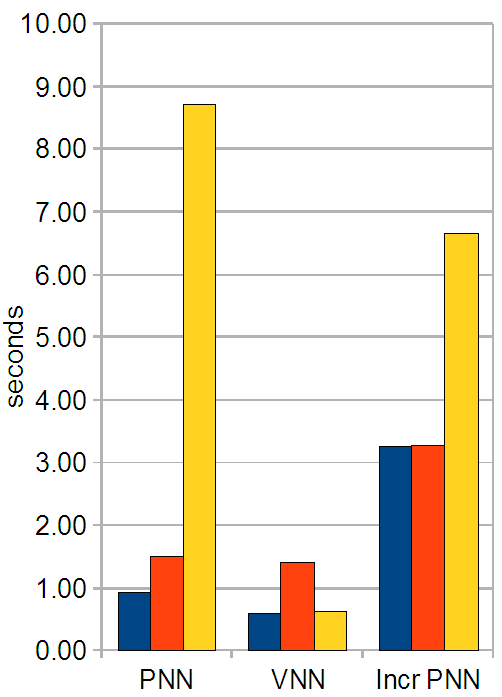
\includegraphics[height=0.33\textheight]{charts/platforms_performance_1.png}
	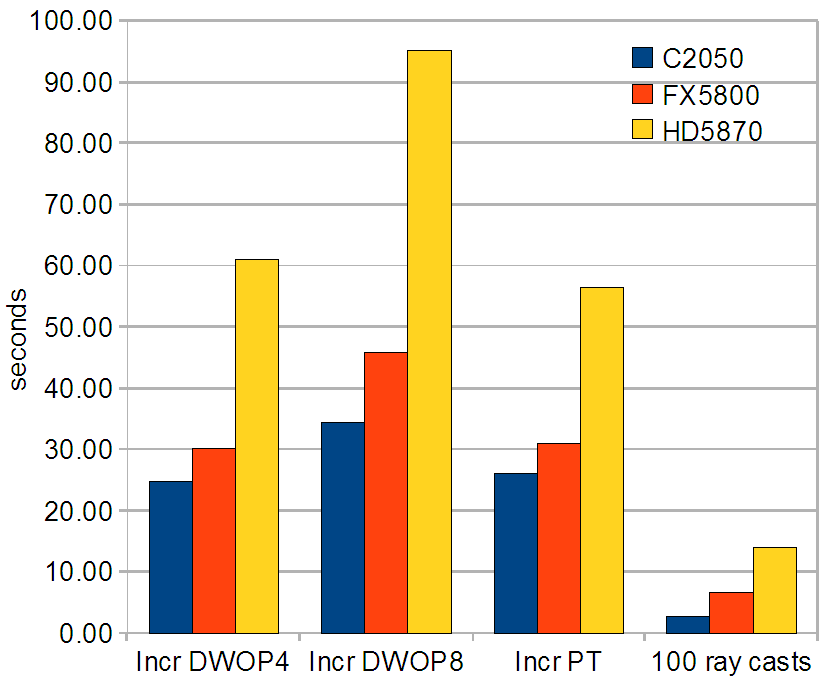
\includegraphics[height=0.33\textheight]{charts/platforms_performance_2.png}
	\caption[Performance of reconstruction and ray casting]{Performance of reconstruction and ray casting on Nvidia Tesla C2050, AMD HD5870 and Nvidia Quadro FX5800}
	\label{fig:platforms_performance}
	\end{figure}
	
	It should now be established that reconstruction performance is substantially greater using the GPU. However, several GPU platforms are available for comparison. The C2050 is at the time of writing the latest and most powerful generation on the market. By using the multiplatform OpenCL standard \cite{openclspec}, it is possible to execute the code on both Nvidia and AMD GPUs. Figure \ref{fig:platforms_performance} shows the performance obtained on the C2050, the older FX5800 also from Nvidia, and the HD5870 from AMD. In terms of prior expectations, the FX5800 is one of the most powerful of the \emph{previous} generation of Nvidia GPUs, and the HD5870 is expected to place itself roughly halfway between these two cards.
	
	With these presumptions, the performance results both confirm and surprise. The C2050 performs better than the FX5800 in all cases, with up to 2.5 times the performance. While in some cases (like incremental PNN) the performance is almost equal or only slightly better, but this will be explained below. The HD5870 however, disappoints in all except in the one case of VNN, with performance typically around 50 \% of the FX5800 and as low as 17 \% in the case of PNN. Just as VNN proved to be very suitable for the GPU with a speedup of 51, it also seems to be the case on the HD5870 and compares favorably with a performance close to the much newer C2050. In the other cases, it can be pointed out that the OpenCL standard was made with CUDA in mind because of its status as a \emph{de facto} standard at the time. AMD's OpenCL implementation obviously has room for improvement, and the potential is clearly there as seen with the performance of VNN. It should be noted however, that in all the cases the HD5870 is still between 1.5 and 3.2 times faster than the pure CPU implementation (and 47 times faster for VNN).
	
	As mentioned, the C2050 beats the older FX5800 in all the cases, but one notices that the gap is substantially narrower for the incremental methods. The explanation in these cases is due to the time spent on transferring the volume. Even though C2050 represents the next generation of Nvidia GPUs, the data bus between host and device (PCI Express) is identical for both. This is evident in the cases of incremental reconstruction, where the computations are lighter for each increment. Again, this is confirmed by a greater relative gap (1.23 \textit{vs.}\ 1.33) between $DWOP_4$ and $DWOP_8$, where the only difference is computational complexity.
	
	In the case of VNN and ray casting, the C2050 offers 2.5 and 2.4 times the performance of the FX5800, but the C2050 has only about twice the number of computational cores of the FX5800 and 40 \% increased memory bandwidth \cite{c2050, fx5800}. The explanation is one key feature to the Fermi GPU architecture which C2050 belongs to, the addition of L1 and L2 cache. With a L1 cache per streaming multiprocessor and a global L2 cache for all computation cores, the effective memory bandwidth can be drastically increased depending on the application. If the same data is read repeatedly by several threads, the values will be available in this fast cache. This is especially the case for VNN, where the b-scan plane equations and corner points are read repeatedly by neighboring threads, and also for ray casting where neighboring rays read the same voxel data. In both cases it is hard to estimate exactly which groups of threads will require what groups of common data, but the cache handles this temporal locality automatically.

% which steps of algorithms take how long computation time w/ explanation
	% steps on GPU (i.e kernels)
	% CPU steps (interpolation, calibration, setting up data structures, etc)
\subsection{Distribution of Reconstruction Time}
	\label{section:time_distribution}
	
	To gain a deeper understanding of the reconstruction performance for each method, one has to look at the time is takes to do the various reconstruction steps and the data transfers between device and host. In this section we present this distribution, and explain why it occurs like it does. In all cases, the C2050 has been used for the measurements. 
	
	\begin{figure}[h]
	\centering
	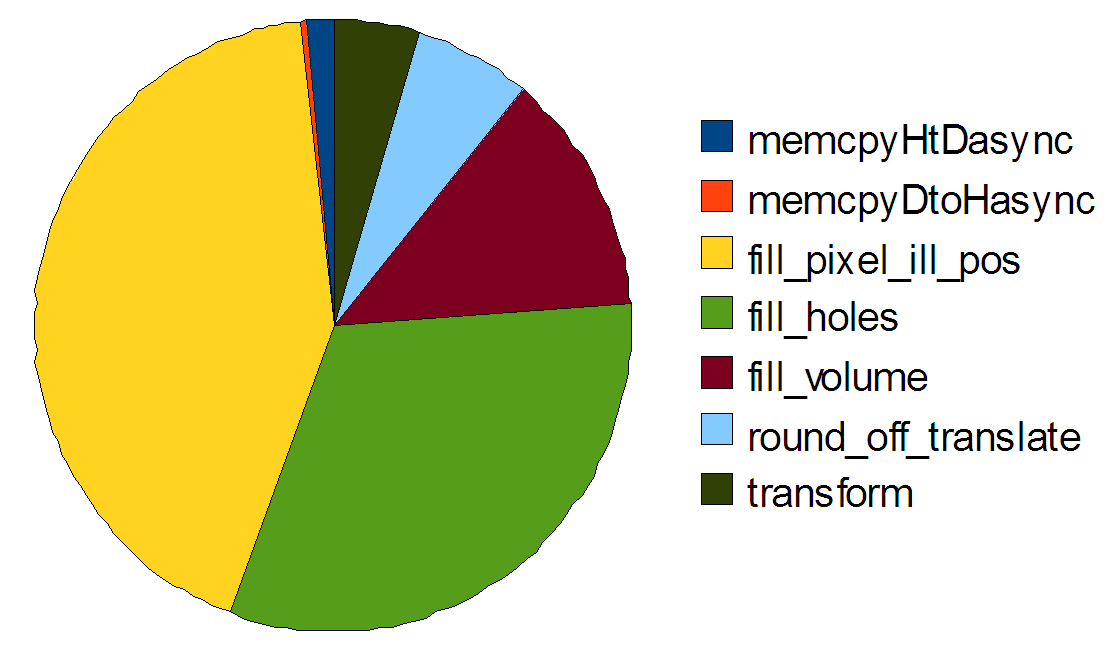
\includegraphics[height=0.3\textheight]{charts/pnn.png}
	\caption[Distribution of computation time for PNN]{Distribution of computation time on Nvidia Tesla C2050 for PNN}
	\label{fig:pnn_pie}
	\end{figure}
	
	Figure \ref{fig:pnn_pie} shows the distribution of the time for PNN on the GPU. Note that transfers between host and device (memcpyHtoDasync and memcpyDtoHasync) are negligible compared to the computations. In this case, around 200 MB (mainly from b-scans) is transferred to the device and 67 MB (the volume) is transferred back. The GPU is connected to the host via a PCI Express 2.x 16X bus, which has an upper transfer limit of 8 GB/s. These small data sizes are thus negligible. The largest portion is the task of filling $pixelill$ and $pixelpos$, and as previously discussed, this is hard to parallelize, and is indicated by a GPU core occupancy of only 17 \% during this step. The rest of the steps all have a 100 \% occupancy. However, there are two other tasks that also take up a large part of the time: filling the volume and (especially) filling the holes. Actually, processing all the ROI-pixels and inserting them into the volume actually takes less time than filling those holes. This demonstrates how the PNN performance is penalized by the hole filling required due to of the nature of the algorithm.
	
	\begin{figure}[h]
	\centering
	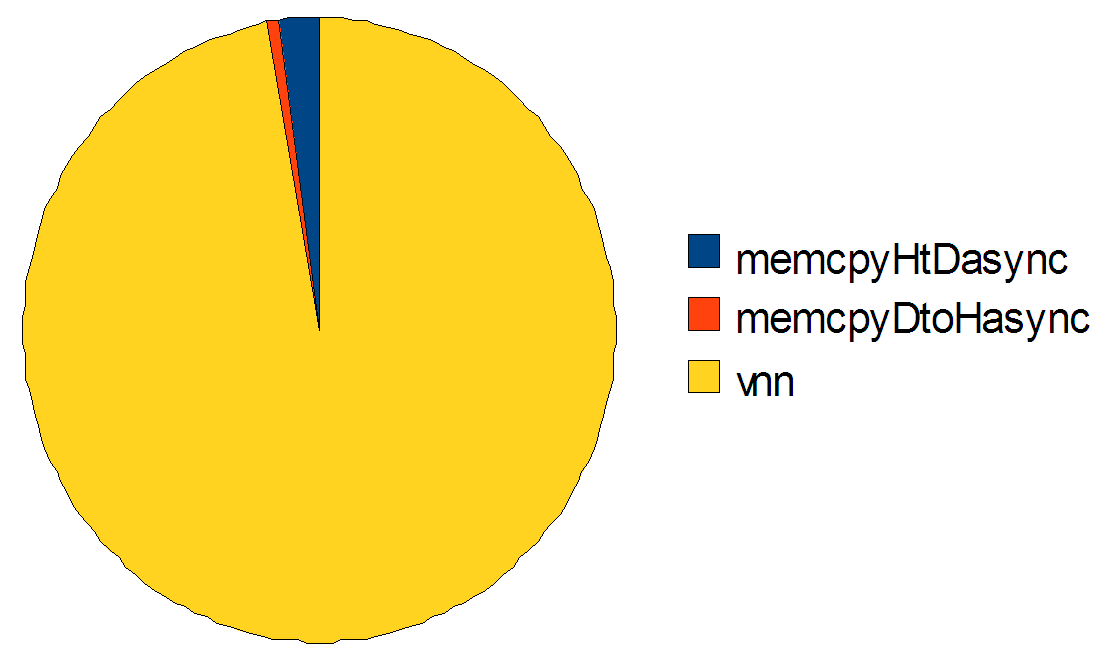
\includegraphics[height=0.3\textheight]{charts/vnn.png}
	\caption[Distribution of computation time for VNN]{Distribution of computation time on Nvidia Tesla C2050 for VNN}
	\label{fig:vnn_pie}
	\end{figure}
	
	Figure \ref{fig:vnn_pie} shows the distribution of time for VNN on the GPU. As in the case with PNN, the transfers between host and device are negligible (in fact, they are of the same absolute sizes as in PNN). Unfortunately, the VNN reconstruction was implemented as a single GPU kernel, and thus the distribution between steps cannot be identified.
	
	\begin{figure}[h]
	\centering
	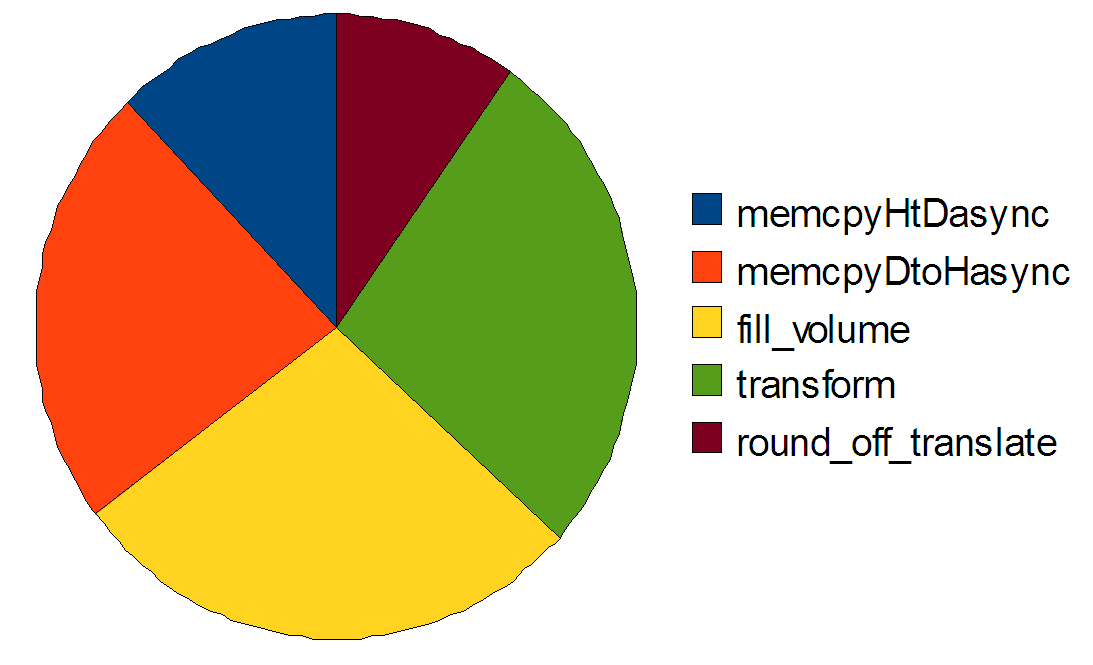
\includegraphics[height=0.3\textheight]{charts/incr_pnn.png}
	\caption[Distribution of computation time for incremental PNN]{Distribution of computation time on Nvidia Tesla C2050 for incremental PNN}
	\label{fig:incr_pnn_pie}
	\end{figure}
	
	Figure \ref{fig:incr_pnn_pie} shows the distribution of time for incremental PNN on the GPU. As opposed to the non-incremental cases, transfers between host and device take a noticeable share as more than a third of the time is now consumed on this. For each increment, a tracking matrix and the $pixelpos$ and $pixelill$ for one b-scan must be transferred, approximately 1.6 MB. The transfer back of the transformed $pixelpos$ is approximately 1.4 MB. However, the overhead associated with each transfer adds up, as demonstrated by the large share of the total time. This overhead is especially noticeable for incremental PNN, due to the total time spent per increment being relatively smaller.
	
	\begin{figure}[h]
	\centering
	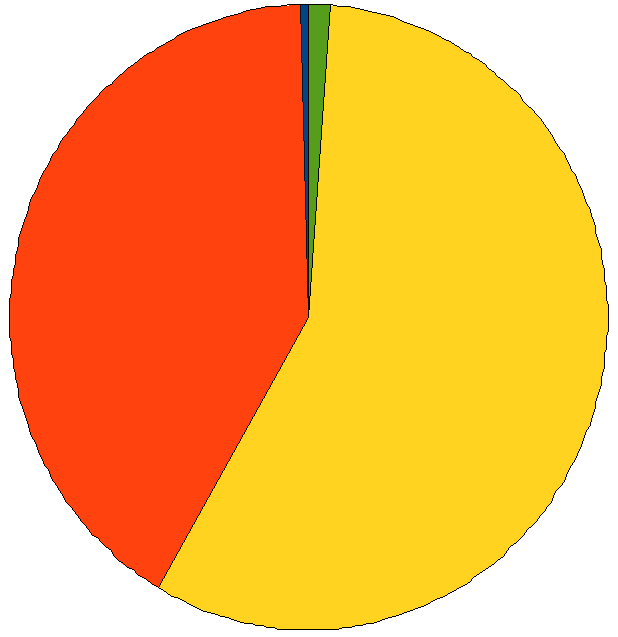
\includegraphics[height=0.175\textheight]{charts/incr_hq_1.png}
	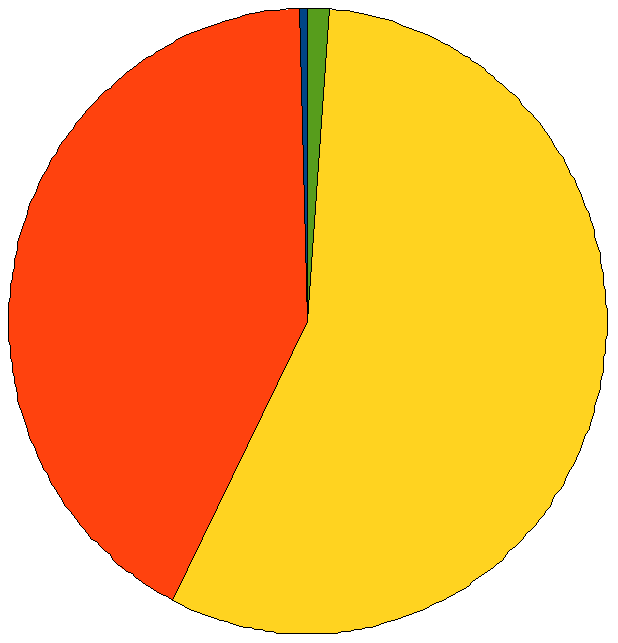
\includegraphics[height=0.175\textheight]{charts/incr_hq_2.png}
	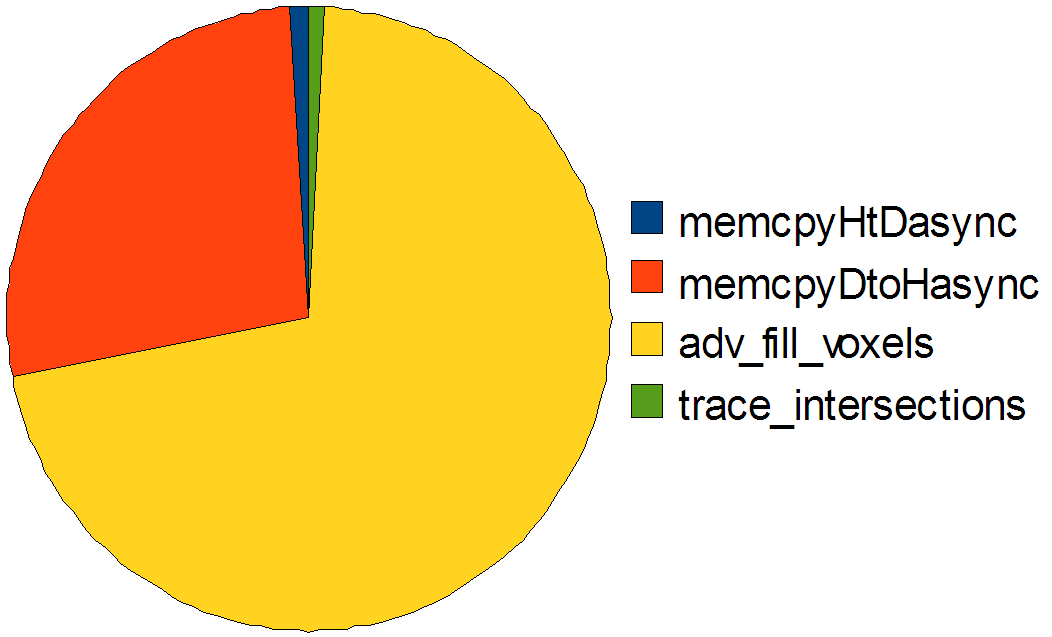
\includegraphics[height=0.175\textheight]{charts/incr_hq_3.png}
	\caption[Distribution of computation time for PT, $DWOP_4$ and $DWOP_8$]{Distribution of computation time on Nvidia Tesla C2050 for PT, $DWOP_4$ and $DWOP_8$}
	\label{fig:incr_hq_pie}
	\end{figure}
	
	The other incremental methods share the same characteristics in the time distribution, as shown in Figure \ref{fig:incr_hq_pie}. The transfers between device and host take up a big share, but this is only \emph{from} the device \emph{to} the host, as host to device is practically negligible. The reason for this is that as each increment takes a substantially longer time in these methods than in incremental PNN, and the overhead of the small host-to-device transfer is hidden, while transferring the 67 MB volume for each increment still takes its share of the total time. The same reasoning explains why $DWOP_8$ has a smaller share of transfers than $DWOP_4$; i.e.\ each increment is more computationally complex. In fact, incremental PT and $DWOP_4$ has almost identical time distributions, which is not surprising as their computational complexity is very similar. As can be seen in the charts, the task of finding the voxels between two b-scans (trace\_intersections) is negligible, rather is the filling of those voxels by PT or DWOP that take up all the computation time.
	
	\begin{figure}[h]
	\centering
	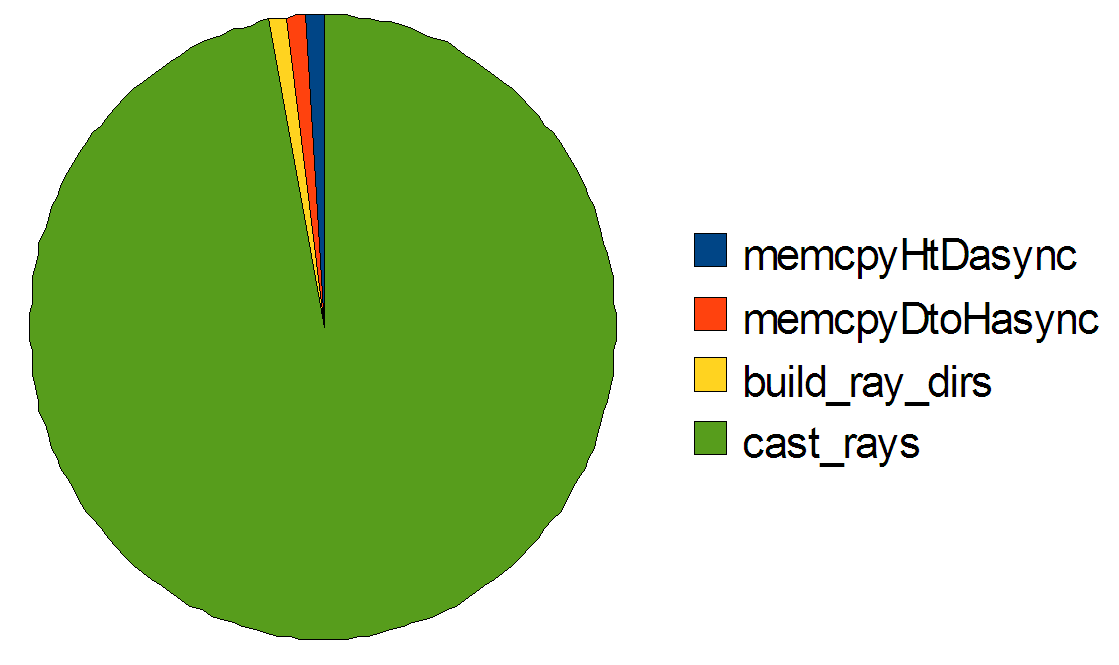
\includegraphics[height=0.3\textheight]{charts/ray_casting.png}
	\caption[Distribution of computation time for ray casting]{Distribution of computation time on Nvidia Tesla C2050 for ray casting}
	\label{fig:ray_casting_pie}
	\end{figure}
	
	Figure \ref{fig:ray_casting_pie} shows the distribution in the time for ray casting on the GPU. One quickly sees that transfers between host and device are negligible, as is expected given only a few camera parameters are sent to the device and a 480 KB rendered frame is sent back. This demonstrates the advantage of already having the reconstructing volume in the device memory, making additional transfers unnecessary. Building the ray directions is also a simple task, as demonstrated in the chart, and this is easily explained when one takes into account that the number of rays to be built is only $800 \times 600 = 480,000$, while the number of voxels to be sampled is $512 \times 256 \times 512 = 67,108,864$.
	
% present and discuss how much memory is used in all algs (make table with buffers and total)
\subsection{Memory Use}

	\begin{figure}[h]
	\centering
	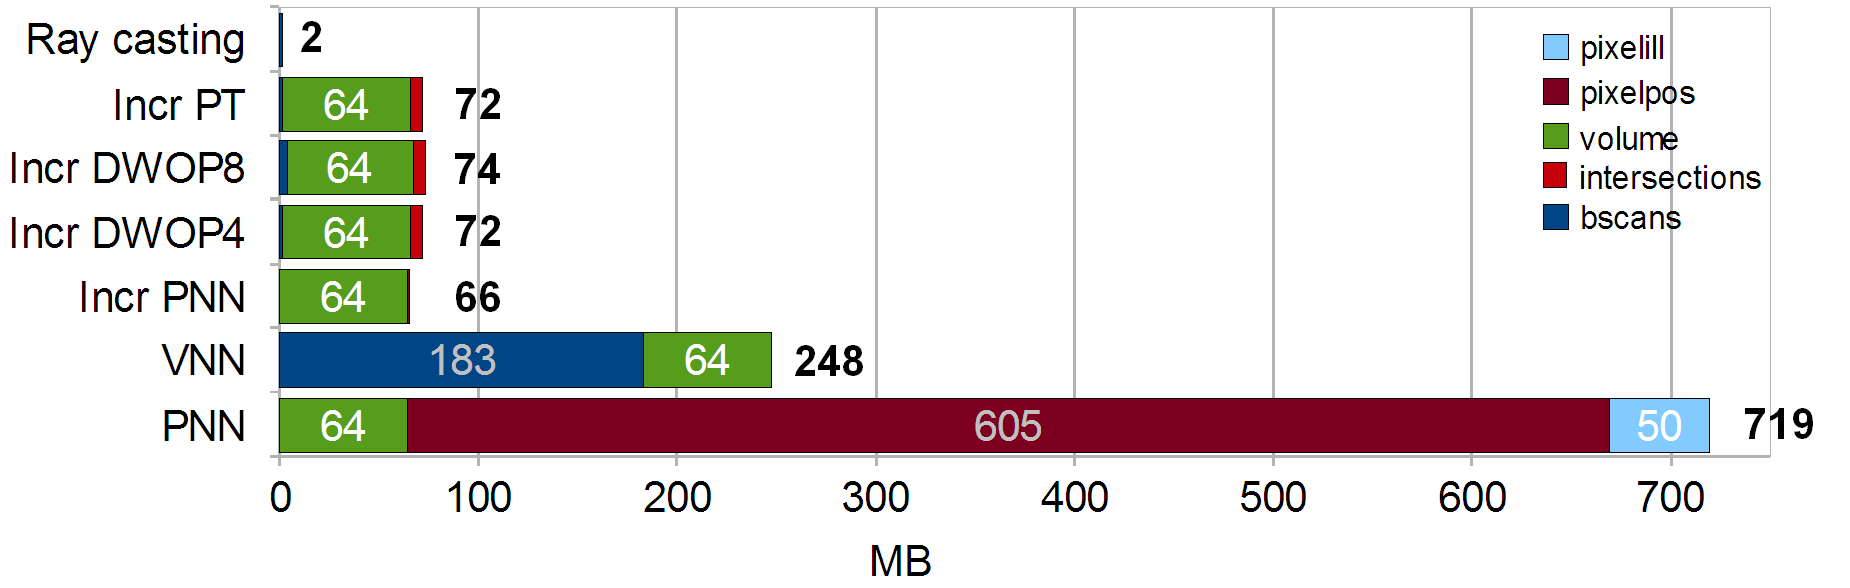
\includegraphics[width=\textwidth]{charts/memory_use.png}
	\caption{GPU memory use}
	\label{fig:memory_use}
	\end{figure}
	
	The chart in Figure \ref{fig:memory_use} shows how much GPU memory is used by each reconstruction method and the ray casting when using the previously described test data as input. It is easy to see that PNN uses the most memory, a total of 719 MB. Actually, it also requires 183 additional megabytes for the input b-scans, but as these are processed into the 50 MB $pixelill$ at the beginning of the procedure they can subsequently be freed from the GPU memory, hence they are not shown in the chart. The biggest contribution to PNN's memory usage is the $pixelpos$, and this is not surprising with three 4-byte coordinates required per pixel. The VNN on the other hand, requires only the input b-scans and output volume. In all cases, there are negligible amounts of memory used for tracking data, timetags, etc. These are so insignificant that they are not noticeable in the chart, and are so not of interest in this discussion.
	
	The incremental methods are quite similar in that they do not use much memory except for the volume, because the input is processed in small chunks at the time. While incremental PNN only keeps a single b-scan in memory at the time, incremental DWOP and PT utilize a "window" of b-scans and other data as previously described in Section \ref{section:incr_hq_impl}. $DWOP_4$ and PT have a window size of 4, resulting in approximately 1.7 MB for b-scans and other data, while $DWOP_8$ uses 8, requiring approximately 3.5 MB, all relatively small amounts of data. The ray casting of course needs a volume to render, but it is assumed that this is already present in the device memory, and so only an additional 2 MB is required (and most of it is the rendered frame).

% present and discuss how the algorithms scale with problem size (and processing capacity?)
	% voxel-based vs.\ pixel-based computational complexity (big-oh-ish)
	% computation complexity of incremental approach (big-oh-ish)
	% ? measure and make some scaling graphs of the most relevant parameters
%\subsection{Scaling}
		
	\section{Reconstruction Quality}
	
		% intro/motivation
% present test input (refer to performance section, but include some b-scans)
% present a reconstructed volume from all axis

The last section discussed the quantitative performance of the presented methods of this thesis. Obviously, there may be a reason for not simply choosing the fastest method above all else, and that reason is reconstruction quality. Thus, for a full evaluation both performance and reconstruction quality need to be taken into account. In this section, we discuss reconstruction quality and present the quality of the various methods. The effect of noise in the tracking data and choice of compounding method is also discussed. In Appendix \ref{chapter:large_figures}, large uncropped figures can be found.

The test input is the same as given in the performance results section. As a reference point, Figure \ref{fig:example_b-scans} shows some b-scans from this set. As seen in the b-scans, the probe used is of the linear type. The reconstructed volumes from each method will be presented shortly, but since they are in general very similar, we will extract an interesting part of the volume for each method. To get a view of what the volumes reconstructed by the methods described look like, Figure \ref{fig:example_volume} shows a typical reconstruction result (obtained using the PT method).

	\begin{figure}[h]
	\centering
	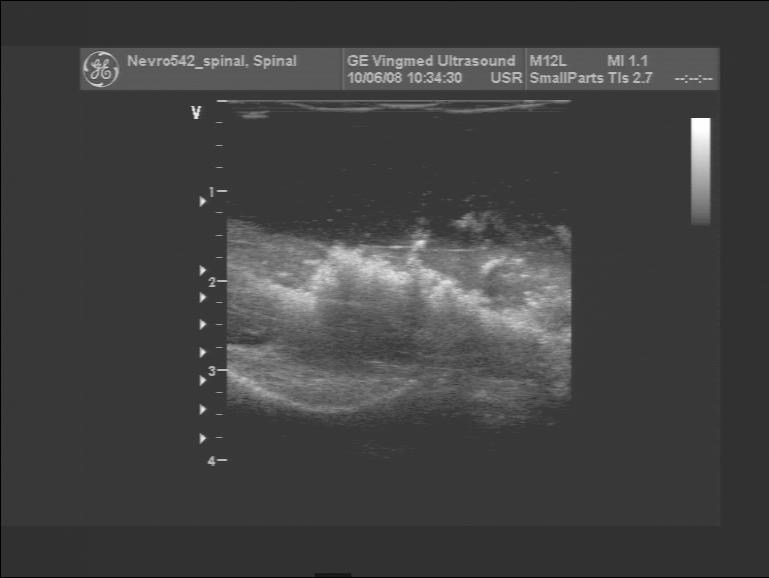
\includegraphics[width=0.49\textwidth]{graphics/60.png}
	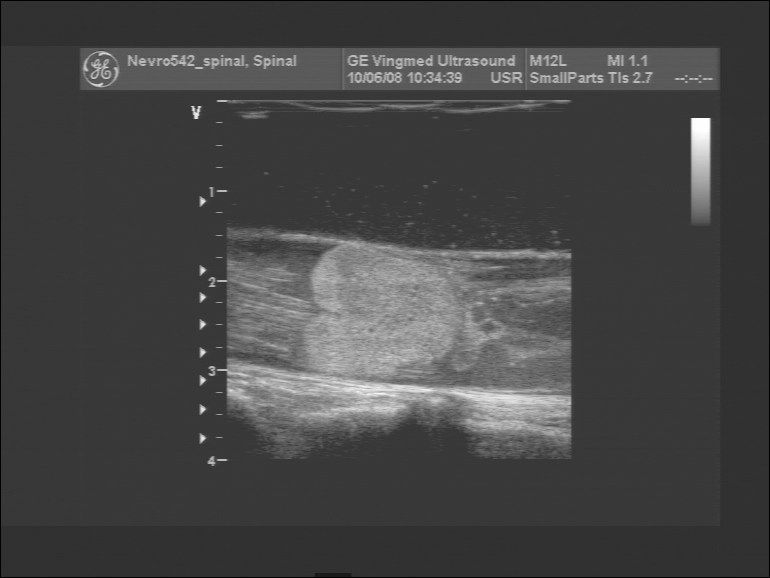
\includegraphics[width=0.49\textwidth]{graphics/280.png}
	\caption[B-scan examples from input set]{B-scan number 60 and 225 of the input set given in Table \ref{table:test_input}}
	\label{fig:example_b-scans}
	\end{figure}
	
	\begin{figure}[h]
	\centering
	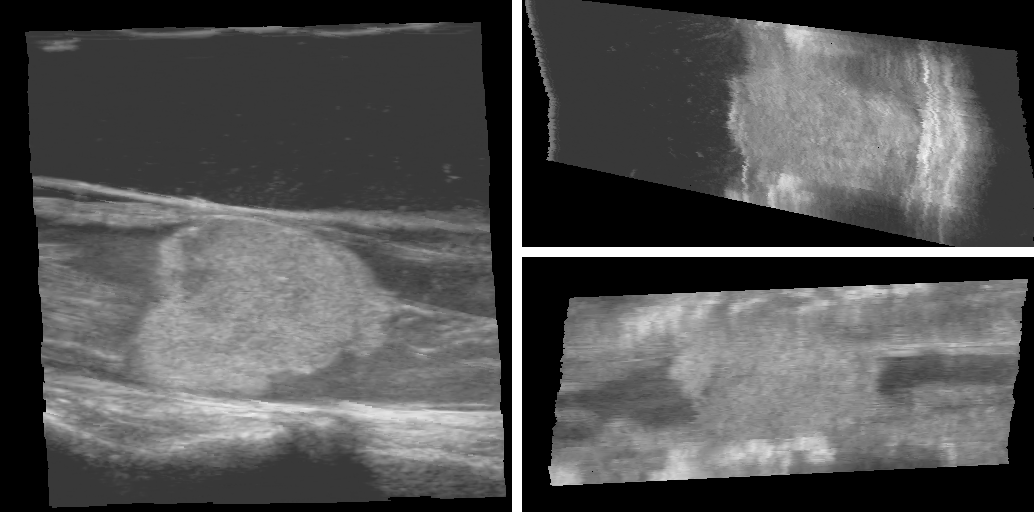
\includegraphics[width=\textwidth]{graphics/example_volume.png}
	\caption[Example volume]{Example of three orthogonal slices of a reconstructed volume (left: X-axis, top-right: Z-axis, bottom-right: Y-axis) generated by our implementation}
	\label{fig:example_volume}
	\end{figure}

% discuss what is meant by quality (close to ground truth, fact: input data less than output data, averaging blurs, tradeoff between hidden positives and false positives)
\subsection{What is Quality}

	It is difficult to define a scale for a qualitative measure such as reconstruction quality. The goal of reconstruction is to be as close to the ground truth as possible, but the reality is that given a ROI of $342 \times 356$ bytes over 434 b-scans and an output volume of $512 \times 256 \times 512$ bytes, the input is only 79 \% of the output. This means that in the case of our test data, even with a perfect reconstruction algorithm, the true volume cannot be calculated as some interpolation is required.
	
	So given that the volume will be an estimate, the discussion is what the \emph{best} estimate is, and this also depends on how the volume will be used. Ultrasound scans are analyzed by trained medical personnel, and one of the main uses of the reconstructed volume is to be examined by such people. There is an important tradeoff between avoiding false positives and hiding true positives. A false positive is an artifact of the data set that the analyzer can misinterpret as some symptom that in fact do not exist, while a hidden true positive is an actual existing artifact that is not noticeable by the analyzer. Both cases are unwanted. However, one can argue that the latter case is more important to avoid.
	
	%The various techniques for filling the missing data usually employ some sort of averaging or interpolation. Furthermore, unwanted noise in the input can be reduced by averaging redundant data. Such averaging has the advantage of reducing false positives due to noise or imperfect reconstruction schemes, but it can also hide true positives.

% discuss effect of noise in tracking data with lines.vol example
\subsection{Effect of Noise in Tracking Data}

	\begin{figure}[h]
	\centering
	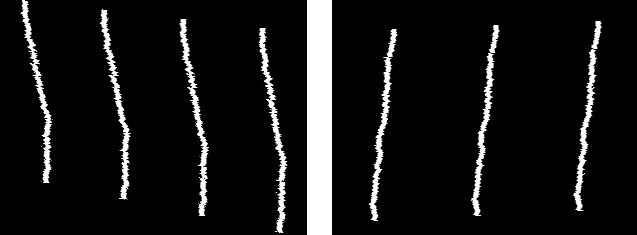
\includegraphics[width=\textwidth]{graphics/tracking_noise.png}
	\caption[Noise in the tracking data]{Noise in the tracking data seen in reconstructed volume (left: seen along Z-axis, right: seen along X-axis) generated by our implementation}
	\label{fig:tracking_noise}
	\end{figure}

	Any reconstruction method can only be as good as the input it is given. For the input data used in this thesis, the quality of the ultrasound b-scan images was more than adequate compared to the quality of the tracking data. For the test data used in this chapter, the ROI is $3.7 \times 4.0$ cm in world space, and the freehand movement covers a stretch of about 2 cm. When dealing with such small sizes, inaccuracies in the tracking can be expected. Figure \ref{fig:tracking_noise} shows the result of reconstructing images of straight lines using the tracking data. One can clearly see the oscillating disruption from the general probe trajectory. The effect is especially noticeable because of the small distances between adjacent scans.
	
	A plausible explanation could be that the freehand movement of the probe actually was jittery (e.g.\ an unsteady hand), but if one would look at the input b-scans before reconstruction, one would see that details are preserved on the same location over several neighbor images without any jitters. Thus, we conclude that the accuracy of the tracking data is poor, and this affects the results of all reconstruction methods.

% discuss reconstruction quality of the various algorithms
	% grid of screens (one axis, cropped on interesting part (same for all))
	% discussion of quality of each alg, w/ various zoomings of interesting stuff to illustrate
\subsection{Reconstruction Quality Results}
	
	Figure \ref{fig:crops} shows the results of various reconstruction methods. An interesting region of the volume is cropped from the rest to make it easier to spot key differences, and uncropped large figures can be found in Appendix \ref{chapter:large_figures}. Each crop is a slice of the same area looking in the direction of the X-axis. The compounding method used for all methods is $overwrite$.
	
	\begin{figure}[h]
	\centering
	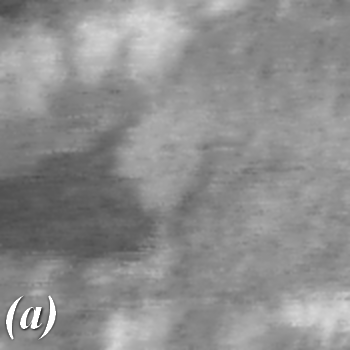
\includegraphics[width=0.48\textwidth]{graphics/crop_pnn.png}
	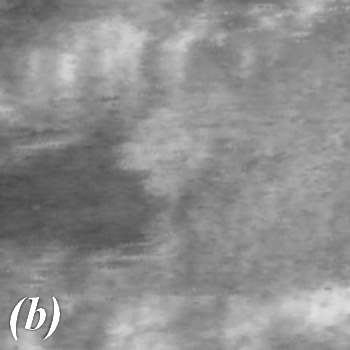
\includegraphics[width=0.48\textwidth]{graphics/crop_vnn.png}
	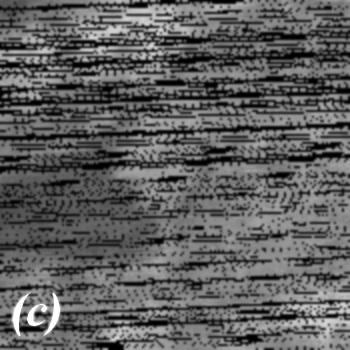
\includegraphics[width=0.48\textwidth]{graphics/crop_pnn_holes.png}
	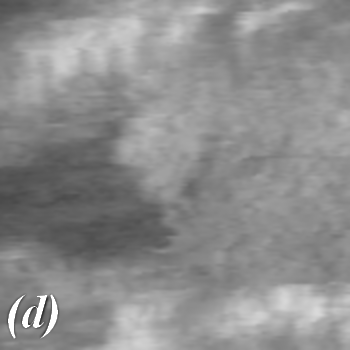
\includegraphics[width=0.48\textwidth]{graphics/crop_dwop4.png}
	\includegraphics[width=0.48\textwidth]{graphics/crop_dwop8.png}
	\includegraphics[width=0.48\textwidth]{graphics/crop_pt.png}
	\caption[Cropped section of reconstructed volume]{\small Cropped section of reconstructed volume generated by our implementation. \textbf{$(a)$} PNN. \textbf{$(b)$} VNN. \textbf{$(c)$} PNN w/ no hole filling. \textbf{$(d)$} incremental $DWOP_4$. \textbf{$(e)$} incremental $DWOP_8$. \textbf{$(f)$} incremental PT.}
	\label{fig:crops}
	\end{figure}
	
	\clearpage
	
	\subsubsection{PNN Quality} % also Incr PNN (PNN no hole filling)
	
		As seen in Figure \ref{fig:crops}a, the PNN is somewhat grainy, and this is expected when using only the nearest neighbor for filling instead of some method of weighting. Some of the grains are also due to the fact that there are not enough pixels to fill the entire volume. This means that along a row of pixels, at some point a voxel is skipped. E.g.\ if there are 20 pixels along a row of a b-scan, and they are reconstructed onto a voxel that has 25 voxels along a row of the same size, then 5 voxels are periodically left empty. This is clearly seen in Figure \ref{fig:crops}c where hole filling is turned off. In addition to the black lines of holes between b-scans, there are periodical holes every 4-5 voxels in a grid because the pixel spacing is $\simeq 0.1$, while the voxel spacing is $0.08$, i.e.\ $\frac{0.1}{0.08} = 1 \frac{1}{4}$. Additionally, one can also see the tendency for horizontal lines in the image, but this is mainly due to the tracking noise discussed earlier, and is present in all cases.
	
	\subsubsection{VNN Quality}
	
		One can see in Figure \ref{fig:crops}b that the VNN is sharper than the PNN. More details are preserved in the white spots at the top, and the texture of the gray area at the right is more clearly visible. This can be caused by the smoothing effect of averaging voxels when filling the PNN holes. The VNN method is still based on nearest-neighbor however, and also suffers from graining as the PNN method. This is unavoidable as two neighboring voxels often have different closest b-scans when the scans are packed together.
	
	\subsubsection{Incremental DWOP Quality} % DWOP4 and DWOP8
	
		$DWOP_4$ and $DWOP_8$, shown in Figure \ref{fig:crops}d and \ref{fig:crops}e, do not have the problem of grains that occurs with PNN and VNN. This is of course because several b-scans influence each voxel, and those b-scans are weighted differently. The drawback, however, is a slightly noticeable blurring of the volume when compared to VNN. However, one can argue that the sharper features of VNN might be largely due to the effect of the grains, thereby effectively allowing a cluster of grains to be mistaken as a feature.
		
		The difference between $DWOP_4$ and $DWOP_8$ is not substantial, but the $DWOP_8$ is slightly smoother than the $DWOP_4$. This is explained by the fact that $DWOP_8$ weights \emph{eight} neighbor b-scans instead of \emph{four}, and thus each voxel is influenced by b-scans further away than with $DWOP_4$, causing the blurring. Since the weighting is distance based, this blur is minor, but the similarity between $DWOP_4$ and $DWOP_8$ does not justify the increase in computation time associated with $DWOP_8$.
	
	\subsubsection{Incremental PT Quality}
	
		The result of the PT method is shown in Figure \ref{fig:crops}f, and as the other weighting based methods, it does not contain grains. However, in comparison to DWOP, it is clearer and sharper, with the details of the white area at the top and the texture of the gray area to the right being superior to those from other methods. With PT having only a slightly greater computation time than $DWOP_4$ it is evident from this thesis that PT is a superior method.		
		
		To illustrate another advantage of the PT method, Figure \ref{fig:sparse} and shows the results when the input is sparse. With more space between the b-scans, the approach to filling this space becomes more important. Figure \ref{fig:sparse_lines} highlights the differences even more by using straight lines instead of ultrasound b-scans (but using the real tracking data).
		
		\begin{figure}[h]
			\centering
			\includegraphics[height=0.2\textheight]{graphics/dwop8_sparse.png}
			\includegraphics[height=0.2\textheight]{graphics/pt_sparse.png}
			\caption[Reconstructed sparse input]{Reconstruction of sparse input ($DWOP_8$ and PT) generated by our implementation}
			\label{fig:sparse}
		\end{figure}
		
		As demonstrated in Figure \ref{fig:sparse}, because DWOP is based on orthogonal projections, one can clearly see tendencies for straight lines at approximately an 80 degrees angle. These lines are orthogonal to the b-scan plane normals. PT uses cubic interpolation along the probe trajectory, and one can see how the features curve along the tracked path (with tracking noise).
		
		With the straight lines of Figure \ref{fig:sparse_lines}, one can also see how the PT is superior in filling in values between sparse b-scans. The reconstructed line from DWOP appears discontinuous across the adjacent planes. PT in contrast, preserves the intensity of the line along the probe trajectory.
		
		\begin{figure}[h]
			\centering
			\includegraphics[height=0.2\textheight]{graphics/dwop8_sparse_lines.png}
			\includegraphics[height=0.2\textheight]{graphics/pt_sparse_lines.png}
			\caption[Reconstructed sparse input (straight lines)]{Reconstruction of sparse input (straight lines) ($DWOP_8$ and PT) generated by our implementation}
			\label{fig:sparse_lines}
		\end{figure}

% discuss effect of various compounding methods
	% grid with examples
\subsection{Effect of Compounding Methods}

	\begin{figure}[h]
	\centering
	\includegraphics[width=0.24\textwidth]{graphics/overwrite.png}
	\includegraphics[width=0.24\textwidth]{graphics/avg.png}
	\includegraphics[width=0.24\textwidth]{graphics/max.png}
	\includegraphics[width=0.24\textwidth]{graphics/ifempty.png}
	\caption[Result of compounding methods]{Result of compounding methods generated by our implementation: $overwrite$, $avg$, $max$ and $ifempty$ (PT method)}
	\label{fig:compounding methods}
	\end{figure}
	
	Figure \ref{fig:compounding methods} shows the effect of each of the four compounding methods as presented in Table \ref{table:compounding_methods}: $overwrite$, $avg$, $max$ and $ifempty$. Larger uncropped figures can be found in Appendix \ref{chapter:large_figures}. As expected, the $avg$ method slightly blurs the output compared to $overwrite$, but since the averaging occurs internally in each voxel, the details and features persist.
	
	The $max$ method is smoother and brighter than the others. This is the case since only the brightest voxel values are kept, resulting in an overall brighter output. Some details are lost, however, when comparing to the two previous methods, and this can be explained by the fact that a single bright voxel value will dominate any set of darker values for that voxel. With some noise in the tracking, a bright pixel will thus "spread out", resulting in smoother transitions.
	
	The result of $ifempty$ is somewhat different than $overwrite$ and $avg$, and one can see some features appear in this method that do not appear in the results of $overwrite$ and $avg$. The main difference between these methods is that $overwrite$ keeps the \emph{latest} value of a voxel, $ifempty$ keeps the \emph{first} value, and $avg$ averages them all. Given that $overwrite$ and $avg$ so similar, it can be speculated that the last voxel values are more "correct" than the first values. Noise in the tracking data should be just as likely to cause jitter forward as well as backward, and so it is believed to be a property of the incremental reconstruction method.
		
	\section{General Discussion}
		
		% intro/motivation

As the result of the work done in this thesis, some major topics can be discussed in general. Here, we discuss the differences between pixel-based and voxel-based reconstruction, and compare incremental and non-incremental reconstruction. These approaches have their own challenges and advantages, and from the experience gained in this thesis we address these.

% advantages/disadvantages of pixel-based vs voxel-based
	% pixel-based easier to understand and implement
	% pixel-based is intuitively better for incremental reconstruction
	% pixel-based can have holes (and while filling the volue is pixel-based, filling the holes is voxel-based (so if doing that work anyways, why not do all voxel-based))
	% pixel-based have read-write conflicts in volume
	% voxel-based generally offer better quality (reasoning: reconstruction is really a resampling problem from oriented b-scans to rectangular grid of voxels)
	
\subsection{Pixel-Based \textit{vs.}\ Voxel-Based Reconstruction}

	Although both pixel-based and voxel-based reconstruction have the same goal, to reconstruct the volume according to given input, they are fundamentally different. Pixel-based methods tend to be easier to understand and implement, as there is a natural path from input to output. This also makes them intuitively superior for incremental reconstruction, where the input needs to be processed one slice at a time into the volume, and additionally we want to avoid processing the entire volume for each new increment.
	
	But simple pixel-based methods such as PNN have a main disadvantage of leaving holes in the volume. Although these can be filled using averaging or interpolation methods, doing so is inherently a voxel-based task: for each voxel with a hole, it must be filled with a suitable value. If such a step is to be performed anyway, one can argue that the whole process should be streamlined as voxel- based in the first place.
	
	Another disadvantage of pixel-based methods is that read-write conflicts can occur in the volume when processing in parallel. When a pixel is used to update one or more of the volume voxels, they may already have a value that should be accumulated with the chosen compounding method. Race conditions can occur in such cases where pixels are updating the same voxel(s). If complex pixel-based methods are used, such as splatting a sphere around each pixel, then even more conflicts will occur. Although atomic operations on the voxels would solve this, it would introduce a potentially heavy performance penalty if there were many conflicts (as neighboring pixels are prone to have).
	
	In general, voxel-based methods can offer high quality in the reconstructed volume. One can reason for this by claiming that given accurate tracking, reconstruction is fundamentally a resampling problem: There exists a set of data points in space defined by the oriented b-scans, and the task is to resample them onto a rectangular grid of voxels.
	
	Another issue where pixel-based and voxel-based methods differ is how they scale with increased problem sizes. 
	%, such as number of voxels and number of b-scans. This will be covered in Section \ref{section:scaling_resource}.
	In the case of reconstruction, the problem size is determined by many parameters. The most salient are:
	
	\begin{itemize}
		\item $n =$ number of b-scans
		\item $B =$ size of b-scans
		\item $V =$ size of volume
		\item $K =$ size of hole fill kernel
	\end{itemize}
	
	In addition, there are algorithm specific parameters such as number of b-scans taken into account for each voxel in DWOP and the values of performance-linked cutoff limits. For simplicity, we choose to ignore such parameters. Using big-O notation, PNN has the complexity 
	
	\begin{equation}
		O(nB + VK)
	\end{equation}
	
	where the first part is due to each of $B$ pixels of the $n$ b-scans being processed. The last part is due to the hole filling. VNN on the other hand has the complexity
	
	\begin{equation}
		O(Vn)
	\end{equation}
	
	which is due to taking the $n$ b-scan into account for each of the $V$ voxels. From the functions, it is clear that both PNN and VNN are dependent on the volume size and the number of b-scans, which are the two parameters most likely to vary significantly. However, the PNN has a complexity based on a sum of these two parameters, while with VNN it is a product.
	
% advantages/disadvantages of incremental vs non-incremental
	% do not know how big volume will be (solution is to assume)
	% cannot take future scans into account (solution is sliding window)
	% (?) cannot update whole volume (solution is to update between incoming scans)
	% memory transfers  (incl explaining trick of different rate of reconstruction and DtoH transfer of volume
	% advantages of incremental reconstruction? (can rescan and visualize and bla bla)
\subsection{Incremental \textit{vs.}\ Non-Incremental Reconstruction}

	%From this discussion, it would appear that incremental reconstruction only has disadvantages, but one has to remember that the primary motivation
	The motivation for doing reconstruction incrementally is the ability to perform \emph{real-time} reconstruction, thus allowing the user to get instant feedback on the freehand ultrasound scanning, and if desirable, to rescan interesting areas or adjust settings early if the original result was not satisfactory. However, independent of the specific reconstruction method used, there are some challenges introduced when doing the reconstruction incrementally as opposed to a bulk-operation with all the data ready.

	\subsubsection{Unknown Volume Extents}
	
	One problem is that the extents of the volume is not known in beforehand. Even though the location of the first incoming b-scan can be used to assume the \emph{location} of the volume in space, its final \emph{size} in the three dimensions is unknown. It might also be the case that a specific \emph{orientation} of the volume would allow better utilization of the space, e.g.\ if the scans fit better into a volume rotated 45 degrees. The quick fix is to assume a certain size and orientation from the start, and allocate memory for the volume given these assumptions. Data outside these extents will then be ignored. It would be possible to dynamically allocate memory as the volume grows, but such a scheme would be complex and may reduce performance. In the non-incremental case, however, the input data can be first analyzed to figure out a suitable volume size that covers all the data.
	
	\subsubsection{Scope of Available Data}
	
	Another advantage with non-incremental approaches is that they can take \emph{all} the b-scans into account for the reconstruction. By using all available information, the reconstruction should be closer to the actual ground truth. Incremental methods, however, only know the \emph{past} data, and not the future. The means to overcome this, as described in the previous chapter, is to build up a buffer of incoming data before the reconstruction begins, and then update the volume with this queue of b-scan data. In this way, both the past and some of the future b-scans can be taken into account. The delay introduced by this approach to the real-time reconstruction is negligible given a high rate of incoming data.
	
	\subsubsection{Data Transfer Bottleneck}
	
	As the volume is reconstructed incrementally on the GPU, it is also a challenge to keep an updated volume in host memory. In the non-incremental case, such a transfer need only be performed once at the end of the reconstruction. Doing this at each increment introduces much overhead, especially if the reconstruction procedure is computationally easy and the transfer time dominates the processing time. However, while reconstruction must be performed once per incoming b-scan to be real-time, the host memory volume need not be updated at the same rate. If the volume in device memory is used for the visualization, a difference in update rates will not be immediately noticed by the user.
		
	%\section{Scaling and Resource Use}
	%	\label{scaling_resource}
		
	%	\input{text/results_discussion/scaling_resource}

\chapter{Conclusions and Future Work}
	\label{chapter:conclusion_future_work}
	
		% Repeat the motivation for the work
% Summarize what was done
% ? Explain why all goals have been met?

Ultrasound is a non-invasive, safe, low cost and practical way to provide medical doctors with an internal view of a patient's body. By performing 3D ultrasound reconstruction, 3D volumes can be constructed from 2D ultrasound scans, and be used for acquiring out-of-angle views, 3D rendering of the anatomy, and for image guided surgery. The purpose of this thesis was to investigate the parallel processing power of the GPU for fast ultrasound reconstruction. Having the ability to reconstruct a volume in a fraction of a second enables instant feedback and real-time incremental reconstruction while scanning. This thesis has presented our techniques to perform fast, non-incremental and real-time incremental reconstruction using the GPU. Optimization techniques for both pixel-based and voxel-based approaches have been described, and a novel method of doing real-time incremental reconstruction was presented. The performance obtained by these methods have been measured on some of the latest hardware architectures at the time of writing from both Nvidia and AMD. Issues for future work to look into are suggested in Section \ref{section:future_work}, and some final thoughts and closing statements are also given in Section \ref{section:final_thoughts}.

	\section{Conclusions}
		% Repeat the most important numerical results
% Conclude performance and quality discussions
% Note strengths and weaknesses of using GPU for reconstruction
% ? Mention strengths and weaknesses of my method(s)?
% ? Unnumbered subsection for non-incremental and incremental?

Our work resulted in \emph{Thunder}, a software implementation of the developed techniques. This system included fast reconstruction with the VNN (voxel-nearest-neighbor) and PNN (pixel-nearest-neighbor) methods, and real-time incremental high-quality reconstruction by distance weighted orthogonal projections or based on the probe trajectory. Furthermore, the reconstructing volume could be visualized in real-time by orthogonal MPR slices (planar slices through the volume) or volume ray casting on the GPU.

By utilizing the GPU, a speedup of up to 50 was achieved by VNN on the new Fermi architecture by Nvidia. PNN obtained 14 times, and the incremental methods got between 6 and 8 times the performance compared to a pure CPU implementation. This meant that the reconstruction of non-incremental PNN and VNN volumes was performed in only 0.9 and 0.6 seconds, and the incremental methods achieved times of 3.3 seconds (incremental PNN), 24.7 seconds (DWOP of 4 scans), 34.5 seconds (DWOP of 8 scans) and 26.1 seconds (PT).

As for quality, the PT method demonstrated the best results, especially when handling sparse input. While the parallel nature of ultrasound reconstruction has proved suitable for the GPU, incremental reconstruction was limited by the overhead associated with data transfer between device and host for each increment.

% Closing statements (move to final thoughts)

%In all aspects, the results show that 3D reconstruction of freehand ultrasound is indeed possible to perform in fractions of a second using our methods on the GPU. Furthermore, incremental reconstruction can be performed in real-time with simultaneous visualization. The techniques presented in this thesis should prove to benefit all who want to utilize the massive parallelism and computation power of the GPU for ultrasound reconstruction.
		
	\section{Future Work}
		\label{section:future_work}
		There are many possible avenues to investigate further. Here are some suggestions:

% Make PNN use less memory with transformed corner points and ad-hoc pixel coordinate calculations
\subsubsection{Reduce device memory required for PNN}

	Older or low-budget GPUs do not have the amount of device memory required for some of the reconstruction methods presented in this thesis. Also, for a mobile system, one can imagine GPUs in handheld devices with small memory sizes being used for the reconstruction. The PNN method as described here requires a total of 719 MB, and this is impossible or difficult to fit on GPUs with 512 or 768 MB of total memory (that may also be used by other applications). Although memory use can be reduced by a smaller problem size, it is also desirable to reduce the requirements of the algorithm itself. Most of the memory used by the PNN is for the three-dimensional coordinates of each pixel. This can be optimized by calculating these coordinates only when needed. Given a reference point for each b-scan in addition to its plane equation and given pixel spacings, it is possible to calculate the coordinates of any pixel on that b-scan. This could reduce the memory needed by as much as 59 \% for the PNN method of reconstruction.

% Make it unnecessary to assume volume dimension in incremental reconstruction
\subsubsection{Dynamic volume allocation and orientation}

	Currently, the volume extents and orientation are predefined before reconstruction, and data acquired outside of this is disregarded. A dynamic volume allocation technique could be devised and implemented, such that the volume is increased (and perhaps also reduced) according to needs. If feasible on a performance basis, one could even rotate the volume such that the scanned data always fits optimally.

% Make up alternative to sending whole volume for each increment
\subsubsection{Reducing the device-to-host transfer bottleneck}

	The main bottleneck with incremental reconstruction is the transfer of the volume from the device to host. Solutions for reducing the bandwidth needed for this could be devised and implemented. Incremental PNN without hole filling already employs a simple scheme for sending only the relevant data from device to host for each increment, but this is more complex when using the high-quality incremental methods as presented in this thesis. It should however be possible to design an efficient technique for sending only the required data for each increment, which is an amount substantially smaller than the entire volume.
	
% Handle U-turn scanning
\subsubsection{Handle U-turn scanning}

	When scanning, the probe can be moved in a U-turn. This is problematic for the voxel-based reconstruction because the b-scans are modeled with plane equations that stretch infinitely out. The voxels that belong to one arm of the U might find that b-scans in the other arm are closer (according to the plane equations). When the ROI is then investigated, it will be concluded that the voxel is outside the ROI of the b-scan from the other arm even though it might be inside the ROI of a b-scan from the closest arm. These challenges should be addressed and solved.
	
% Dynamic adaptation to low-memory GPUs
\subsubsection{Dynamic adaptation of memory allocation}

	As mentioned above, some GPUs do not have enough memory for some of the data buffers used in reconstruction as described in this thesis. Furthermore, even though the total memory is enough, there are often restrictions on how much of the memory that can be allocated for a single buffer. The solution is to split up the input and output data, and process them in smaller pieces. To allow for portability of the system, the splitting should be handled automatically according to the capabilities of the installed GPU. Such an automatic system needs to allocate buffers of the right sizes, communicate to the GPU kernels what parts of memory they are to read from and write to, and merge together the output pieces.
		
	\section{Final Thoughts}
		\label{section:final_thoughts}
		The purpose of this thesis was to utilize the parallel processing power of the GPU for fast ultrasound reconstruction. We developed techniques that enable reconstruction of an entire volume in only fractions of a second using both pixel-based and voxel-based approaches, and for incremental reconstruction, real-time performance was obtained using our methods. This thesis showed how the parallel nature of ultrasound reconstruction can be exploited, and the techniques developed can benefit anyone who wants to utilize the power of the GPU for reconstruction.

\bibliographystyle{acm}
\cleardoublepage
\addcontentsline{toc}{chapter}{Bibliography}
\bibliography{literature}

\appendix

\chapter{Annotated Bibliography}
	\label{chapter:annotated_bib}
	
	In this chapter, there is a collection of selected references that are annotated with a brief explanation and summary of results. These references can also be found in the ordinary bibliography above.

%\subsection{Incremental ultrasound reconstruction}
	
	%\subsubsection{Incremental Volume Reconstruction and Rendering for 3D Ultrasound Imaging (1992) \cite{ohbuchi1992}}
	
		%This paper presents the first attempt at reconstructing and visualizing 3D ultrasound data incrementally while the data is acquired. The implementation was on a simulator of a large-grain MIMD multicomputer, so their results seem to be highly theoretical. 
		
	\subsubsection{Stradx: Real-time Acquisition and Visualization of Freehand Three-dimensional Ultrasound \cite{prager1998}}
	
		This paper presents the Stradx system, which instead of constructing a 3D volume from ultrasound scans generates MPR slices directly. By doing so, they try to link the acquisition and visualization phases by reducing or eliminating the processing time. Their implementation also exploited graphics acceleration hardware when constructing the slices, although the details are scarce.
		
	%\subsubsection{Interactive Three-Dimensional Ultrasound Using a Programmable Multimedia Processor (1998) \cite{edwards1998}}
	
		%Does incremental reconstruction on a "multimedia video processor".
	
	\subsubsection{Interactive Intra-operative 3D Ultrasound Reconstruction and Visualization \cite{gobbi2002}}
	
		This paper presents an implementation of simultaneous real-time 3D ultrasound reconstruction and visualization on the CPU. As in this thesis, the reconstruction occurs while the data is acquired and is done by PNN. In contrast to this thesis, the visualization rendered only three orthogonal slices of the volume, not the volume itself. And the reconstruction is in real-time, but the visualization is only "interactive" at a lower framerate. Furthermore, reconstruction and visualization were both done on a dual (933 MHz Pentium III) CPU. In the paper, they present performance obtained by four pixel-based reconstruction method variants. A 256x193x256 volume was reconstructed from cropped 320x240 b-scans at 12 to 30 scan/s and visualization was updated simultaneously at 5 fps.
		
	
	%\subsubsection{Adaptive Volume Construction from Ultrasound Images of a Human Heart (2003) \cite{reis2003}}
	
		%Presents a method for incremental ("adaptive") reconstruction of time-varying b-scans (scanning a beating heart).
		
%\subsection{Reconstruction algorithms}

	%\subsubsection{Freehand three-dimensional ultrasound: implementation and applications (1996) \cite{sherebrin1996}}
	
		%This paper presents an implementation of VNN.
		
	\subsubsection{Three-Dimensional Imaging With Stereotactic Ultrasonography \cite{trobaugh1994}}
		
		This paper describes a reconstruction method based on distance weighted orthogonal projections. For each voxel, its distance is calculated to the two surrounding b-scans (if existing), and the pixel values on the projected points are weighted by the distance to give the voxel's value. The authors compare this method to a simple PNN method. Using a Sun SPARCstation 1, they reconstructed a 128x128x50 voxel volume from 256x256 pixel scans at 54 seconds per scan.
	
	\subsubsection{3D Freehand Ultrasound Reconstruction Based on Probe Trajectory \cite{coupe2005}}
	
		This paper presents a new reconstruction method that improves quality, especially on sparse b-scan input. The method is voxel-based and takes an estimate of the probe trajectory into account when reconstructing. As in \cite{gobbi2002}, the implementation was on a CPU, in this case a single Pentium 4 3.2 GHz with 2GB RAM. The implementation reconstructed a volume of unspecified size from 204 and 222 510x441 b-scans in 111 to 124 and 138 to 149 seconds. As future work, the paper suggests acceleration by GPU, as done in this thesis.
		
	\subsubsection{Backward-Warping Ultrasound Reconstruction for Improving Diagnostic Value and Registration \cite{wein2006}}
	
		This paper presents a novel voxel-based reconstruction method with better quality/speed properties. The authors used an AMD64 3200+ CPU with 1GB RAM, and reconstructed a 16 and a 134 million voxel volume from 1024 256x256 and 454x454 b-scans in 226 to 942 seconds for "multiple" mode and 119-510 seconds for "single" mode. The authors' goal was obtaining high performance, and their results can be compared to those obtained in this thesis.
		
	\subsubsection{Fast Hybrid Freehand Ultrasound Volume Reconstruction \cite{karamalis2009}}
	
		This recent paper uses a hybrid between forward and backward reconstruction with the goal of high performance. The hardware used was an Intel Xeon 3.2 GHz with 2GB RAM and a Nvidia GeForce 8800GTX with 768MB RAM. Their implementation reconstructed a 256x256x256 volume from 293 b-scans in 0.35 seconds with simple interpolation and 0.82 seconds with advanced interpolation.

%\subsection{Volume Visualization}

	%\subsubsection{Visualization of 3D ultrasound data (1993) \cite{nelson1993}}
	
		%This article describes a simple ray casting algorithm for volume visualization, and also mentions MPR slice visualization.
		
		
%Incremental Volume Reconstruction and Rendering for 3D Ultrasound Imaging (1992) \cite{ohbuchi1992}
%	First attempt at reconstructing and visualizing 3D ultrasound data incrementally. The implementation was on a simulator of a large-grain MIMD multicomputer, so their results seem to be highly theoretical.
%Visualization of 3D ultrasound data (1993) \cite{nelson1993}
%	This article describes a simple ray casting algorithm for volume visualization, and also mentions MPR slice visualization.
%Three-Dimensional Imaging With Stereotactic Ultrasonography (1994) \cite{trobaugh1994}
%	Describes how to construct a volume from freehand b-scans tracked by optical positioning system using pixel based and voxel based methods.
%Freehand three-dimensional ultrasound: implementation and applications (1996) \cite{sherebrin1996}
%	This paper presents an implementation of VNN.
%3-D Ultrasound Imaging: A Review (1996) \cite{fenster1996}
%	Review of approaches in 3D ultrasound imaging. Discusses techniques for acquisition, reconstruction and rendering.
%Three-Dimensional Freehand Ultrasound: Image Reconstruction and Volume Analysis (1997) \cite{barry1997}
%	Includes description of a pixel based method with inverse distance kernel around each pixel.
%Stradx: Real-time Acquisition and Visualization of Freehand Three-dimensional Ultrasound (1998) \cite{prager1998}
%	The Stradx system. Instead of constructing a 3D volume from ultrasound scans, Stradx generates MPR slices directly from the scans.
%Interactive Three-Dimensional Ultrasound Using a Programmable Multimedia Processor (1998) \cite{edwards1998}
%	Does incremental reconstruction on a "multimedia video processor"
%A Comparison of Freehand Three-Dimensional Ultrasound Reconstruction Techniques (1999) \cite{rohling1999}
%	Presents a function based reconstruction approach using splines. Also presents different reconstruction algorithms and attempts to group these.
%A Real-time Freehand 3D Ultrasound System for Image-Guided Surgery (2000) \cite{welch2000}
%	Presents a system where allow real-time updates to the volume during scanning and also simultaneous visualization with MPR slices and volume rendering
%A Rayleigh Reconstruction/Interpolation algorithm for 3D Ultrasound (2000) \cite{sanches2000}
%	Presents a function based approach where the function is estimated from statistical methods
%Interactive Intra-operative 3D Ultrasound Reconstruction and Visualization (2002) \cite{gobbi2002}
%	Implementation of simultaneous real-time 3D ultrasound reconstruction and visualization on the CPU. Reconstruction occurs while the data is acquired and is done by PNN. Visualization rendered only three orthogonal slices of the volume, not the volume itself. The reconstruction is in real-time, but the visualization is only "interactive" at a lower framerate.
%Adaptive Volume Construction from Ultrasound Images of a Human Heart (2003) \cite{reis2003}
%	Presents a method for incremental ("adaptive") reconstruction of time-varying b-scans (scanning a beating heart).
%3D Freehand Ultrasound Reconstruction Based on Probe Trajectory (2005) \cite{coupe2005}
%	Presents a new reconstruction method that improves quality, especially on sparse b-scan input. The method is voxel-based and takes an estimate of the probe trajectory into account when reconstructing.
%3D Ultrasound Image Reconstruction from Non-Uniform Resolution Freehand Slices (2005) \cite{huang2005}
%	Uses the Fourier domain during reconstruction to take redundant frequency components into account. This preserves the high frequencies resulting in better resolution.
%Intra-Operative 3D Ultrasound in Neurosurgery (2005) \cite{unsgaard2005}
%	Describes applications for 3D ultrasound with focus on neurosurgery.
%Backward-Warping Ultrasound Reconstruction for Improving Diagnostic Value and Registration (2006) \cite{wein2006}
%	Presents a novel voxel-based reconstruction method with better quality/speed properties. And describes faste slice selection.
%Freehand 3D Ultrasound Reconstruction Algorithms: A Review (2007) \cite{solberg2007}
%	Comprehensive review of reconstruction algorithms. Includes a categorization into voxel based, pixel based and function based methods.
%Fast Hybrid Freehand Ultrasound Volume Reconstruction (2009) \cite{karamalis2009}
%	This recent paper uses a hybrid between forward and backward reconstruction with the goal of high performance.

\subsubsection{Visualization in medicine \cite{preim2007}}
	
	This a thorough book on visualization with focus on its use in medicine. It describes the various algorithms as well as their clinical applications, and covers acquisition, processing and rendering of medical data in two and three dimensions. Much focus in the book is on volumetric data, as is commonly used in medicine, and all of the important direct and indirect visualization techniques are explained.
		
\subsubsection{Freehand 3D Ultrasound Reconstruction Algorithms: A Review \cite{solberg2007}}

	This paper is a comprehensive review of reconstruction algorithms for ultrasound. As a part of this, the algorithms are categorized into three distinct groups: voxel based, pixel based and function based methods. The paper explains implementation of many algorithms and their variants, and focuses on evaluation and comparison of these with regards to their efficiency and effectiveness. As a part of the work, some of the methods have been implemented and tested on a laboratory phantom model, and the results are documented and discussed.

\cleardoublepage
%\setlength{\hoffset}{0cm}
%\setlength{\marginparwidth}{0cm}
%\setlength{\marginparsep}{0cm}
 %\addtolength{\headwidth}{3cm}
%\addtolength{\footwidth}{3cm}
 %\addtolength{\oddsidemargin}{-1.5cm}
 %\addtolength{\evensidemargin}{-1.5cm}
%\addtolength{\rightmargin}{-1cm}
%\addtolength{\leftmargin}{-1cm}
 %\addtolength{\textwidth}{3cm}
%\addtolength{\paperwidth}{3cm}
\addtolength{\topmargin}{-1cm}
\addtolength{\textheight}{2cm}

\chapter{Large Figures}
	\label{chapter:large_figures}
	
	For clearity, some of the figures in the thesis have been cropped and scaled down. In this appendix, there are large, uncropped versions of those figures.

\begin{figure}[h]
\centering
\includegraphics[height=0.45\textheight]{graphics/1.png}
\caption{B-scan number 1/434}
\label{fig:1}
\end{figure}

\begin{figure}[h]
\centering
\includegraphics[height=0.45\textheight]{graphics/60.png}
\caption{B-scan number 60/434}
\label{fig:60}
\end{figure}

\begin{figure}[h]
\centering
\includegraphics[height=0.45\textheight]{graphics/100.png}
\caption{B-scan number 100/434}
\label{fig:100}
\end{figure}

\begin{figure}[h]
\centering
\includegraphics[height=0.45\textheight]{graphics/165.png}
\caption{B-scan number 165/434}
\label{fig:165}
\end{figure}

\begin{figure}[h]
\centering
\includegraphics[height=0.45\textheight]{graphics/280.png}
\caption{B-scan number 280/434}
\label{fig:280}
\end{figure}

\begin{figure}[h]
\centering
\includegraphics[height=0.45\textheight]{graphics/315.png}
\caption{B-scan number 315/434}
\label{fig:315}
\end{figure}

\begin{figure}[h]
\centering
\includegraphics[height=0.45\textheight]{graphics/360.png}
\caption{B-scan number 360/434}
\label{fig:360}
\end{figure}

\begin{figure}[h]
\centering
\includegraphics[height=0.45\textheight]{graphics/434.png}
\caption{B-scan number 434/434}
\label{fig:434}
\end{figure}

\begin{figure}[h]
\centering
\includegraphics[height=0.45\textheight]{graphics/orthogonal_screen0.png}
\caption{Orthogonal MPR slices screenshot 1}
\label{fig:large_orthogonal_screen0}
\end{figure}

\begin{figure}[h]
\centering
\includegraphics[height=0.45\textheight]{graphics/orthogonal_screen1.png}
\caption{Orthogonal MPR slices screenshot 2}
\label{fig:large_orthogonal_screen1}
\end{figure}

\begin{figure}[h]
\centering
\includegraphics[height=0.45\textheight]{graphics/raycast_screen0.png}
\caption{Ray casting screenshot 1}
\label{fig:large_raycast_screen0}
\end{figure}

\begin{figure}[h]
\centering
\includegraphics[height=0.45\textheight]{graphics/raycast_screen1.png}
\caption{Ray casting screenshot 2}
\label{fig:large_raycast_screen1}
\end{figure}

%\clearpage

\begin{sidewaysfigure}[h]
\begin{minipage}[b]{0.326\textwidth}
	\centering
	\includegraphics[width=\textwidth]{graphics/large_pnn.png}
	\caption{Volume reconstructed with PNN}
	\label{fig:large_pnn}
\end{minipage}
\hspace{0.01\textwidth}
\begin{minipage}[b]{0.326\textwidth}
	\centering
	\includegraphics[width=\textwidth]{graphics/large_vnn.png}
	\caption{Volume reconstructed with VNN}
	\label{fig:large_vnn}
\end{minipage}
\hspace{0.01\textwidth}
\begin{minipage}[b]{0.326\textwidth}
	\centering
	\includegraphics[width=\textwidth]{graphics/large_pnn_holes.png}
	\caption{Volume reconstructed with PNN without hole filling}
	\label{fig:large_pnn_holes}
\end{minipage}
\end{sidewaysfigure}


\begin{sidewaysfigure}[h]
\begin{minipage}[b]{0.326\textwidth}
	\centering
	\includegraphics[width=\textwidth]{graphics/large_dwop4.png}
	\caption{Volume reconstructed with $DWOP_4$}
	\label{fig:large_dwop4}
\end{minipage}
\hspace{0.01\textwidth}
\begin{minipage}[b]{0.326\textwidth}
	\centering
	\includegraphics[width=\textwidth]{graphics/large_dwop8.png}
	\caption{Volume reconstructed with $DWOP_8$}
	\label{fig:large_dwop8}
\end{minipage}
\hspace{0.01\textwidth}
\begin{minipage}[b]{0.326\textwidth}
	\centering
	\includegraphics[width=\textwidth]{graphics/large_pt.png}
	\caption{Volume reconstructed with PT}
	\label{fig:large_pt}
\end{minipage}
\end{sidewaysfigure}

\begin{sidewaysfigure}[h]
\begin{minipage}[b]{0.326\textwidth}
	\centering
	\includegraphics[width=\textwidth]{graphics/large_overwrite.png}
	\caption{Result of $overwrite$ compounding method}
	\label{fig:large_overwrite}
\end{minipage}
\hspace{0.01\textwidth}
\begin{minipage}[b]{0.326\textwidth}
	\centering
	\includegraphics[width=\textwidth]{graphics/large_avg.png}
	\caption{Result of $avg$ compounding method}
	\label{fig:large_avg}
\end{minipage}
\hspace{0.01\textwidth}
\begin{minipage}[b]{0.326\textwidth}
	\centering
	\includegraphics[width=\textwidth]{graphics/large_max.png}
	\caption{Result of $max$ compounding method}
	\label{fig:large_max}
\end{minipage}
\end{sidewaysfigure}

\begin{sidewaysfigure}[h]
\begin{minipage}[b]{0.49\textwidth}
	\centering
	\includegraphics[width=0.652\textwidth]{graphics/large_ifempty.png}
	\caption{Result of $ifempty$ compounding method}
	\label{fig:large_ifempty}
\end{minipage}
\hspace{0.02\textwidth}
\begin{minipage}[b]{0.49\textwidth}
	\centering
	\includegraphics[width=0.652\textwidth]{graphics/large_lines.png}
	\caption{Reconstructed volume of lines with real tracking data}
	\label{fig:large_lines}
\end{minipage}
\end{sidewaysfigure}
	
\cleardoublepage
	
\addtolength{\topmargin}{1cm}
\addtolength{\textheight}{-2cm}

\chapter{Poster}
	\label{chapter:poster}
	
	On the next page, one can find a poster from this thesis with focus on the incremental reconstruction. The poster summarizes the main principles of the methods and the most important results.
	
	\includepdf[pages={1}]{text/appendix/poster.pdf}
	
\chapter{Additional Test Measurements}
	\label{chapter:test_measurements}
	
	On the next page, one can find additional numerical measurements taken during testing. These include performance speedups of C2050 compared to CPU and FX5800, and of HD5870 compared to FX5800, as well as core occupancy numbers, register use and global read and write throughput on the GPU.
	
	\includepdf[pages={1}]{text/appendix/test_results.pdf}
	
\chapter{Real-Time Ray Tracing Using Nvidia OptiX}
	\label{chapter:optix_paper}
	
	On the next pages, the paper \textit{Real-Time Ray Tracing Using Nvidia OptiX} \cite{ludvigsen2010} is included. This paper was written by this thesis' authors about their experience with Nvidia's OptiX library for GPU ray tracing. An implementation of volume casting was included as an example of the capabilities of OptiX, and Figure \ref{fig:ray_casting} in this thesis was generated from this implementation.
	
	The paper was submitted to and accepted by the 2010 Eurographics conference where the authors held a presentation.
	
	\includepdf[pages={1,2,3,4}]{text/appendix/optix_paper.pdf}
	
\chapter{Code Listings}
	\label{chapter:code_listings}
	
	\lstset{numbers=left,language=C,breaklines=true,basicstyle=\footnotesize}
	
	In this appendix, one can find code listings from the most important parts of the implementation made for this thesis.
	
	\section{Pixel-Nearest-Neighbor Kernels}
		\label{section:pnn_kernel}
	
		The following code listing contains the kernels for pixel-nearest-neighbor reconstruction as described in Section \ref{section:non-incremental_pnn}.
	
		\lstinputlisting{text/appendix/pnn_kernels.ocl}
	
	\section{Voxel-Nearest-Neighbor Kernel}
		\label{section:vnn_kernel}
	
		The following code listing is the kernel for voxel-nearest-neighbor reconstruction as described in Section \ref{section:non-incremental_vnn}.
	
		\lstinputlisting{text/appendix/vnn_kernel.ocl}
		
	\section{Ray Casting Kernels}
		\label{section:ray_casting_kernel}
	
		The following code listing contains the kernels for ray casting as described in Section \ref{section:reconstruction_visualization}.
	
		\lstinputlisting{text/appendix/ray_casting_kernels.ocl}
		
	\section{Incremental Reconstruction Kernels}
		\label{section:incremental_kernel}
	
		The following code listing contains the kernels for incremental reconstruction with PT and DWOP as described in Section \ref{section:incremental_hq}.
	
		\lstinputlisting{text/appendix/incremental_kernels.ocl}

%\cleardoublepage
%\newpage
%\thispagestyle{empty}
%\mbox{}
%\includepdf[pages={2}]{graphics/cover.pdf}

\end{document}